\documentclass[a4paper,twosides,openright,titlepage]{book}
\usepackage[italian,english]{babel}
\usepackage[ autostyle,italian=guillemets]{csquotes}
\usepackage[bibstyle=numeric,backend=biber]{biblatex}
\addbibresource{bibliography.bib}

\usepackage{frontespizio}
\usepackage{etoolbox}
\usepackage[Bjornstrup]{fncychap}


\preto\chapter{\raggedright}
\usepackage{microtype,amsmath,booktabs,graphicx,fancyhdr,listings,xcolor,multirow,wrapfig,hyperref}
\usepackage[section]{placeins}

\newenvironment{abstract}% 
	{\cleardoublepage%
		\thispagestyle{empty}% 
		\null \vfill\begin{center}%
		\bfseries \abstractname \end{center}}% 
	{\vfill\null}

\definecolor{mygray}{rgb}{0.28,0.28,0.28}
\lstset{%frame=tb,
  xleftmargin=\parindent,
  language=C,
  backgroundcolor = \color{lightgray},
  commentstyle=\color{mygray},
  aboveskip=3mm,
  belowskip=3mm,
  showstringspaces=false,
  columns=flexible,
  basicstyle={\small\ttfamily},
  numbers=none,
  breaklines=true,
  breakatwhitespace=true,
  tabsize=4
  %xleftmargin = 2cm
}
\setcounter{tocdepth}{4}
\setcounter{secnumdepth}{4}

\begin{document}

\begin{frontespizio}
\makeatletter
\begin{Preambolo*}
\usepackage{etoolbox}
\makeatletter
\patchcmd{\preparefrontpagestandard}
  {\if\@front@{logo} 
   \includegraphics[height=\front@logosize]{\front@logo}\par
   \vspace{\frontlogosep}
   \fi}
  {}
  {}{}
\patchcmd{\preparefrontpagestandard}
  {\if\@front@{school}
   \front@school
   \else
   Corso di \front@cl
   \fi}
  {Corso di \front@cl
  \par\if\@front@{logo}
   \vspace{4\frontlogosep}
   \includegraphics[height=\front@logosize]{\front@logo}\par
   \vspace{\frontlogosep}
   \fi
  }{}{}
\makeatother
\end{Preambolo*}
\makeatother
\Istituzione {POLITECNICO DI MILANO}
\Logo[6.5cm]{grafici/logo_Polimi} 
\Divisione{Scuola di Ingegneria Industriale}
\Corso [Laurea Magistrale]{Ingegneria Aeronautica }
\Titolo {Scaling Performance of a DNS \\
 solver written in CPL}
\Candidato{{Mirco Meazzo\\  873477}}
\Relatore {Prof. Maurizio Quadrio}
%\NCorrelatore {Relatore esterno}{Relatori esterni}
\Correlatore{ ...}
\Annoaccademico {2018-2019}
\end{frontespizio} 

\frontmatter
\selectlanguage{english}
\graphicspath{grafici}

\begin{flushright} 
\null\vspace{\stretch{3}}
\pagestyle{empty}
\par Dedicata alla mia famiglia,\par a chi mi ha sempre sostenuto, \par a chi è presente oggi \par e a chi non c'è più\par
\vspace{\stretch{3}}\null
\null\vspace{\stretch{4}}
``This is Ground Control to Major Tom\par
You've really made the grade...''\par
David Bowie
\vspace{\stretch{3}}\null
\end{flushright}




\begin{abstract}
\hrulefill

A numerical method for the direct numerical simulation of the incompressible Navier–Stokes equations in rectangular geometries is presented. The method implement the MPI Standard~\cite{MPI} to the engine developed by M.~Quadrio and P.~Luchini described in~\cite{cpl:presentazione}. 

The method is based on Fourier expansions in the homogeneous directions and fourth-order accurate, compact finite-difference schemes over a variable-spacing mesh in the wall-normal direction. 

Two different versions of the solver have been developed, based on the domain decomposition.  In the first the domain is decomposed through 1D (\emph{Slab}), while in the second version 2D (\emph{Pencil}) decomposition is used.
The performances of these versions have been compared against each other.

To manage the decomposition we rely on the APIs present in \emph{fftMPI}, developed by Steve Plimpton at Sandia National Laboratories~\cite{fftMPI}.
\\
\\
\\
\emph{Key words}: Navier–Stokes equations, direct numerical simulation, parallel computing, turbulence, 2D decomposition, pencil 

\hrulefill
\end{abstract}




\tableofcontents 
\listoffigures 
\listoftables



\mainmatter
\chapter{Introduction}

In this chapter we present the main features of a turbulent flow, providing an historical background of the direct numerical simulation field applied at the channel flow.

\section{Turbulent flows}
Every smoker can observe the nature of turbulence one inch away from their nose.
However a proper definition of turbulence is not yet given, due to the complexity of turbulence behaviour. \par
To use Prandtl words, who began an important lecture as follows: \\~\\
\emph{``What I am about to say on the phenomena of turbulent flows is still far from conclusive. It concerns, rather, the first steps in a new path which I hope will be followed by many others. The researches on the problem of turbulence which have been carried on at G\"{o}ttingen for about five years have unfortunately left the hope of thorough understanding of turbulent flow very small. The photographs and kinetographic pictures have shown us only how hopelessly complicated this flow is.''} \\~\\

Nowadays we can entrust to computational units that allows us to be no longer \emph{``hopeless''} as Prandtl was, although we are still far from having a solution, or at least a unique definition, of what the turbulence is. 
At the present time we define the turbulence as a flow regime, characterized by high Reynolds numbers and the presence of high level of diffusivity and irregularity, dissipation and three dimensional chaotic fluctuations in space and time\cite{turbulence:def}.


\section{General concepts}
An elderly definition of turbulence was provided by Hinze~\cite{Hinze}, in 1959, and say:\\~\\
\emph{``Turbulent fluid motion is an irregular condition of flow in which the various quantities show a random variation with time and space coordinates, so that statistically distinct average values can be discerned''}.\\~\\
The concept of \emph{average} is the keyword that humanity has used to start digging into the turbulence mysteries.
This kind of process, with its high sensitivity to the boundaries and initial conditions, can be defined as chaotic, so it can not be treated with a deterministic approach, therefore such randomness can be handled only by using a statistical approach.
In fact turbulence recovers its deterministic side inside statistical analysis: the detailed properties of the signal show a non predictable behaviour, but its statistical properties are consistent~\cite{Frisch}.
At statistical level, turbulent phenomena become reproducible and subject to systematic study, providing a basis for theoretical description. Therefore, the three-dimensional time-dependent Navier-Stokes equations can be solved and then the solution is averaged in order to obtain the statistics~\cite{Durbin}. 
\par
Note, however, that irregular motion and chaotic advection do not guarantee turbulence. Small point vortices can advect themselves in a chaotic manner or particles can follow complex trajectories, yet this is not turbulence. The definition, in fact, requires diffusivity. If the flow pattern looks random but does not exhibit high mix of momentum, mass and heat, it is surely not turbulent. Diffusivity is the single most important feature of turbulence, as highlighted by the experiment of Osborne Reynolds~\cite{Reynolds}, in 1883.
\par
In its famous work Reynolds has defined a ratio among inertia forces and viscous forces:
\begin{equation}
Re = \frac{ul}{\nu}
\end{equation}
\begin{figure}
\begin{center}
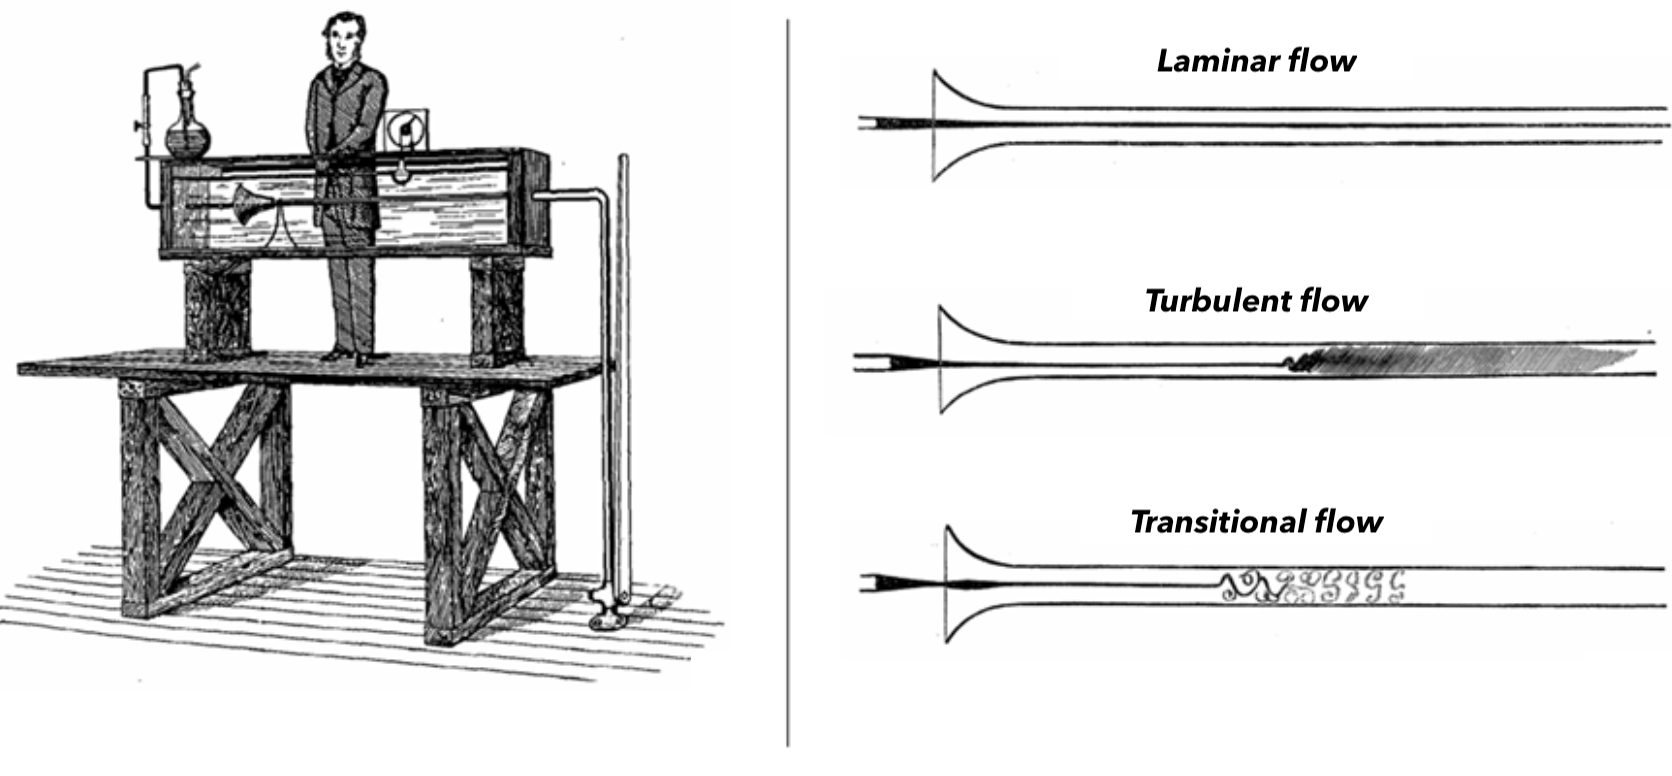
\includegraphics[width=1\textwidth]{grafici/reynolds_exp}
\caption{Sketch of the Reynolds experiment (\emph{left}) and flow patterns (\emph{right})}
\label{Reynolds:exp}
\end{center}
\end{figure}

with $u$ that is the characteristic velocity of the fluid, $l$ is the reference length of the scale and $\nu$ is the kinematic viscosity; able to predict the presence, or not, of the turbulence. He saw that when the inertia forces are huge the flow become unstable and the ink of its experiment started mixing with the surrounding water, as shown in the sketch of figure~\ref{Reynolds:exp}.
\par
This first work has correlated the presence of different states of the flow, laminar, transitional and turbulent, and their relationship with the couple viscous term-nonlinear inertia term.
Further observations revealed the presence of three-dimensional eddies. Although we are still unable to determine their shapes, we have understood that they play a key role in the turbulence sustenance. Under the assumptions of incompressible flow, not subjected to external forces of volume or surface, the vorticity equation states
\begin{equation}
\frac{D \boldsymbol{\omega}}{D t} = (\boldsymbol{\omega} \cdot \boldsymbol{\nabla})\boldsymbol{u} + \nu \boldsymbol{\nabla}^{2} \boldsymbol{u}.
\end{equation}
The central term of the equation, $ (\boldsymbol{\omega} \cdot \boldsymbol{\nabla})\boldsymbol{u}$, is known as vortex-stretching term. 
The vortex stretching is at the core of the description of the turbulent energy cascade, from the large scales to the smallest scale, determined, as we will see, by the turbulence itself.
For incompressible flow, due to volume conservation of fluid elements, the lengthening implies thinning of the fluid elements in the directions perpendicular to the stretching direction. This reduces the length scale of the associated vorticity. Finally, at the smallest scales the turbulence kinetic energy is dissipated into heat through the action of molecular viscosity~\cite{Lumley}.



\section{The history of the direct numerical simulation}
The direct numerical simulation (DNS) of the Navier-Stokes equations is a mathematical tool used to analyze turbulent flows since it allows to have an inner viewpoint in the transition and turbulence phenomena processes. It is part of the so called Computation Fluid Dynamics, or CFD, research field. 
Given the high computational cost of these simulations, DNS is not used to reproduce real-life flows, but as a research tool for flows with simple boundaries\cite{dns:tool}. \par
Despite of such kind of simulations, due to their limits, could seem useless, they assume relevant importance in the study of the turbulence, who, dominating the small scales, affect the behavior of the large scales, determining the raise of phenomenas such as flow separations, drag increases or losses of lift.
These simulations rely on high accuracy computational methods and they do not employ turbulence models, hence they require an ever-increasing computational power, as we move towards engineering relevant Reynolds numbers. 
However we can identify an ultimate threshold for direct numerical simulation of the wall bounded flows, which, thanks to its scale separation,  give the possibility to model the turbulence phenomena once for all. In~\cite{Jimenez2003} professor Jiménez set such threshold around $Re_{\tau}=10000$\\~\par




The DNS history is recent, with the first milestone work carried out by Kim, Moin and Moser~\cite{kim_moin_moser} in the 1987, using a $192\times 129 \times160$ grid of points distributed in a channel flow domain, in which they studied the homogenous isotropic turbulence using spectral modes. Follow this seminal work other authors proposed their simulations.
Accurate DNS calculations of the turbulent channel flow, using spectral methods, have been carried out by Lyons \emph{et al.}~\cite{Lyons}, Antonia \emph{et al.}~\cite{antonia_teitel_kim_browne_1992}, Kasagi \emph{et al.}~\cite{Kasagi}, Rutledge and Sleicher~\cite{Rutledge} in the first nineties. In the 1999 Moser \emph{et al.}~\cite{KMMans} proposed their $Re_{\tau}=590$ simulation, while to see the first channel flow simulation using finite differences we have to wait Abe \emph{et al.}~\cite{Abe} in 2001.\par
Other works, from the first years of the twenty-first century, are for example Iwamoto \emph{et al.}~\cite{Iwamoto} ones, Del Alamo and Jiménez~\cite{delalamo} and, the first simulation with $Re_{\tau}$ over a thousand, Del Alamo \emph{et al.}~\cite{delalamo2} work, in 2004. \par
Between 2004 and 2007 were presented different works, alternating the finite differences techniques with the more established spectral methods approach.
Tanahashi \emph{et al.}~\cite{Tanahashi}, Iwamoto \emph{et al.}~\cite{Iwamoto2}, Hoyas and Jiménez~\cite{Hoyas}, Hu \emph{et al.}~\cite{Hu}are some examples. \par
More recent simulation have been carried out by Lozano-Duràn \emph{et al.}~\cite{Lozano}, Lozano-Duràn and Jiménez~\cite{Lozano2}, Vreman and Kuerten~\cite{Vreman}, Bernardini \emph{et al.}~\cite{Bernardini} and the actually biggest simulation ever, with $Re_{\tau}=5200$, by Lee and Moser~\cite{Lee}. \par



The grows in $Re_{\tau}$ number is correlated with the grown in supercomputing performances on those years, as could be understood by looking at figures~\ref{top500} and~\ref{dns:trend}. However the $Re_{\tau}$ growth is not proportional with the computational power, as pointed out in~\cite{Jimenez2003}. In the same document is reported that a theoretical 500 Pflops supercomputer could carry out the $Re_{\tau}=10000$ simulation in a reasonable time. Unfortunately, starting from 2013, the rate of growth of the supercomputers speed has halved with respect to the past decade, and this made the forecast embedded in such document, false. With the current rate of growth it is more likely that we could carry out such simulation within the next three years. \\~\par



\begin{figure}
\begin{center}
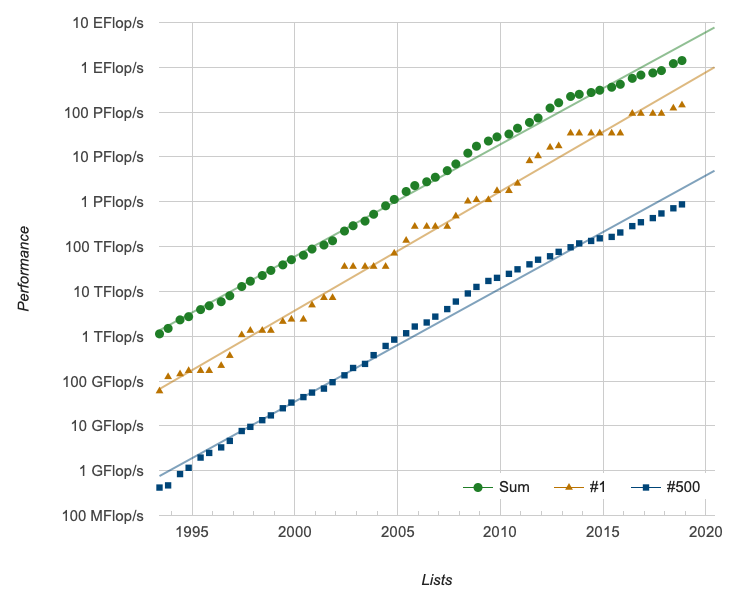
\includegraphics[width=0.8\textwidth]{grafici/top500hist}
\caption{Supercomputers grown trend, courtesy of TOP500.org}
\label{top500}
\end{center}
\end{figure}
\begin{figure}
\begin{center}
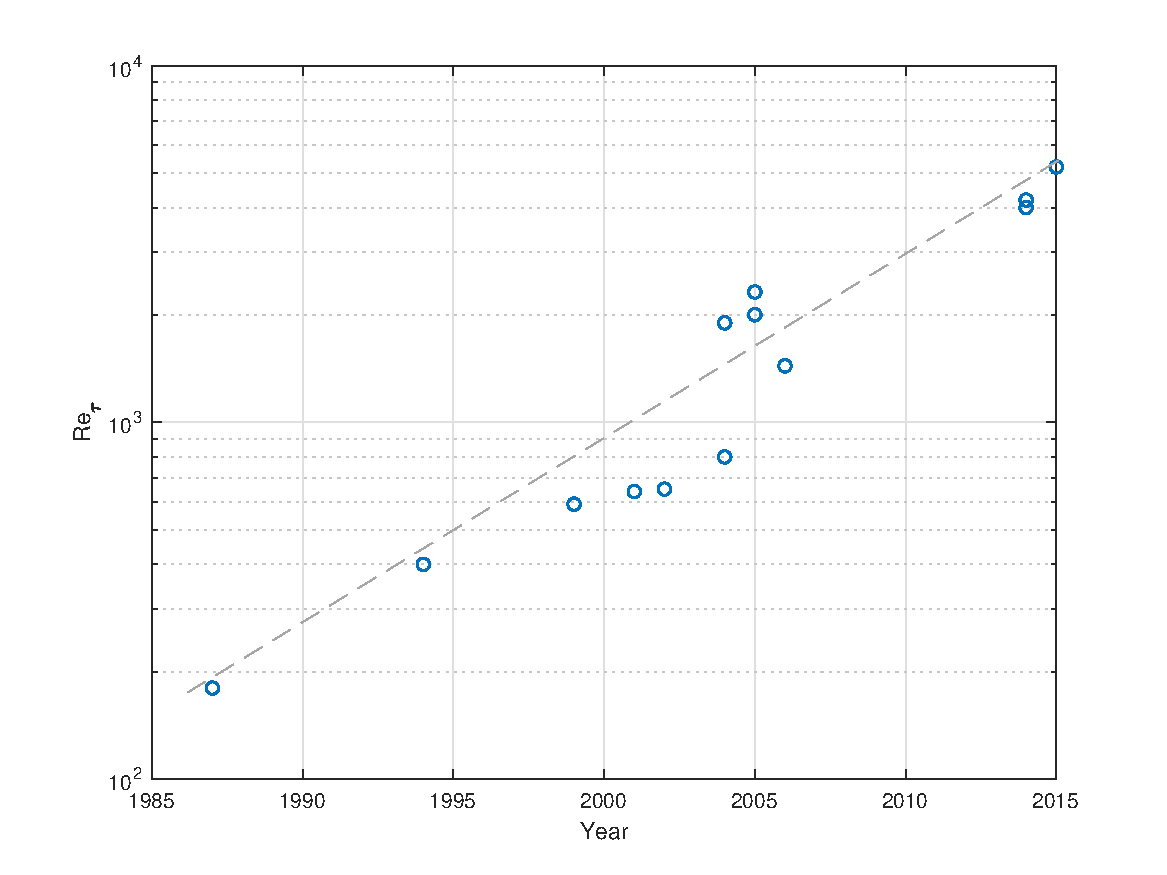
\includegraphics[width=0.8\textwidth]{grafici/dns_trend}
\caption{$Re_{\tau}$ grown trend}
\label{dns:trend}
\end{center}
\end{figure}



In this thesis our goal was to provide an highly parallelized DNS solver, based on pseudo-spectral approach, able to carry out simulation on a wide number of processors in the most efficient way possible. \par
We were particularly interested in the possibility to generate flow statistics at very high $Re_{\tau}$ values, in reasonable time, maintaining code efficiency above the 40\%. \\~\par

In this chapter we will provide a briefly description of the phenomena, then we will recall the main statistical quantities used to characterize turbulent flows. In the second chapter we will describe the geometry of the domain along with the governing equations for the problem presented, the structure of the code, discretization, domain decomposition and I/O.
The third chapter will deal with code benchmarks while the fourth will show the results of our simulations and the code validation against the well established $Re_{\tau}=180$ database of Kim, Moin and Moser. Finally we will draw a line of possible future works.






  




  
\chapter{Parallel DNS of a turbulent channel flow}


\section{Problem definition}
\pagestyle{headings}

Before moving to what has been done in this thesis I wish to briefly discuss the setup of our channel flow and the equations used to solve the problem.

\begin{figure}[h]
\centering
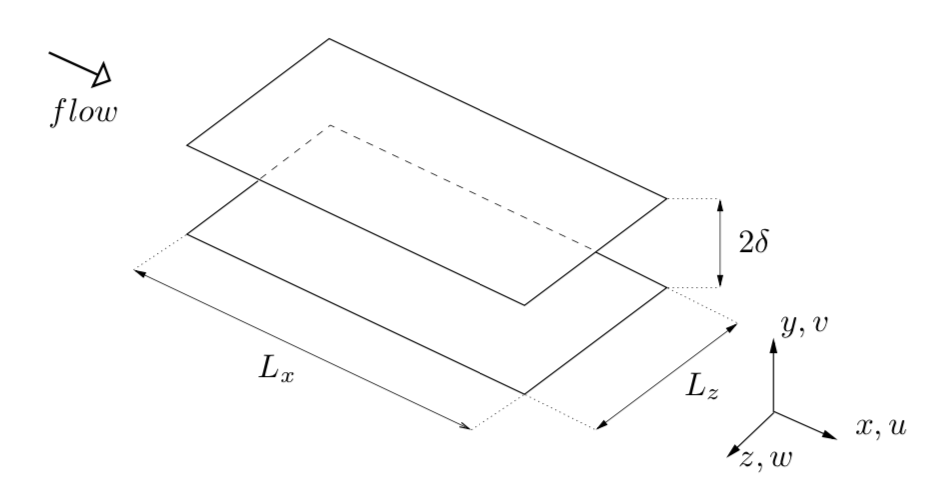
\includegraphics[width=0.8\textwidth]{grafici/sketch_dominio}
\caption{Domain of interest}
\label{sketch_dominio}
\end{figure}

We have the domain sketched in figure~\ref{sketch_dominio} where the $x$ and $z$ coordinates denote the streamwise and spanwise directions of the flow, while the $y$ coordinate is the wall normal ones.
Along these three dimensions we have $u,v$ and $w$ components of velocity.

The flow is assumed to be periodic in the streamwise and spanwise directions. The lower wall is at position $y_l$ and the upper wall at position $y_u$. The reference length $\delta$ is taken to be one half of the channel height.
Once an appropriate reference velocity is chosen, we can define the Reynolds number as:
\[
Re = \frac{U\delta}{\nu}
\]
where $\nu$ is the kinematic viscosity of the fluid.

According to our geometry and the assumption of incompressible flow, we can express the behavior of the flow through the mass conservation law:
\begin{equation}
\frac{\partial u}{\partial x} + \frac{\partial v}{\partial y} + \frac{\partial w}{\partial z} = 0
\label{mass:cons}
\end{equation}
 and the Navier-Stokes equations, which in a dimensionless form states:
\begin{subequations}
\label{eqn:ns}
\begin{align}
\frac{\partial u}{\partial t} + u\frac{\partial u}{\partial x} + v\frac{\partial u}{\partial y} + w\frac{\partial u}{\partial z} &= 
- \frac{\partial p}{\partial x} + \frac{1}{Re} \nabla^{2}u  \label{eqn:ns:1}\\
\frac{\partial v}{\partial t} + u\frac{\partial v}{\partial x} + v\frac{\partial v}{\partial y} + w\frac{\partial v}{\partial z} &= 
- \frac{\partial p}{\partial y} + \frac{1}{Re}\nabla^{2}v \label{eqn:ns:2}\\
\frac{\partial w}{\partial t} + u\frac{\partial w}{\partial x} + v\frac{\partial w}{\partial y} + w\frac{\partial w}{\partial z} &= 
- \frac{\partial p}{\partial z} + \frac{1}{Re}\nabla^{2}w \label{eqn:ns:3}
\end{align}
\end{subequations}
The differential problem is closed when initial conditions for all the fluid variables are specified, and suitable boundary conditions are chosen. At the walls the no-slip condition are imposed.








\section{Governing equations}
The numerical method does not rely on the equations~\eqref{eqn:ns}, instead it solves the wall-normal velocity and the wall-normal vorticity equations, recovering, at the end of the the solution, the three velocity components.\\
\subsection{Wall normal vorticity equation}
Defining the wall-normal component of the vorticity vector as:
\[
\eta = \frac{\partial u}{\partial z} - \frac{\partial w}{\partial x}
\]
which, in Fourier space, holds:
\[
\hat{\eta} = i\beta \hat{u} - i \alpha \hat{w}
\] 
with the hat indicating Fourier-transformed quantities, $i$ the imaginary part, $\alpha$ and $\beta$ the streamwise and spanwise wave numbers;  allows to write a one-dimensional second-order evolutive equation for $\hat{\eta}$ which does not involve pressure, as proposed in \cite{kim_moin_moser}.

Taking the y-component of the curl of the momentum equation we obtain:
\begin{equation}
\label{curl:momentum:y}
\frac{\partial \hat{\eta}}{\partial t}  = \frac{1}{Re}  \big( D_{2}(\hat{\eta}) - k^{2} \hat{\eta} \big) + i \beta \widehat{HU} -i \alpha \widehat{HW}
\end{equation}
where $D_{2}$ is the second derivative in the wall-normal direction, $k^{2}$ is the sum of $\alpha$ and $\beta$, and the nonlinear terms are defined as:

\begin{subequations}
\label{nonlinear:terms}
\begin{align}
\widehat{HU} &= i \alpha \widehat{uu} + D_{1} \widehat{uv} + i \beta \widehat{uw}\\ 
\widehat{HV} &= i \alpha \widehat{uv} + D_{1} \widehat{vv} + i \beta \widehat{vw}\\
\widehat{HW} &= i \alpha \widehat{uw} + D_{1} \widehat{vw} + i \beta \widehat{ww}.
\end{align}
\end{subequations}

To solve the equation \eqref{curl:momentum:y} we must set suitable initial conditions for $\hat{\eta}$. Such initial conditions are computed using the initial velocity field and the definition of $\eta$ itself.
Turning such conditions into frequency domain is straightforward and satisfy the periodic boundary conditions. Finally, the \emph{no-slip} condition for velocity vector enforce the condition at the walls, which, simply, translate in $\hat{\eta}=0$ at $y=y_{l}$ and $y=y_{u}$.


\subsection{Wall normal velocity equation}
An equation for the wall-normal velocity component $\hat{v}$, which does not involve pressure, is derived in \cite{kim_moin_moser}, by summing the equation \eqref{eqn:ns:1} derived two times w.r.t. $x$ and $y$, and \eqref{eqn:ns:3} derived two times w.r.t. $y$ and $z$, then subtracting \eqref{eqn:ns:2} derived w.r.t. $x$ and $x$ and substracting once again after derivation w.r.t. $z$ and $z$.
Further simplifications are invoked through the equation \eqref{mass:cons}, which lead to the following fourth-order evolutive equation for $\hat{v}$, which is the so called wall-normal velocity equation:
\begin{multline}
\label{normal:velocity}
\frac{\partial}{\partial t} \big( D_{2}(\hat{v}) - k^{2} \hat{v} \big) = \frac{1}{Re} \big( D_{4}(\hat{v}) - 2k^{2} D_{2}(\hat{v}) + k^{4} \hat{v} \big) \\
	-k^{2} \widehat{HV} - D_{1} \big(  i \alpha \widehat{HU} + i \beta \widehat{HW} \big).
\end{multline}
To solve such equation we have to enforce initial conditions on $\hat{v}$.\\
According to Fourier expansions, the periodic boundary conditions in the homogeneous directions are automatically satisfied, whereas the no-slip condition for the velocity vector immediately translates in $\hat{v} = 0$ to be imposed at the two walls.\\
The two remaining conditions for the fourth-order equation \eqref{normal:velocity} comes from the continuity equation \eqref{mass:cons}, written at the vertical edges of the domain, $y= y_{l}$ and $y=y_{u}$.


\subsection{Velocity components in the homogeneous directions and mean flow}
As reported before, once the two preceding equations are solved, we can use them to recover the velocity components in the homogeneous directions.\par
Assuming the non-linear terms \eqref{nonlinear:terms} known, as is the case when such terms are treated explicitly in the time discretization, the equations \eqref{curl:momentum:y} and \eqref{normal:velocity} become uncoupled and, after proper time discretization, can be solved for advancing the solution by one time step, provided the nonlinear terms \eqref{nonlinear:terms} and their spatial derivatives can be calculated.
To this aim, one needs to know how to compute $\hat{u}$ and $\hat{w}$ at a given time starting with the knowledge of $\hat{v}$ and $\hat{\eta}$. \\
By using the definition \eqref{curl:momentum:y} of $\hat{\eta}$ and the continuity equation \eqref{mass:cons} written in Fourier space, a 2 $\times$ 2 algebraic system can be written for the unknowns $\hat{u}$ and $\hat{w}$; its analytical solution read:

\begin{equation}
\begin{cases}
\label{uw:eq}
\hat{u} &= \dfrac{1}{k^{2}} ( i \alpha D_{1}(\hat{v} ) - i \beta \hat{\eta})\\\\
\hat{w} &= \dfrac{1}{k^{2}} (i \alpha \hat{\eta} + i \beta D_{1}(\hat{v}))
\end{cases}
\end{equation}
For $k^{2}=0$ the system of equation \eqref{uw:eq} is singular. \par
The present method therefore enjoys its highest computational efficiency only when Fourier discretization is used in the homogeneous directions.
\par
Since the previous system of equations \eqref{uw:eq} has been obtained starting from equations \eqref{curl:momentum:y} and \eqref{normal:velocity} the solutions are sensible to homogeneous spatial derivatives through the wave numbers. \par
Let us introduce a plane-average operator defined as:
\begin{equation}
\tilde{f} = \frac{1}{L_{x}} \frac{1}{L_{z}} \int_{0}^{L_{x}} \int_{0}^{L_{z}} f \,dx \,dz.
\end{equation}
If we apply such operator to our velocity components vector $\mathbf{V}$, it turns out that $\mathbf{V}(x,y,z,t)~=~\mathbf{\widetilde{V}}(y,t) $. According to this, our velocity components are function of time and wall-normal coordinate only. In Fourier domain this behavior is denoted by the absence of the wave numbers, so for $k^{2}=0$. \par

In agreement with our reference system, where the $x$ axis is aligned with the mean flow, the temporal average of $\tilde{u}$ will denote the mean velocity profile, whereas the temporal average of $\tilde{w}=0$ throughout the channel. \\
Anyway $\tilde{w}$ can be different from zero at different time and distance from the wall. \par

Finally, applying the plane-average operator to the components of the momentum equation let us compute the $\tilde{u}$ and $\tilde{w}$:
\begin{subequations}
\begin{align}
\frac{\partial{ \tilde{u}}}{\partial t} &=  \frac{1}{Re} D_{2} ( \tilde{u}) - D_{1}( \widetilde{uv}) + f_{x} \\
\frac{\partial{ \tilde{w}}}{\partial t} &= \frac{1}{Re} D_{2}( \tilde{w}) - D_{1} ( \widetilde{vw}) + f_{z}
\end{align}
\end{subequations}

 In these expressions, $f_{x}$ and $f_{z}$ are the forcing terms needed to force the flow through the channel against the viscous resistence of the fluid. For the streamwise direction, $f_{x}$ can be an imposed mean pressure gradient, and in the simulation the flow rate through the channel will oscillate in time around its mean value. $f_{x}$ can also be a time-dependent spatially uniform pressure gradient, that has to be chosen in such a way that the flow rate remains constant in time. The same distinction applies to the spanwise forcing term $f_{z}$: in this case however the imposed mean pressure gradient or the imposed mean flow rate is zero, while the other quantity will be zero only after time average.\\
\par
\par
What has been shown in this chapter is intended just to be a brief discussion. Further informations are available in~\cite[1-3]{cpl:presentazione}.


\chapter{Code Structure}
\section{Spatial discretization along homogeneous directions}
Our solver is based on a Fourier approach. Among the advantages of such approach we face the possibility to expansion of the unknown functions in terms of truncated Fourier series in the homogeneous directions. For example the wall-normal component $v$ of the velocity vector is represented as:
\begin{equation}
v(x,y,z,t) = \sum_{h=-nx/2}^{+nx/2} \sum_{l=-nz/2}^{+nz/2} \hat{v}_{hl}(y,t) e^{i\alpha x}e^{i \beta z}
\end{equation}
where:
\begin{equation}
\alpha = \frac{2\pi h}{L_{x}} = \alpha_{0} h; \quad \beta= \frac{2 \pi l}{L_{z}} = \beta_{0}l
\end{equation}

$h$ and $l$ are integer indexes corresponding to the streamwise and spanwise direction respectively, and $\alpha_{0}$ and $\beta_{0}$ are the fundamental wavenumbers in these directions, defined in terms of the streamwise and spanwise lengths $L_{x} = {2\pi}/{\alpha_{0}} $ and $L_{z} = {2 \pi}/{\beta_{0}}$ of the computational domain. The computational parameters given by the streamwise and spanwise lenght of the computational domain, $L_{x}$ and $L_{z}$ , and the truncation of the series, $nx$ and $nz$, must be chosen so as to miminize computational errors. For further details regarding the proper choice of a value of $L_{x}$ see~\cite{QuadrioMaurizio2003Issi}.

The convolutions required to solve the equations~\ref{curl:momentum:y} and~\ref{normal:velocity} are computationally expensive if carried out in the frequency domain. The same evaluation can be performed efficiently by first transforming the three Fourier components of velocity back in physical space, multiplying them in all six possible pair combinations and eventually retransforming the results into the Fourier space. Fast Fourier Transform algorithms are used to move from Fourier to physical space and viceversa. The aliasing error is removed by expanding the number of modes by a factor of at least $3/2$ before the inverse Fourier transforms, to avoid the introduction of spurious energy from the high-frequency into the low-frequency modes during the calculation~\cite{ns:quadrio}.





\section{Finite difference scheme}
The discretization of the wall-normal derivatives $D_{1}$, $D_{2}$ and $D_{4}$, required for the numerical solution of the present problem, is performed through finite difference (FD) compact schemes~\cite{finite:difference:scheme} with fourth-order accuracy over a computational molecule composed by five arbitrarily spaced grid points. We indicate here with $d_{1}^{j} (i), i = -2, \dots , 2$ the five coefficients discretizing the exact operator $D_{1}$ over five adjacent grid points centered at $y_{j}$ :
\begin{equation}
D_{1} \big( f(y) \big) \vert_{y=y_{j}} = \sum_{i=-2}^{2} d_{1}^{j} (i) f(y_{j+i})
\end{equation}
The basic idea of compact schemes can be most easily understood by thinking of a standard FD formula in Fourier space as a polynomial interpolation of a trascendent function, with the degree of the polynomial corresponding to the formal order of accuracy of the FD formula. Compact schemes improve the interpolation by replacing the polynomial with a ratio of two polynomials, i.e. with a rational function. This obviously increases the number of available coefficients, and moreover gives control over the behavior at infinity (in frequency space) of the interpolant, whereas a polynomial necessarily diverges. This allows a compact FD formula to approximate a differential operator in a wider frequency range, thus achieving resolution properties similar to those of spectral schemes~\cite{finite:difference:scheme}.
Compact schemes are also known as implicit finite-differences schemes, because they typically require the inversion of a linear system for the actual calculation of a derivative~\cite{compact:difference}\cite{finite:difference:scheme}.
 Here we are able to use compact, fourth-order accurate schemes at the cost of explicit schemes, owing to the absence of the third-derivative operator from the equations of motion. Thanks to this property, it is possible to find rational function approximations for the required three FD operators, where the denominator of the function is always the same, as highlighted first in the original Gauss-Jackson-Noumerov compact formulation exploited in his seminal work by Thomas~\cite{Thomas:coeff}, concerning the numerical solution of the Orr-Sommerfeld equations.\par
To illustrate Thomas’ method, let us consider an 4th-order one-dimensional ordinary differential equation, linear for simplicity, in the form:
\begin{equation}
D_{4}(a_{4}f) + D_{2}(a_{2}f)+D_{1}(a_{1}f)+a_{0}f = g,
\label{Thomas:coeff}
\end{equation}
Where the coefficients $a_{i}= a_{i}(y)$ are arbitrary functions of the independent variable $y$, and $g = g(y)$ is a known RHS. Let us moreover suppose that a differential operator, for example $D_{4}$, is approximated in frequency space as the ratio of two polynomials, say $\mathcal{D}_{4}$ and $\mathcal{D}_{0}$. Polynomials like $\mathcal{D}_{4}$ and $\mathcal{D}_{0}$ have their counterpart in physical space, and ${d}_{4}$ and $d_{0}$ are the corresponding FD operators. The key point is to impose that all the differential operators appearing in the example equation~\ref{Thomas:coeff} admit a representation such as the preceding one, in which the polynomial $\mathcal{D}_{0}$ at the denominator remains the same.\par
Equation~\ref{Thomas:coeff} can thus be recast in the new, discretized form:
\begin{equation}
d_{4} (a_{4}f) + d_{2} (a_{3}f) + d_{1} (a_{1}f) + d_{0} (a_{0}f) = d_{0} g,
\end{equation}
and this allows us to use explicit FD formulas, provided the operator $d_{0}$ is applied to the right-hand-side of our equations. The overhead related to the use of implicit finite difference schemes disappears, while the advantage of using high-accuracy compact schemes is retained~\cite{ns:quadrio}.





\subsection{Compute of the finite difference coefficients}










\section{Time Discretization}





\section{Domain Decompositions}
The engine of Quadrio and Luchini described into~\cite{cpl:presentazione} works per \emph{y-slabs}, as shown in figure~\ref{domain_decomp},
\begin{figure}
\centering
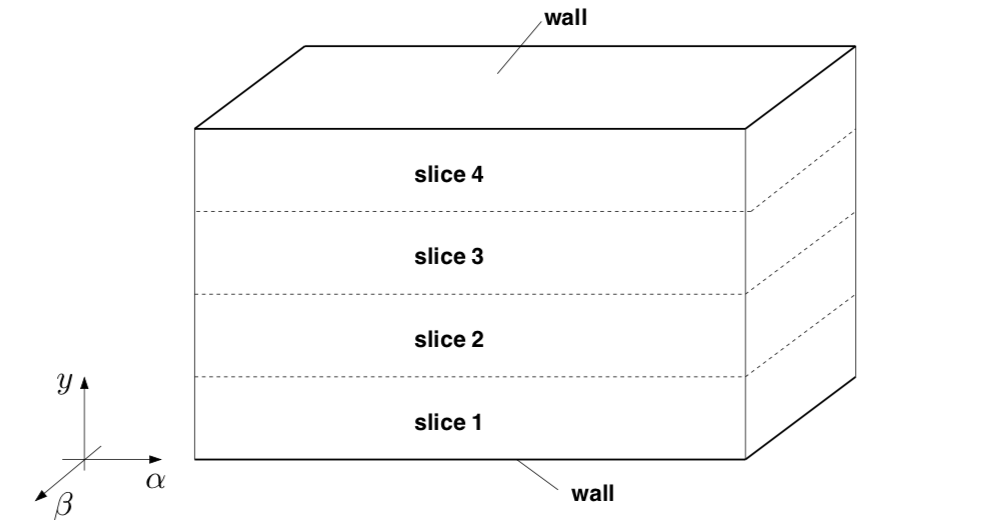
\includegraphics[width=0.8\textwidth]{grafici/decomp_dominio_cpl}
\caption{Original domain decomposition in case of 4 processors}
\label{domain_decomp}
\end{figure}
 allowing to perform convolutions and Fourier transformations locally on each processor, avoiding the cost of non-local transposition for the velocity array and the non-linear terms ones. Such implementation, denominated pipelined-linear-system (PLS), lead to a minimum of communication, in fact this approach require to send and receive only the values stored in the two upper and lower boundary cells of the local decomposition, in order to provide the data required by the fourth-order finite difference scheme.
 \par
 Using the PLS approach the number of bytes exchanged in a three step Range-Kutta method are:
 \begin{equation}
 D_{t} = 3 \times 8 \times (p-1) \frac{3}{2} \times \frac{nx}{p} \frac{nz}{p} \times ny \times 18
 \label{exchange:data:cpl}
 \end{equation}
 where:
 \begin{description}
  \item[3] takes into account the number of time steps;
  \item[8] for counting the bytes;
  \item[$\mathbf{(p-1)}$] is the number of nodes across which the exchange take place;
  \item[ $\mathbf{\frac{3}{2}}$ ] corresponds to the expansion in horizontal modes required by the dealiasing process;
  \item[ $\mathbf{\frac{nx}{p} \times \frac{nz}{p}}$] is the grid portion, for each plane, to exchange with the others nodes;
  \item[18] due to the 3 velocities plus the 6 products to be exchanged twice, before and after the FFT;
  \item[ny] takes into account the number of planes to be exchanged.
\end{description}
Further details about the PLS communications are available in \cite[\nopp chapter 4.2]{ns:quadrio}. \\
 \par
Although efficient for small processors grid, the performances of this approach falls quickly whether the processors number becomes comparable with \emph{ny}.  Furthermore the code structure limit the number of parallel process to be just a fraction of the \emph{ny} extension.
\par
To avoid such limitations and increase the number of parallel processes we decided to move from PLS approach to something different.
We have identified two possible solutions:
\begin{description}
  \item employ \textbf{slab} decomposition along x or z axis;
  \item employ \textbf{pencil} decomposition.
\end{description}
Both implementation require extensive use of the MPI paradigm and, possibly, a library to handle such decompositions.
We opted to employ OpenMPI\cite{openmpi} for what concern the MPI paradigm, in particular we entrust to the well established OpenMPI version 3.1, release 3.1.3.
The ideas behind the choice of such library rely on the fact the OpenMPI is released behind BSD license\cite{bsd:license}, it is designed to group different MPI implementation, avoiding fragmentation and forking problem\cite{faq:openmpi} and, although less optimized on proprietary fabric such as Intel Omni-Path fabric\cite{intel:omnipath}\cite{intel:intelmpivsopenmpi}, is wider spread.


 while, for the decomposition, we entrusted in a new library, released by the 


\subsection{Slabs decomposition}


\subsection{Pencil decomposition}


%\section{Parallel I/O}

Input-output could be a serious bottleneck if we do not pay the right attention.
In particular, when dealing with supercomputers, two major problems arise:
\begin{itemize}
\item needing of parallel I/O,
\item avoid endianness problem related.
\end{itemize}
As first thing let us introduce I/O.\par
\begin{wrapfloat}{figure}{l}{0pt}
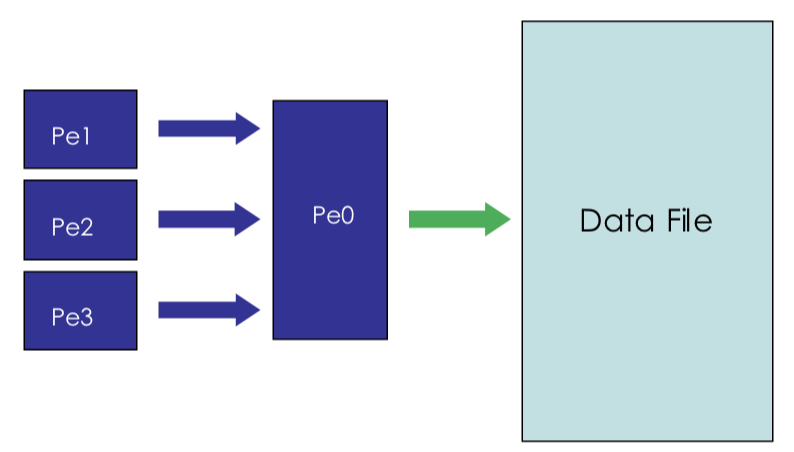
\includegraphics[width=0.5\textwidth]{grafici/masterslave}
\caption{Master-Slaves I/O setup}
\end{wrapfloat}
In computer architecture, the combination of the CPU and main memory, to which the CPU can read or write directly using individual instructions, is considered the brain of a computer. Any transfer of information to or from the CPU/memory combo, for example by reading data from a disk drive, is considered I/O~\cite{io}.
When dealing with cluster the transit of data from disk to CPU is not so straightforward. The presence of multiple CPU require the adoption of one of the following strategies.\par
The most basic strategy is the master-slaves setup. In this kind of strategy a single node of the grid have access to the storage, therefore no scalability is provided. The slave nodes must send/receive data from the master, therefore we face strong slowdown related to the huge workload required to perform I/O by the single node and the following communications among nodes.\par
A second approach is shown here beside and consist in performing distributed I/O on local files. Such kind of implementation is scalable, ensure data consistency and avoid communication during I/O phase. 
\begin{wrapfloat}{figure}{r}{0pt}
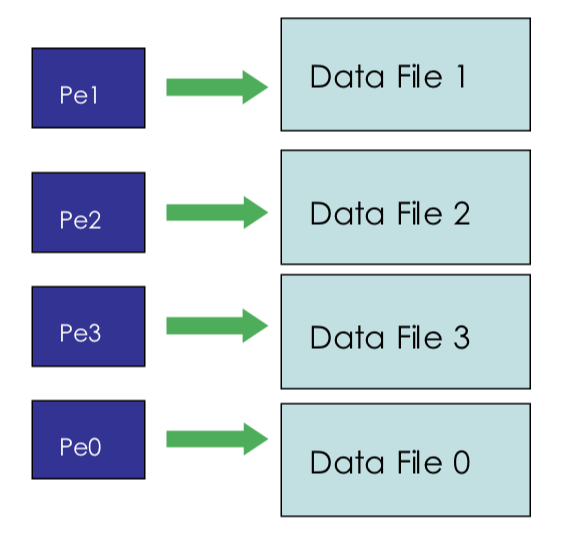
\includegraphics[width=0.5\textwidth]{grafici/localio}
\caption{Distributed I/O on local files}
\end{wrapfloat}However, since every processor writes data on its own hard storage, it require a great deal of post processing work to glue data among each others, which increase linearly with the number of processes. For this reason we can not consider it affordable. \\
\begin{wrapfloat}{figure}{r}{0pt}
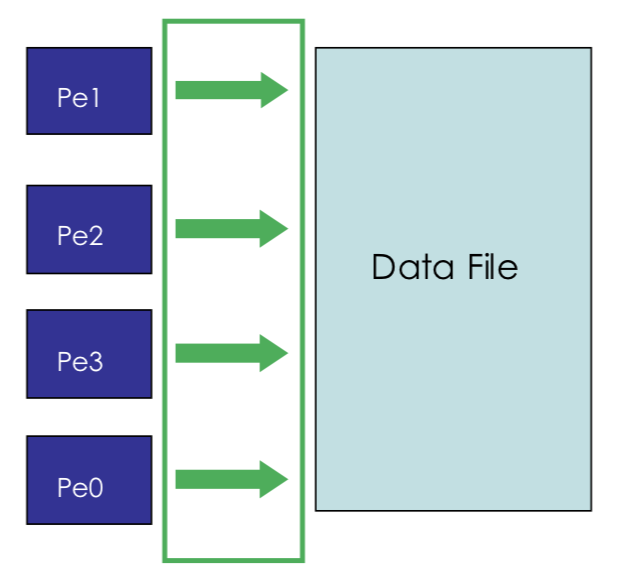
\includegraphics[width=0.5\textwidth]{grafici/mpiio}
\caption{Coordinated controlled accesses}
\end{wrapfloat}
\par
The last kind of I/O setup, which is the most updated and optimized, is the so called coordinated controlled accesses.
Scalability reaches its peak with this kind of implementation, which takes care of possible communications needing by its own.
In this approach every CPU can access to the single storage memory in which the dataset is hosted, and in concomitancy with the other processes, writes the data. As can be understood, the reading/writing operation is intrinsically fragile, since guarantee data consistency can be hard. To avoid consistency lacks, the MPI-IO has been introduced with the deployment of MPI-2 standard~\cite{MPI:standard2}.

On top of MPI-IO several high level I/O libraries arose, two well established examples are parallel netCDF and parallel HDF5. 

At exception of the master-slave approach, every presented strategy require the adoption of a parallel file system.
In computing, a file system or filesystem controls how data is stored and retrieved. Without a file system, information placed in a storage medium would be one large body of data with no way to tell where one piece of information stops and the next begins. By separating the data into pieces and giving each piece a name, the information is easily isolated and identified. We can briefly define the file system as the structure and logic rules used to manage the groups of information and their names.
In the same fashion a parallel file system maintains logical space and provides efficient access to data for distributed memory configurations.\\
\par
Let us establish the concept of endianness.
Intel introduces their white paper with the following sentence:\par
``Endianness describes how multi-byte data is represented by a computer system and is dictated by the CPU architecture of the system. Unfortunately not all computer systems are designed with the same Endian-architecture. The difference in Endian-architecture is an issue when software or data is shared between computer systems''\cite{endianness}.\par
Since our binary database has been built on Marconi, at Cineca, but the post-processing analysis take place on our personal computers, we need to guarantee results portability with a reliable method to store the data. \\
\par
Unfortunately MPI-IO can not set a bit ordering different from the machine's natives ones, and we can not assure portability in this way. To do so we have to move from MPI-IO to a library capable to satisfy our requirements.\par
Employ the well established parallel HDF5 library is the natural choice.





\chapter{Code Benchmarks}
The following chapter will show the performances obtained after the MPI integration in our code.
We have benchmarked three different problem sizes:
\begin{itemize}
\item small dimension problem $128\times 128 \times 128$;
\item medium dimension problem $512\times 512\times 512$;
\item large dimension problem $4096\times 512\times 512$.  
\end{itemize}
All problems have been tested using 1D and 2D decomposition, so that it is possible to have a comparison among this two methods.
\\
We want to highlight that all these problems exploit the Hermitian symmetry, along the streetwise axis.
\section{Testing environment}
Our test were conducted at CINECA\cite{Cineca}, an Italian academic research center, which host the $19^{th}$ most powerful supercomputers of the TOP500~\cite{top500} of November 2018 list.

We worked on Marconi\cite{marconi:specs} supercomputer, in particular on Marconi-A2 partition.
Marconi structure fuse different partition to reach the peak performance of 20 PFlop/s; in particular our partition is characterized by 3600 nodes, connected through Intel OmniPath\cite{intel:intelmpivsopenmpi} high performance network. Each node host a 68-cores Intel Xeon Phi 7250, code name Knight Landings, and about 100GB of ram. \\
The machine runs on CentOS 7.2~\cite{centos}, a Linux distribution, and our benchmark code has been compiled using GNU GCC 7.3~\cite{gcc} with OpenMPI 3.0.0~\cite{openmpi}\cite{MPI:standard3} . \\
\par
We have tested different flags during the compilation phase, trying to enable different levels of optimization and code vectorization, the most important feature of the Xeon Phi, however the best results have been achieved using:
\begin{lstlisting}
-O2 -fpic -march=native -std=c99
\end{lstlisting}
This behavior was expected since our code does not include the OpenMP\cite{openmp} features at present time, so the MIC\cite{mic} (Many Integrated Cores) architecture can not exploit such fundamental feature, possibly resulting in lack of performances and efficiency.



\section{Scaling performance of $128^3$ problem}
We proceed now showing the performances achieved by our code for the small problem.
This is likely the most critical benchmark for our code, since implement a distributed parallel approach to a problem with tiny dimensions could lead to lack of efficiency quickly. 
\par
In this kind of problem the arrays size fits the cache dimension of the Intel Xeon Phi processor; in fact, we achieve greater speedup by using less nodes as possible at cores equality. For this reason in this test we used 64 cores per node. 
\par
The results of figure \ref{641} shows that, although on single core the structure of the slab decomposed algorithm is faster, suddenly the benefits of pencil decomposition overcome the cost due to the poorer array storage.
To understand the latter sentence we should recall the figure of page \pageref{decomposition:example}.
Keeping in mind figure \ref{decomposition:example}, is possibile to understand why the slab decomposition is faster on single core, and typically also for a tiny cores number. Since the slab algorithm work \emph{per plan} we can, wisely, allocate and work just on a small dataset. This affect the communication phase, which will be faster if compared with the ones of the pencil decomposition that, instead, require to allocate all the data at once. 
\par

\begin{figure}
\begin{center}
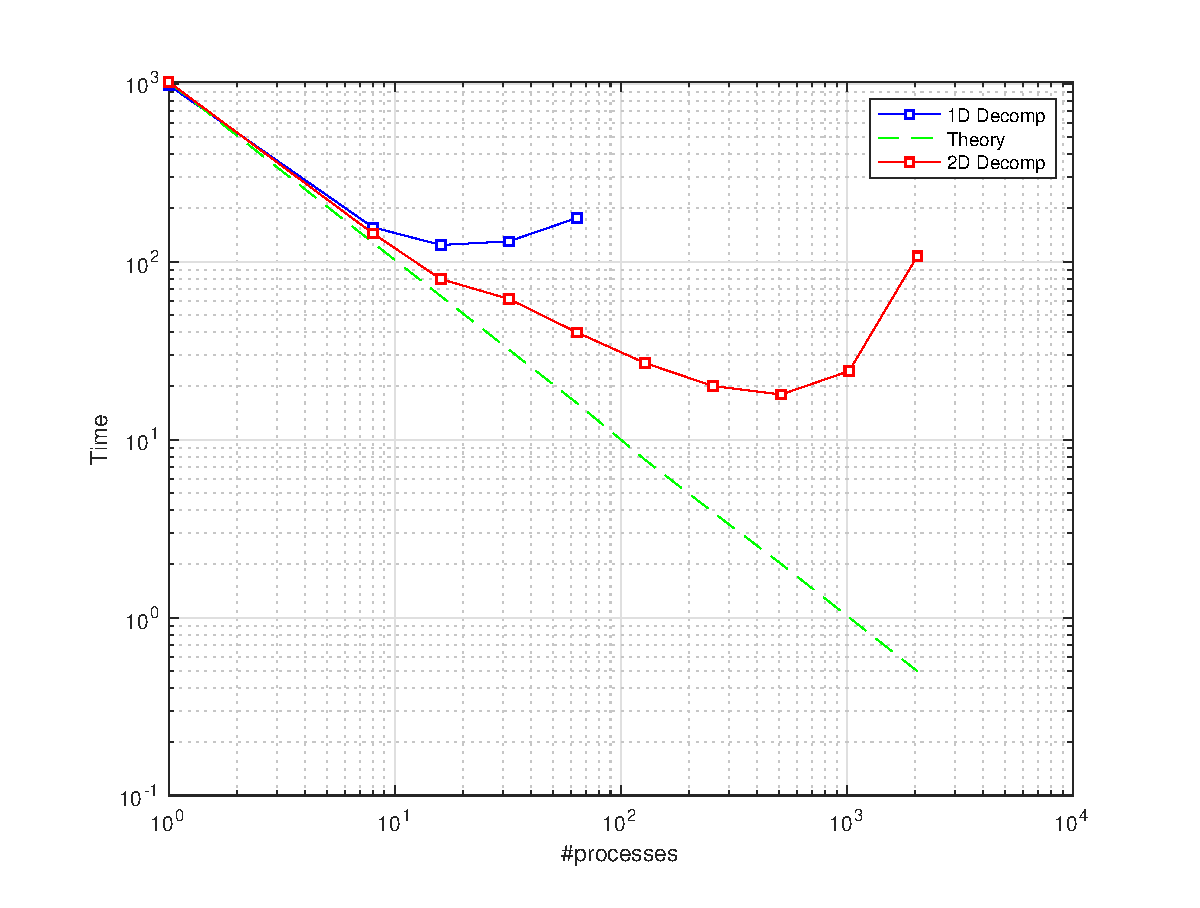
\includegraphics[scale=0.6]{grafici/641}
\caption{Scaling performance of $128^3$ simulation}
\label{641}
\end{center}
\end{figure}

In figure \ref{641} is possible to look at the time needed to perform the DNS, at varying of the cores number and algorithm.
The green dashed line represent the theoretical limit and has been obtained as the ratio between the single core time and the number of cores of the simulation.  \\
Despite of the results could seems poor, the qualitative comparison of figure~\ref{643} against a 3-dimensional FFT, using P3DFFT, reported in \cite[43]{tesi:brach}, suggest that our results are on the average, or better, until the communications cost overcome the benefits of such parallel distributed approach.

\begin{figure}
\begin{center}
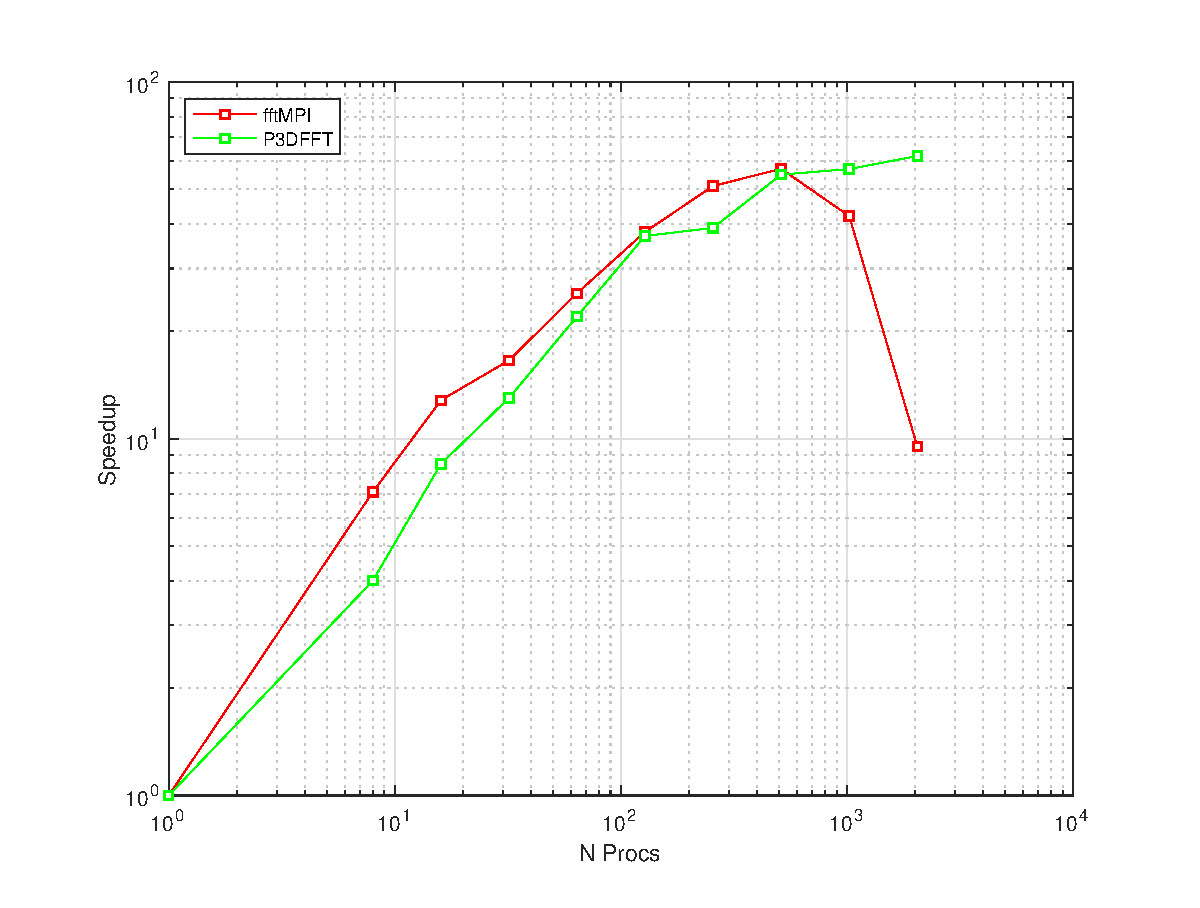
\includegraphics[scale=0.6]{grafici/643}
\caption{Comparison of a 3D FFT against DNS with fftMPI}
\label{643}
\end{center}
\end{figure}

\begin{table}[h]
\caption{Data from $128^{3}$ simulation}
\begin{center}
\begin{tabular}{c c c c}
\toprule
\textbf{\#cores} & \textbf{Time [s]} & \textbf{Speedup} & \textbf{Efficiency [\%]} \\
\midrule
\multirow{2}{*}{1} & 980 & 1.05 & 1.05 \\
& 1022.1 & 1 & 1 \\
\hline
\multirow{2}{*}{8} & 155.9 & 6.56 & 82 \\
& 144 & 7.1 & 89 \\
\hline
\multirow{2}{*}{16} & 124.2 & 8.24 & 52 \\
& 79.73 & 12.82 & 80 \\
\hline
\multirow{2}{*}{32} & 130.4 & 7.86 & 25 \\
& 61.65 & 16.6 & 52 \\
\hline
\multirow{2}{*}{64} & 176.1 & 5.81 & 9 \\
& 39.98 & 25.6 & 40 \\
\hline
128 & 26.9 & 38 & 30 \\

256 & 20 & 51.11 & 20 \\

512 & 17.91 & 57.07 & 11 \\

1024 & 24.28 & 42.1 & 4 \\

2048 & 107.3 & 9.52 & 0 \\
\bottomrule
\end{tabular}
\end{center}
\label{64data}
\end{table}%


The table~\ref{64data} on page~\pageref{64data} summarizes all data related to the $128^{3}$ simulation. 


\par
According to this table the figure \ref{642} shows the speedup at the varying of the cores number. \\
At the speedup peak the code runs $57$ times faster than serial ones. Such peak is obtained using $512$ cores. However, as expectable, the efficiency of this implementation is quite poor. In fact, if we use more than $16$ cores we drop immediately to performances around $50\%$ or lower. 
\par
Such speedup and efficiency have been calculated using the following definitions:
\[
S = \frac{T_{0}}{T_{p}} \quad \quad E = \frac{S}{p}
\]
where $T_{0}$ indicates the single core time, $p$ is the number of cores used in the actual run, and $T_{p}$ is the time associated with it. \\
\par
For completeness the efficiency behavior is reported in figure \ref{644}.

\begin{figure}
\begin{center}
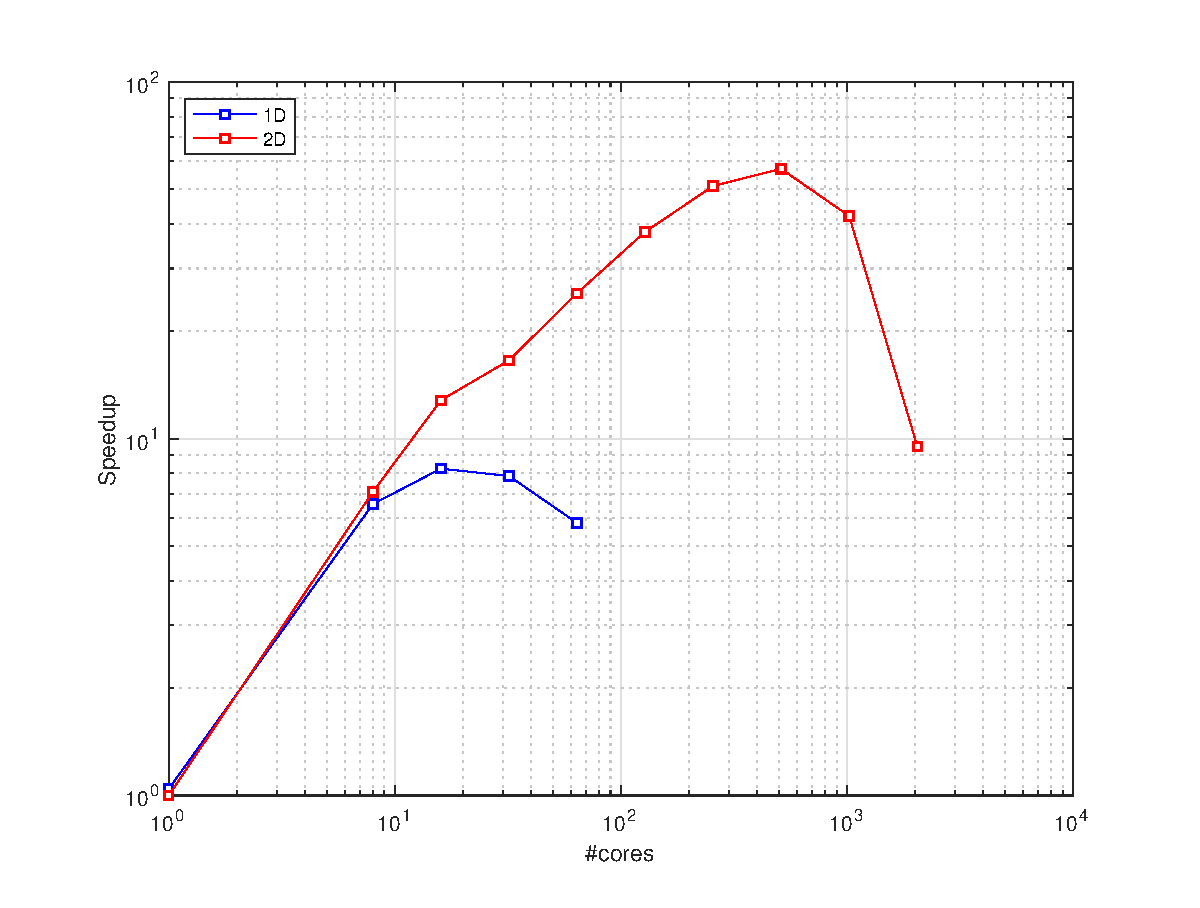
\includegraphics[scale=0.6]{grafici/642}
\caption{Speedup performance $128^3$ simulation}
\label{642}
\end{center}
\end{figure}

\begin{figure}
\begin{center}
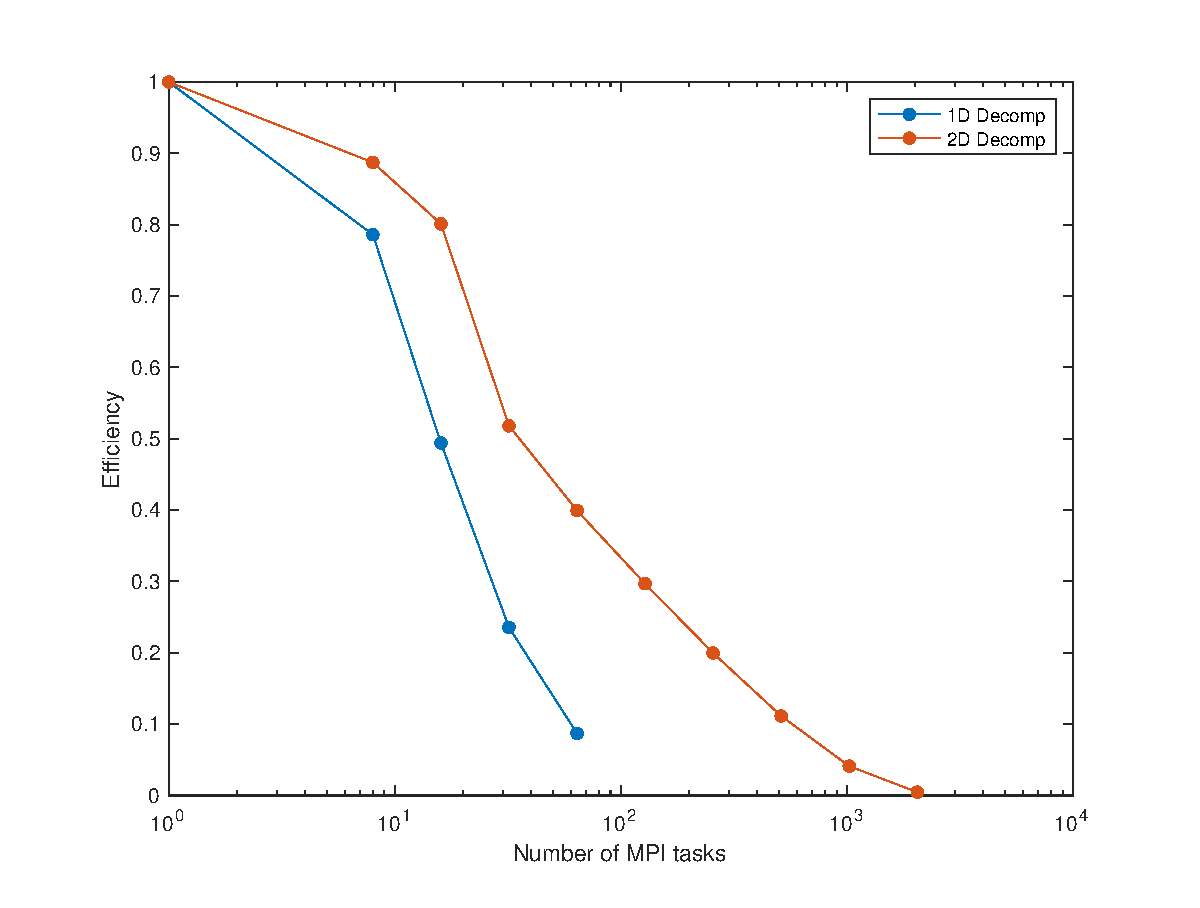
\includegraphics[scale=0.6]{grafici/644}
\caption{Efficiency behavior of $128^3$ simulation}
\label{644}
\end{center}
\end{figure}

\section{Scaling Performance of $256^{3}$ problem}
Many authors in past have highlighted how bigger problems provide better scaling capabilities and our $256^{3}$ simulation fulfill such trend.
The medium sized problem shows better scaling performances compared to the small ones, although exhibit a slightly rugged behavior.
\par
\begin{figure}
\begin{center}
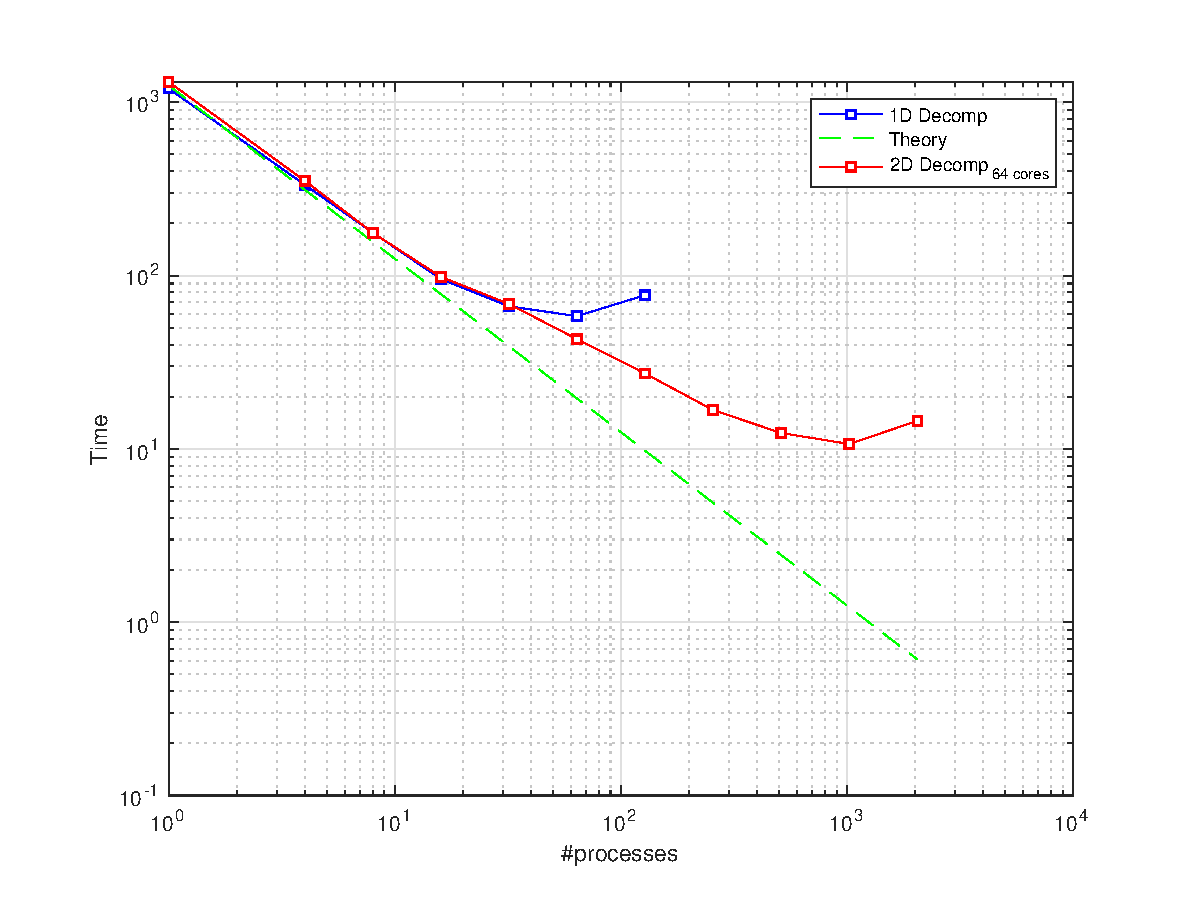
\includegraphics[scale=0.6]{grafici/1281}
\caption{Scaling performance of $256^{3}$ simulation}
\label{1281}
\end{center}
\end{figure}

\begin{figure}
\begin{center}
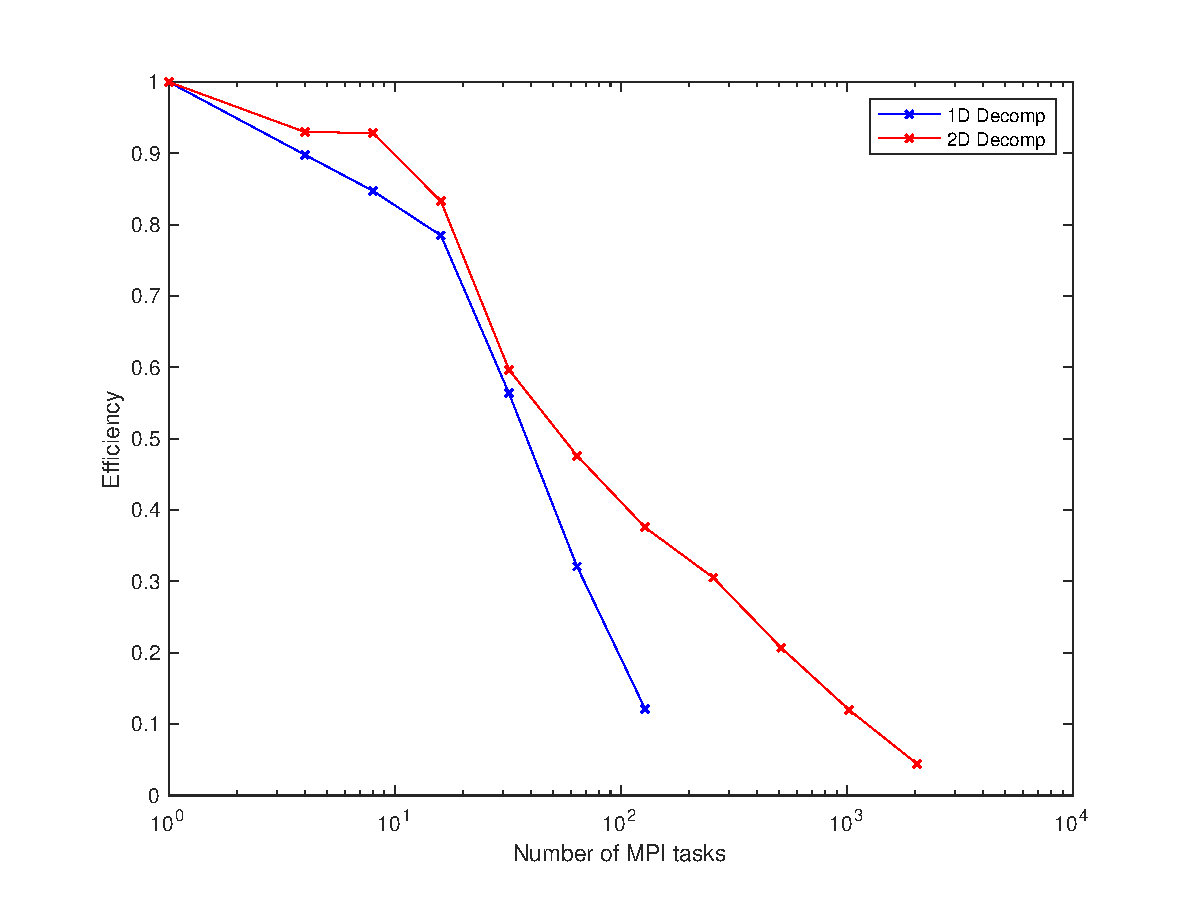
\includegraphics[scale=0.6]{grafici/1283}
\caption{Efficiency factor of $256^{3}$ simulation}
\label{1283}
\end{center}
\end{figure}

A slab decomposed algorithm provide gains of $\mathcal{O}(10)$ in terms of execution times, less than a pencil decomposed algorithm, but with better results for small processors grid. In fact, as depicted in figure~\ref{1281} the 1D decomposition curve achieve lower execution times than the 2D ones, until 32 cores.\\
Passed 32 cores the pencil decomposition prevails, reaching speedup factors above 120, with time savings in the order of magnitude of $\mathcal{O}(100)$ with respect to the single core runtime.
In the figure~\ref{1283} is possible to see the efficiencies achieved by the two methods, running on 64 threads per processor. It is important to denote the behavior of the pencil decomposed algorithm, which, until 8 cores are used, exhibits a very high scaling efficiency. \\
\par
Comparing image~\ref{1281} with its counterpart for the $128^{3}$ problem, figure~\ref{641} of page~\pageref{641}, we can see that the curves are quite similar. Both exhibits a very good fitting with the theoretical ones until 16 parallel processes take place. Once passed this threshold, the bigger problem maintains a better scaling efficiency, as we could see by comparing figure~\ref{1283} and~\ref{643}, for both decomposition methods. \par
The better efficiency allows to reach higher speedup factors at number of processes equality, and the larger dimensions move the performances peak towards higher number of threads, as is possible to see by looking at figure~\ref{1282}. The combination of this two factors doubles the last speedup factor, passing from 57, for the $128^{3}$ problem, to 122 for the $256^{3}$.\\

\begin{figure}
\begin{center}
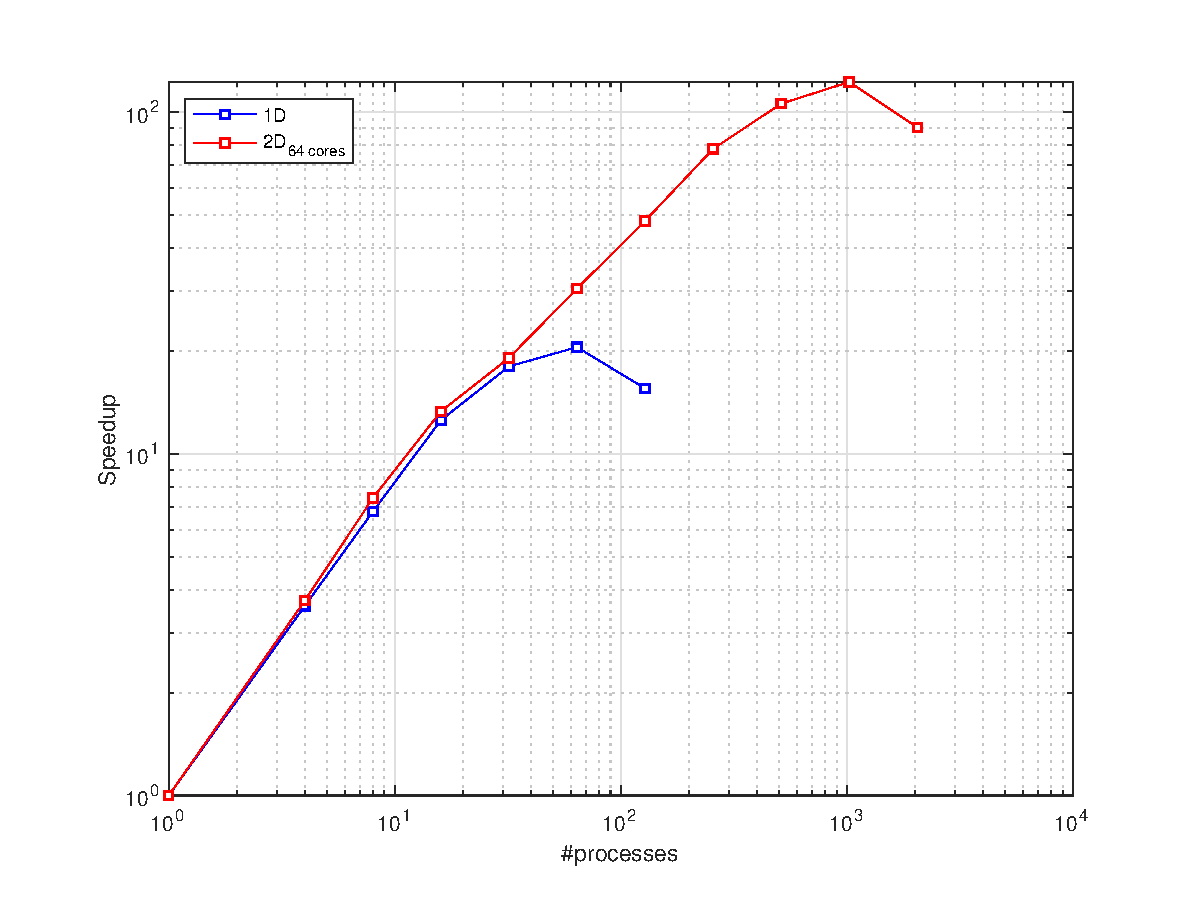
\includegraphics[scale=0.6]{grafici/1282}
\caption{Speedup performance factor of $256^{3}$ simulation}
\label{1282}
\end{center}
\end{figure}

\par
A comparison of the performances of 1D decomposition against the 2D for the present problem dimension is presented in table~\ref{128:data} of page~\pageref{128:data}.

\begin{table}
\caption{Data from $256^{3}$ simulation}
\begin{center}
\begin{tabular}{c c c c c}
\toprule
\textbf{\#Processes} & \textbf{Time [s]} & \textbf{Speedup} & \textbf{Efficiency [\%]} & \textbf{Decomp}\\
\midrule
\multirow{2}{*}{1} &  1198.8 & 1 & 100 & 1D\\
& 1309.7 & 14.28 & 89 & 2D\\
\hline
\multirow{2}{*}{4} &  333.7 & 3.59 & 90 & 1D\\
& 352.1 & 3.72 & 93 & 2D \\
\hline
\multirow{2}{*}{8} &  176.8 & 6.78 & 85 & 1D\\
& 176.3 & 7.43 & 93 & 2D\\
\hline
\multirow{2}{*}{16} & 95.5 & 12.56 & 78 & 1D\\
& 98.3 & 13.33 & 83 & 2D\\
\hline
\multirow{2}{*}{32} & 66.5 & 18.04 & 56.3 & 1D\\
& 68.6 & 19.1 & 60 & 2D\\
\hline
\multirow{2}{*}{64} & 58.4 & 20.54 & 32 & 1D\\
& 43 & 38.48 & 48 & 2D\\
\hline 
\multirow{2}{*}{128} & 77.1 & 15.55 & 12 & 1D\\
& 27.2 & 48.1 & 36 & 2D\\
\hline
256 & 16.8 & 78.19 & 31 & 2D\\
512 & 12.4 & 106.1 & 21 & 2D\\
1024 & 10.7 & 122.7 & 12 & 2D\\
2048 & 14.5 & 90.33 & 4 & 2D\\
\bottomrule
\end{tabular}
\end{center}
\label{128:data}
\end{table}


\par
Passed 8 cores, to recover high efficiency we must decrease the number of threads per processor. We have executed a detailed analysis varying the threads per processor number, seeking the optimization for both the decomposition methods.
\par
For what concern the slab decomposition the results, reported in table~\ref{128:data:1} on page~\pageref{128:data:1}, shows that, although slightly improvements have been achieved, the 1D decomposed algorithm is quite insensitive to cores per processor variations, showing constant speedups, efficiencies and timing.\\
\par 
\begin{figure}
\begin{center}
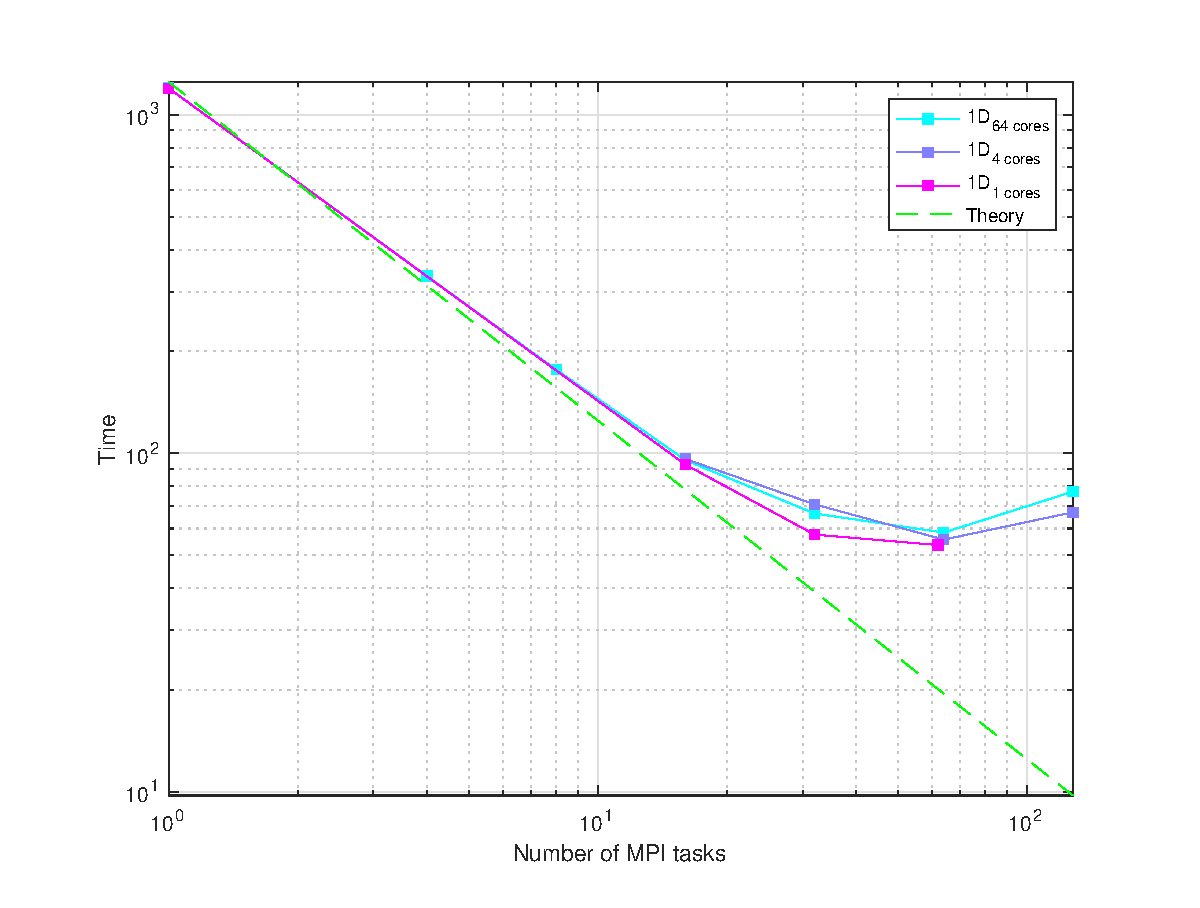
\includegraphics[scale=0.6]{grafici/1284}
\caption{Time scaling comparison using 1D decomposition for $256^{3}$ simulation}
\label{1284}
\end{center}
\end{figure}
\begin{figure}
\begin{center}
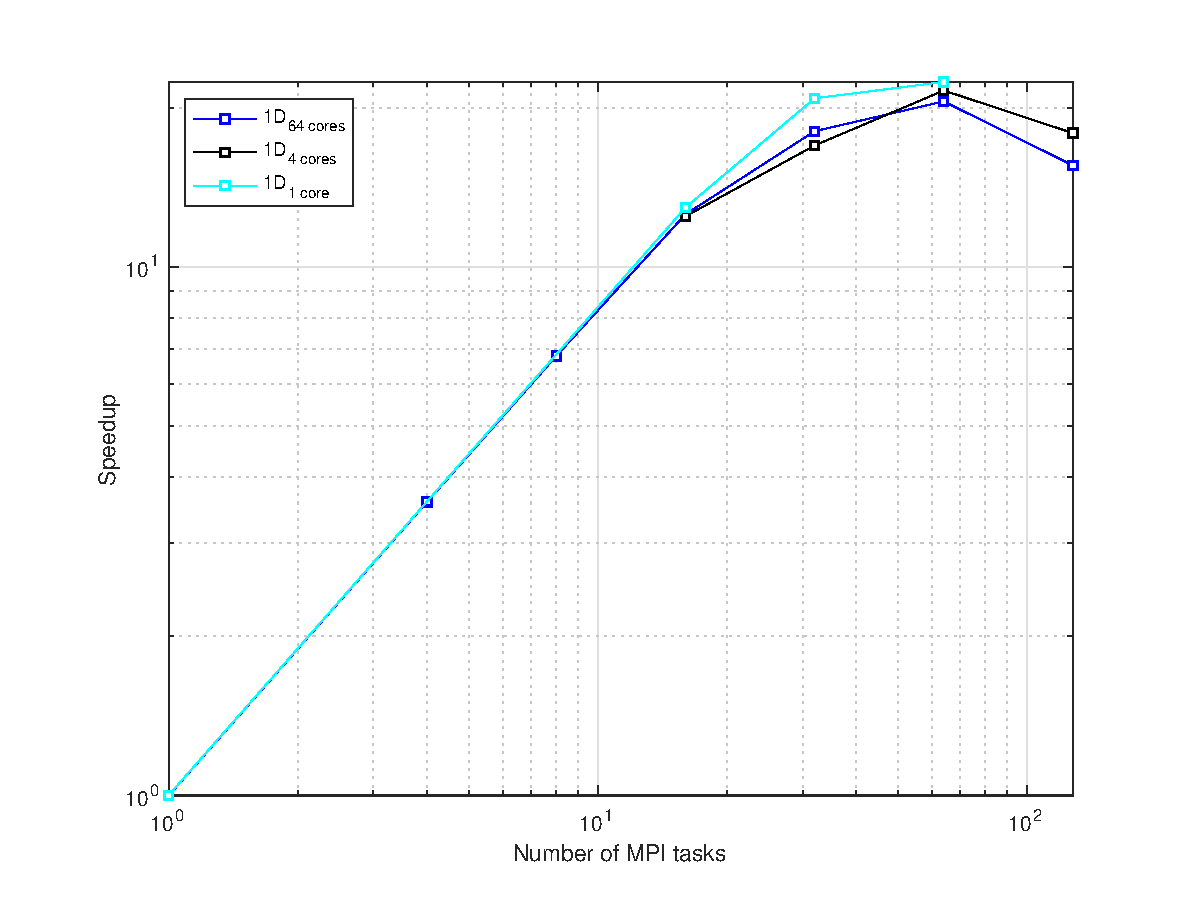
\includegraphics[scale=0.6]{grafici/1286}
\caption{Speedup comparison using 1D decomposition for $256^{3}$ simulation}
\label{1286}
\end{center}
\end{figure}
\begin{figure}
\begin{center}
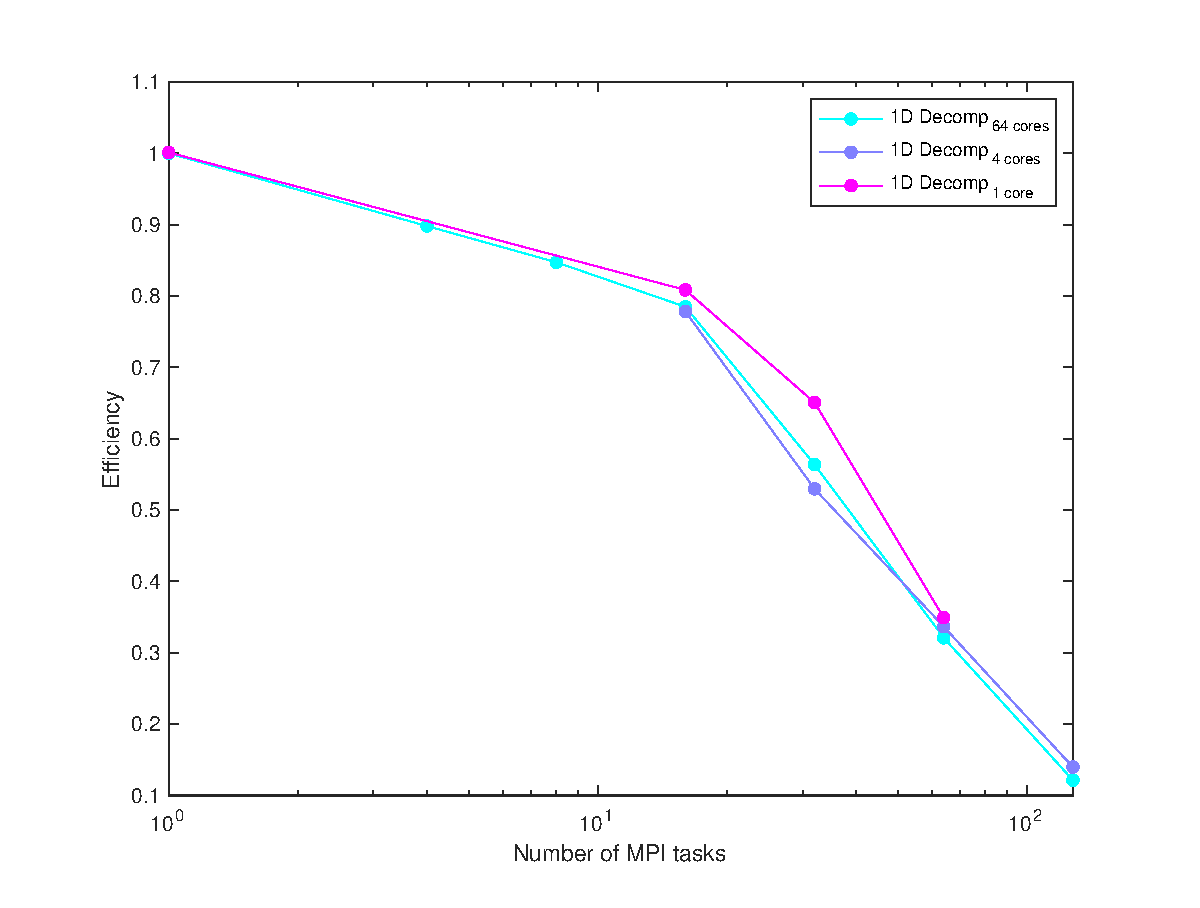
\includegraphics[scale=0.6]{grafici/1288}
\caption{Efficiency comparison using 1D decomposition for $256^{3}$ simulation}
\label{1288}
\end{center}
\end{figure}
Through figures~\ref{1284} and~\ref{1286} of page~\pageref{1284}, by looking at the single core curves, it is interesting to denote the presence of a knee, when 32 simultaneous processes take place, which origin a performances decrease. Such loss of linearity is present also using different cores per processor combinations, although on single core it appears to be more evident. Thus lead us to think that the intrinsic scaling limit, which depends on geometry and is caused by the raise in interprocessor communications time, has been reached. This limit clearly tear down the efficiency curve, as depicted in figure~\ref{1288}.\\

\begin{table}
\caption{Data from $256^{3}$ simulation, 1D decomposition}
\begin{center}
\begin{tabular}{c c c c c}
\toprule
\textbf{\#Processes} & \textbf{Time [s]} & \textbf{Speedup} & \textbf{Efficiency [\%]} & \textbf{cores}\\
\midrule
1 & 1198.75 & 1 & 100 & 64\\
4 &  333.7 & 3.59 & 90 & 64\\
8 &  176.8 & 6.78 & 85 & 64\\
\hline
\multirow{3}{*}{16} &  92.7 & 12.94 & 81 & 1\\
& 96.3 & 12.45 & 78 & 4\\
& 95.5 & 12.56 & 79 & 64\\
\hline
\multirow{3}{*}{32} &  57.6 & 20.82 & 65 & 1\\
& 70.7 & 16.95 & 53 & 4\\
& 66.5 & 18.04 & 56 & 64\\
\hline
\multirow{3}{*}{16} &  53.62 & 22.36 & 35 & 1\\
& 55.7 & 21.51 & 34 & 4\\
& 58.4 & 20.54 & 32 & 64\\
\bottomrule
\end{tabular}
\end{center}
\label{128:data:1}
\end{table}

\begin{table}
\caption{Data from $256^{3}$ simulation, 2D decomposition}
\begin{center}
\begin{tabular}{c c c c c}
\toprule
\textbf{\#Processes} & \textbf{Time [s]} & \textbf{Speedup} & \textbf{Efficiency [\%]} & \textbf{cores}\\
\midrule
1 & 1309.7 & 1 & 100 & 64 \\
4 & 352.1 & 3.72 & 93 & 64\\
8 & 176.3 & 7.43 & 93 & 64\\
16 & 98.3 & 13.33 & 83 & 64\\
\hline
\multirow{2}{*}{32} & 49.9 & 26.26 & 82 & 4\\
& 68.6 & 19.1 & 60 & 64\\
\hline
\multirow{2}{*}{64} & 29.3 & 44.73 & 70 & 4\\ 
 & 43 & 30.48 & 48 & 64\\
\hline
\multirow{4}{*}{128} & 21.4 & 61.17 &  48 & 4\\
& 21.5 & 61.03 & 48 & 8\\
& 23.2 & 56.58 & 44 & 32\\
& 27.2 & 48.1 & 38 & 64\\
\hline
\multirow{4}{*}{256} & 11.5 & 113.9 & 44 & 4\\
& 11.8 & 110.9 & 43 & 8\\
&13.5 & 97.23 & 38 & 32\\
&16.75 & 78.19 & 31 & 64\\
\hline
\multirow{4}{*}{512} & 9.4 & 140.1 & 27 & 4\\
&9.6 & 136.7 & 27 & 8\\
&11.8 & 110.7 & 22 & 32\\
&12.4 & 106.1 & 21 & 64\\
\hline
\multirow{3}{*}{1024} & 7.3 & 178.9 & 17 & 8\\
&9.9 & 132.7 & 13 & 32\\
&10.7 & 122.7 & 12 & 64\\
\hline
2048 & 14.5 & 90.33 & 4 & 64\\
\bottomrule
\end{tabular}
\end{center}
\label{128:data:2}
\end{table}

\par
Far more interesting is the pencil decomposed algorithm behavior. The data of such simulation, reported in table~\ref{128:data:2} of page~\pageref{128:data:2}, shows relevant improvements by varying the number of cores per processor. Another not yet cited, but always present tuning using 2D decomposition, is related to processor grid balancing. Our code provide optimal results when the processors grid have the same amount of MPI tasks among the two dimensions. Such behavior has been already described in deep in~\cite[39]{tesi:brach}. However it is not always possible to have the same number of threads in the two dimensions. In this case, after proper benchmark, we found that better results where achieved whether the number of tasks which decomposed the streamwise direction was lower than the other.
\par

\begin{figure}
\begin{center}
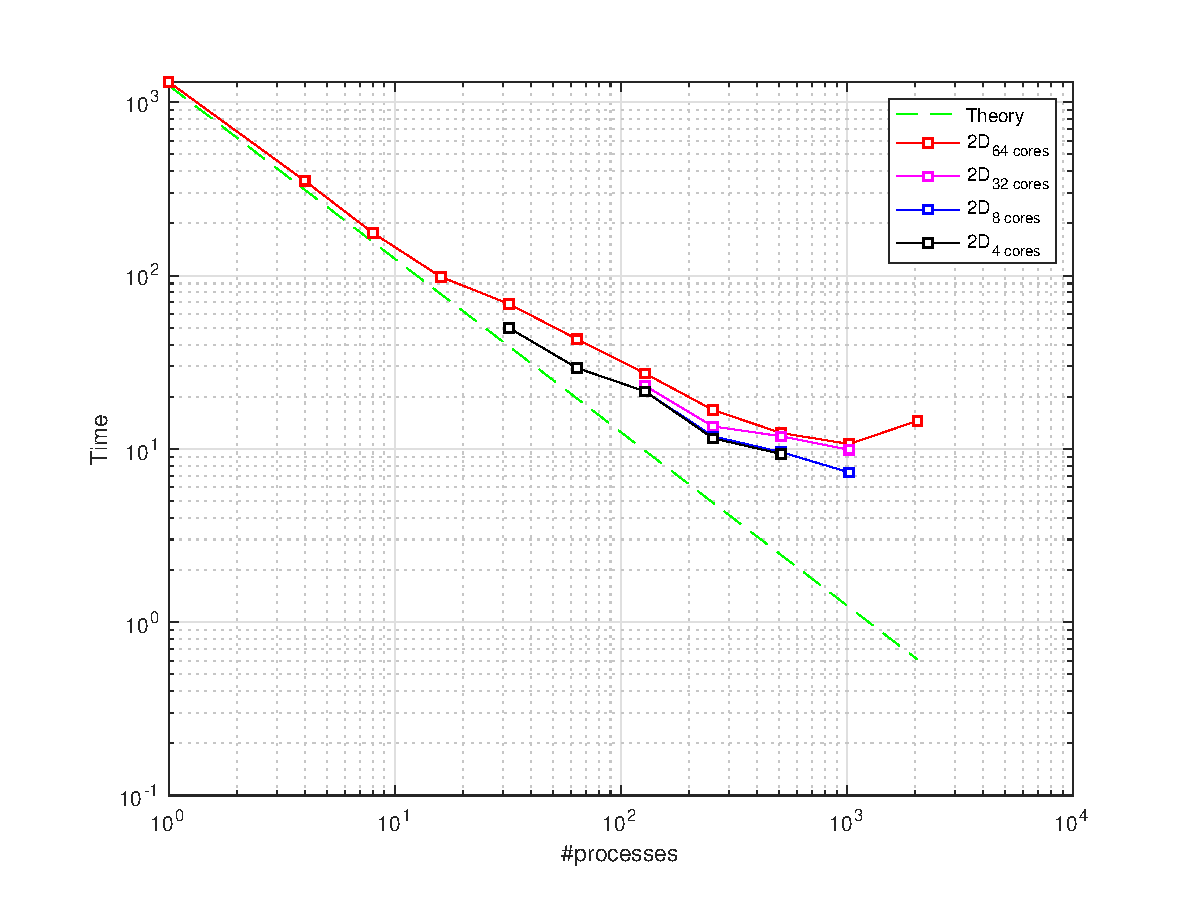
\includegraphics[scale=0.6]{grafici/1285}
\caption{Time scaling comparison using 2D decomposition for $256^{3}$ simulation}
\label{1285}
\end{center}
\end{figure}

As already said, the gains that we can obtain by reducing the number of threads per processor are high. 
Thus is due to the MPI standard that, although able to handle SMP processors~\cite{smp:processors}, lacks in efficiency as the number of cores becomes higher.
This is well highlighted by figure~\ref{1285}, in which we can see that a 4 cores approach can provide similar, or better, results than running the same code on 64 cores using twice the number of processes. The same reasoning holds also for an 8 versus 64 cores code execution. \par
This provide a boost in terms of execution time and, consequently, in terms of speedup factor, as can be recovered by looking at the results in table~\ref{128:data:2} where, at the peak, our speedup pass from 122.7 to 178.9.\par
The figure~\ref{1285} allow to see how, reducing the number of cores per processor, influence also the efficiency. Indeed we can see that running the code on 32 parallel processes using just 4 threads per nodes tends to realign the curve to the theoretical ones.\par
The efficiency curves can be seen in figure~\ref{1289}. They exhibit a rugged behavior with a marked trend to moves rightward as the number of cores per processor decreases.
For completeness the speedup factor curves has been reported, in figure~\ref{1287}.

\begin{figure}
\begin{center}
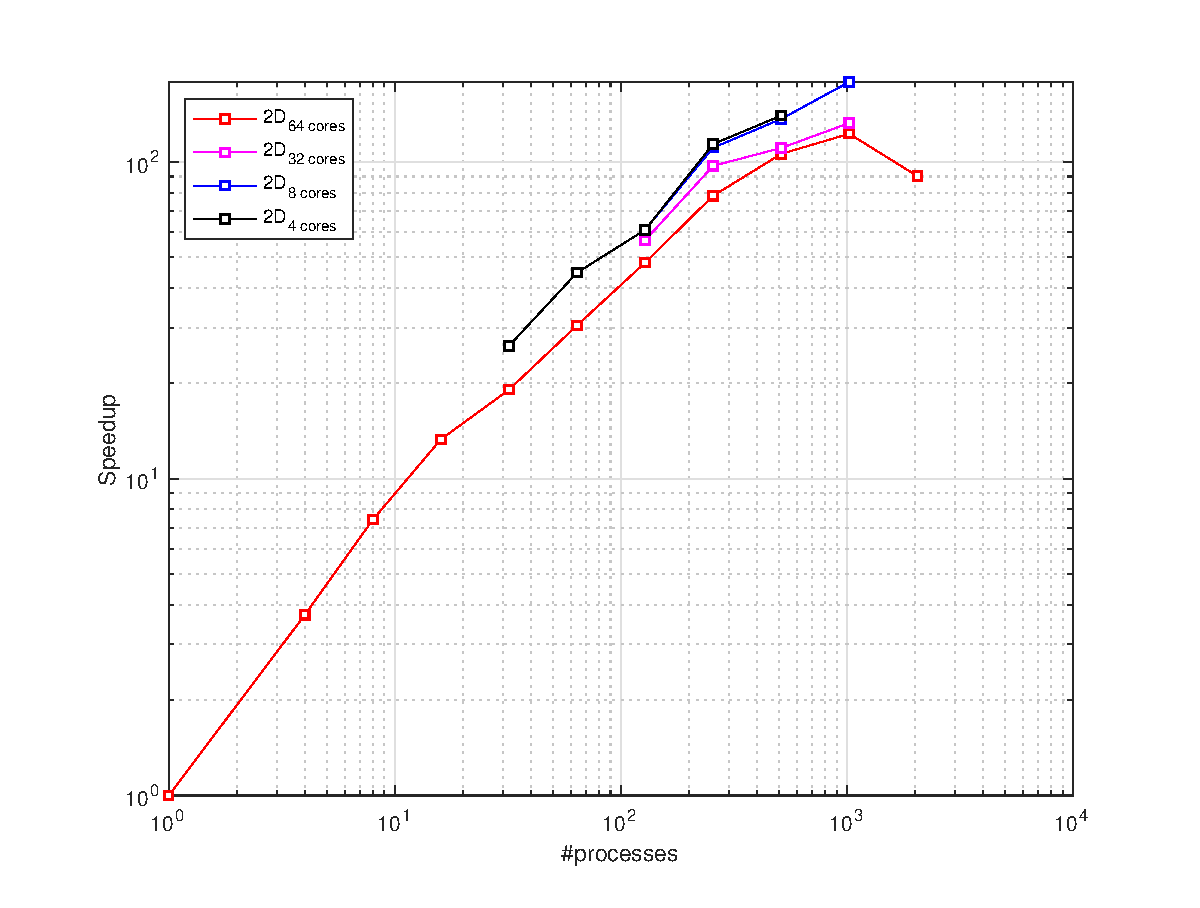
\includegraphics[scale=0.6]{grafici/1287}
\caption{Speedup comparison using 2D decomposition for $256^{3}$ simulation}
\label{1287}
\end{center}
\end{figure}

\begin{figure}
\begin{center}
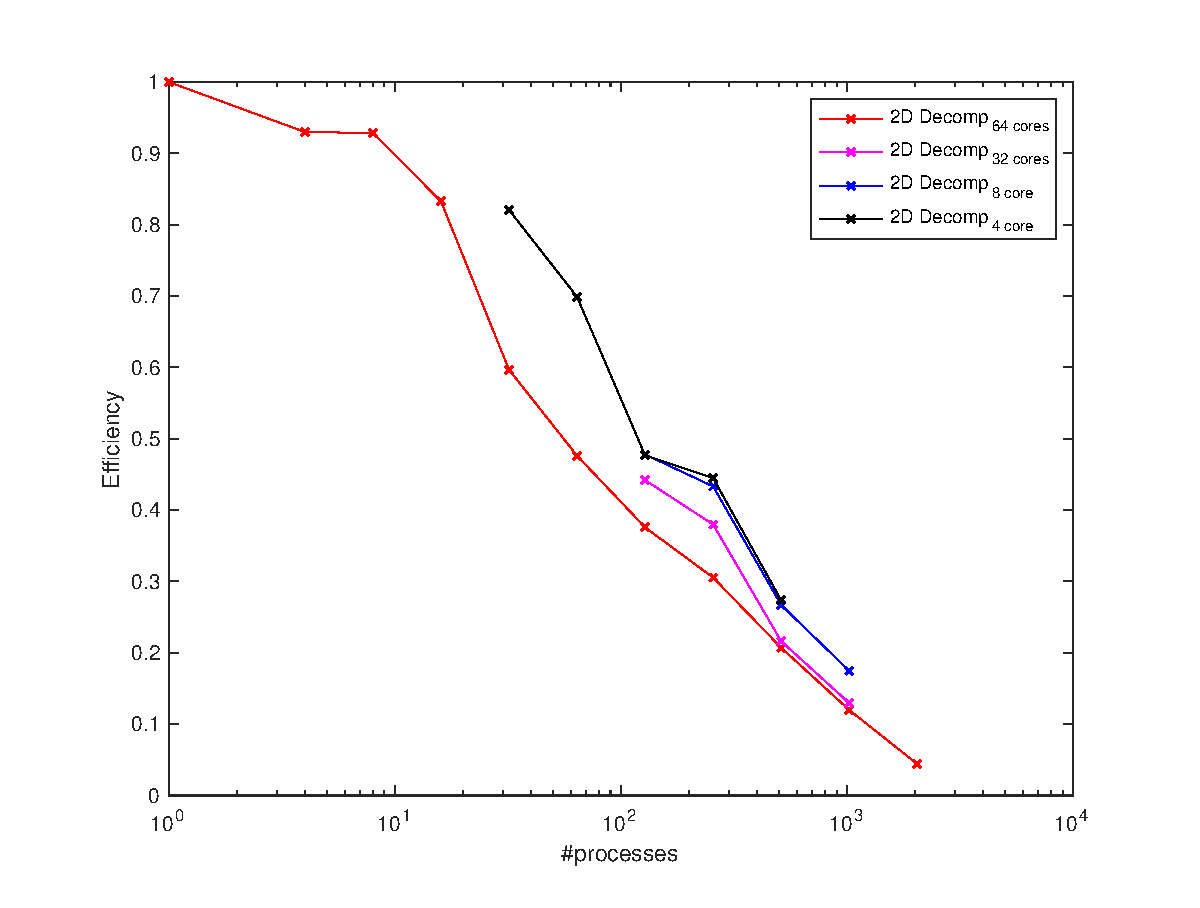
\includegraphics[scale=0.6]{grafici/1289}
\caption{Efficiency comparison using 2D decomposition for $256^{3}$ simulation}
\label{1289}
\end{center}
\end{figure}


\section{Scaling Performance of $512^3$ problem}
\pagestyle{headings}
\section{Scaling Performance of $4096\times512\times256$ problem}
The last benchmark deal with very large problems. Like for the previous large problem, the dimensions are so huge to require the adoption of multiple processors to run, otherwise we will face an out of memory error.
On a Intel Xeon Phi~\cite{intel:xeonphi} the minimum requirements are to employ at least 2 processors and use 32 cores, or less, per processor.
\par
As the previous problem have highlighted, the less cores are used and the better results are scored, so our impossibility to go further than 32 cores per processor, as pointed some rows before, would not be a big deal. We may suppose that the poorest results will be achieved by 32 cores runs, instead of the 64 ones. \\
\par

\begin{figure}
\begin{center}
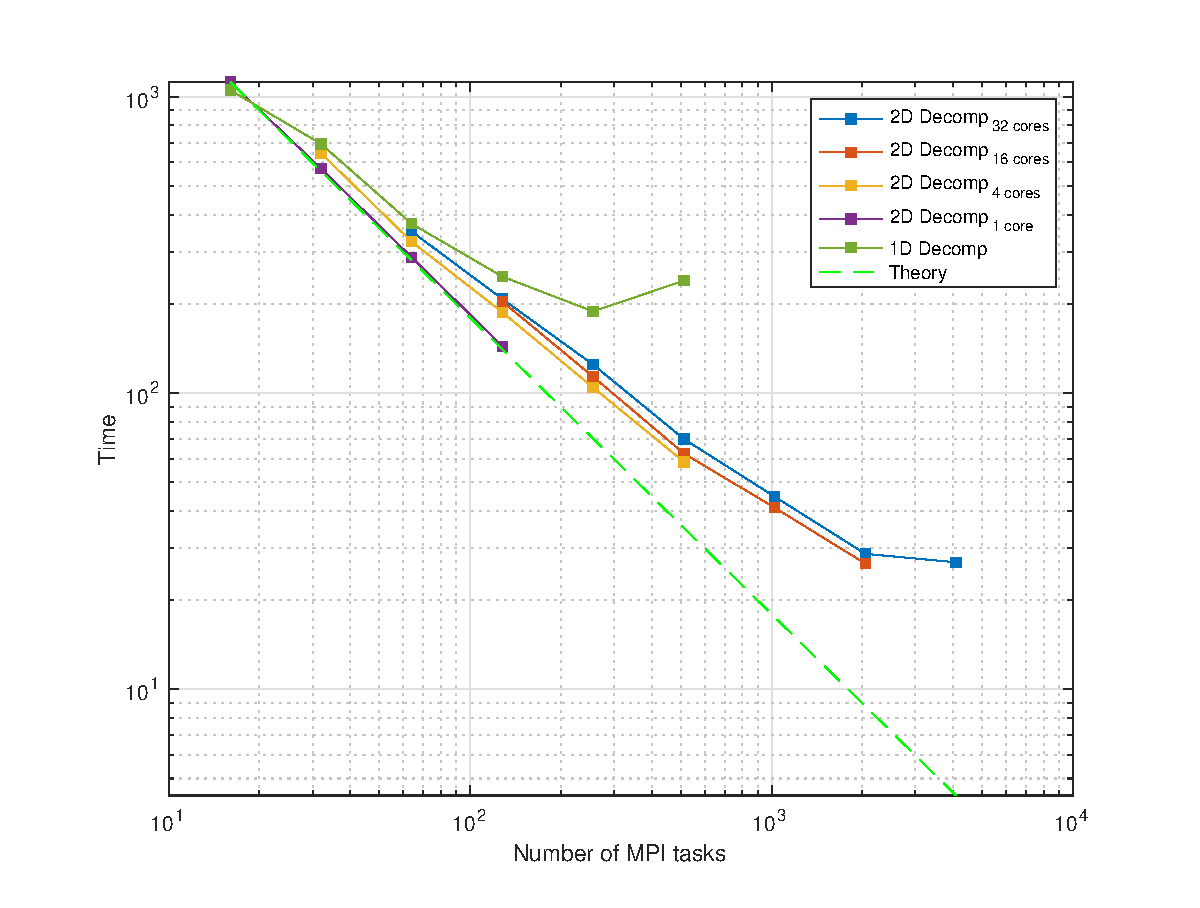
\includegraphics[scale=0.6]{grafici/20481}
\caption{Time scaling comparison for $4096\times 512\times 256$ simulation}
\label{20481}
\end{center} 
\end{figure}

Let us start showing figure~\ref{20481} in which is reported the time scaling of our code.\par
As could be seen, the 2D decomposition using single core achieved the lowest timing execution.
It is interesting to denote how this combination fits the theoretical behavior perfectly.\par
All other 2D decomposed combinations exploit a worse behavior with respect to the single core run, with a marked trend, where the increase in cores per processor number leads to poorer performances. \par 
Such behavior is aligned with our predictions.\\

\begin{figure}
\begin{center}
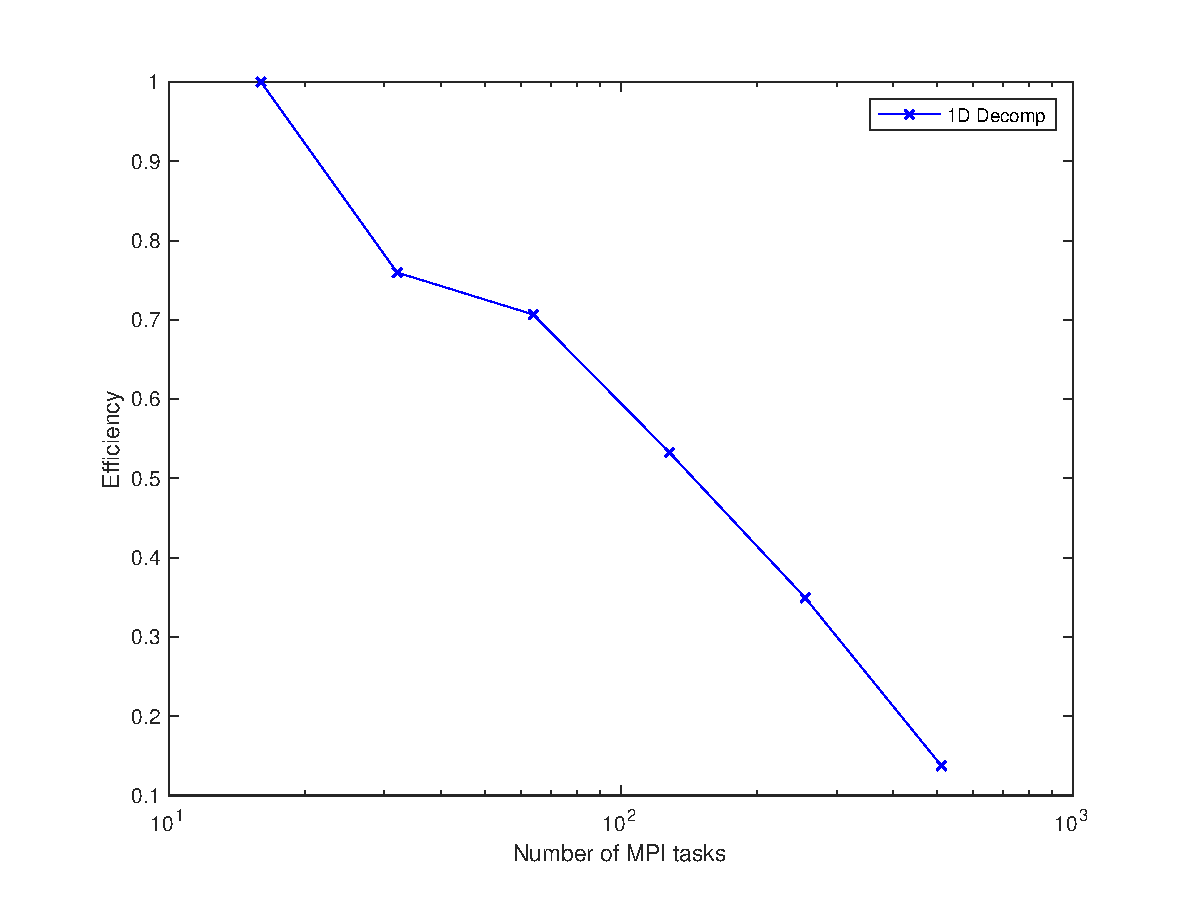
\includegraphics[scale=0.6]{grafici/20483}
\caption{Efficiency factor of $4096\times512 \times256$ simulation using 1D decomposition}
\label{20483}
\end{center}
\end{figure}

\begin{table}
\caption{Data from $4096\times 512\times 256$ simulation, 1D decomposition}
\begin{center}
\begin{tabular}{c c c c}
\toprule
\textbf{\#Processes} & \textbf{Time [s]} & \textbf{Speedup} & \textbf{Efficiency [\%]}\\
\midrule
16 & 1052.9 & 16 & 100\\
32 & 693 & 24.31 & 76\\
64 & 372.5 & 45.23 & 71\\
128 & 247 & 68.2 & 53\\
256 & 188.5 & 89.37 & 35\\
512 & 239.5 & 70.34 & 14\\
\bottomrule
\end{tabular}
\end{center}
\label{2048:data:1}
\end{table}

\par
For what concern about the 1D decomposed algorithm, which, since the code structure is slightly different, can run also on 64 cores per processor, it achieve the worst performances among all possible solutions, highlighting once again the benefits of using a pencil decomposed approach. \par
The speedups achieved by this kind of domain decomposition can be seen in table~\ref{2048:data:1}, on page~\pageref{2048:data:1}, while the efficiency graph, which shows a poor behavior, can be seen in figure~\ref{20483}. \\
\par



Far more interesting, are the data in table~\ref{2048:data:2}, which report the speedups, efficiency and timing achieved by the algorithm with 2D decomposition. The data, and the graphical counterpart which can be seen on page~\pageref{20482} in figure~\ref{20482} and~\ref{20484}, report a very high efficiency using single core, while, although smaller, a still high efficiency is preserved by using 4 cores per processor.\\
\par
\begin{figure}
\begin{center}
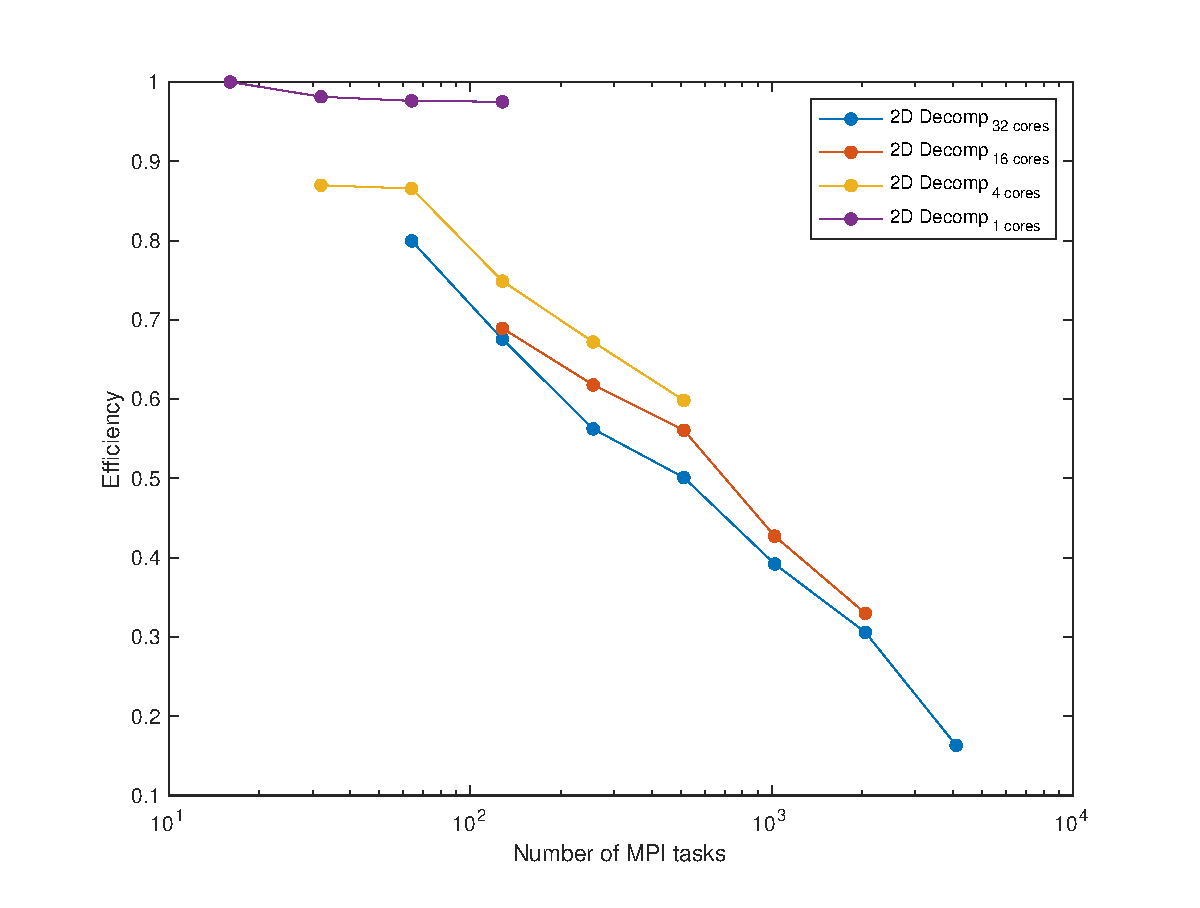
\includegraphics[scale=0.6]{grafici/20484}
\caption{Efficiency factor of $4096\times512 \times256$ simulation using 2D decomposition}
\label{20484}
\end{center}
\end{figure}
Increasing the counter of threads per processor leads to constant losses, as expectable. However, such losses between adjacent stations are lower than the ones of the previous simulations, furthermore we can see wider gaps among the efficiency curves, symptom that there is wider room for improvements.\par
Moreover, at very high number of cores, the efficiency curves slope is minor than before, preserving efficiency and allowing us to perform faster computations with greater speedups.\\
\par
To talk about speedups is useful to introduce figure~\ref{20482}, in which these are reported.\par
The graph, on page~\pageref{20482}, shows the results achieved by the 1D and 2D domain decomposed algorithm, with emphasis on the effects of the variation of cores per processor quantity, for the 2D algorithm only.\par
As has been done in the previous section, the high efficiency shown by the single core run, combined with the physical impossibility to use less cores, has lead us to made the assumption of speedup equal to 16 for a 16 parallel processes run in a single core environment.All other efficiencies and speedups have been derived using such data as reference.\\
\par

\begin{table}
\caption{Data from $4096\times 512\times 256$ simulation, 2D decomposition}
\begin{center}
\begin{tabular}{c c c c c}
\toprule
\textbf{\#Processes} & \textbf{Time [s]} & \textbf{Speedup} & \textbf{Efficiency [\%]} & \textbf{cores}\\
\midrule
16 & 1121.5 & 16 & 100 & 1\\
\hline
\multirow{2}{*}{32} & 571.4 & 31.4 & 98 & 1\\
& 644.8 & 27.83 & 87 & 4\\
\hline
\multirow{3}{*}{64} & 287.2 & 62.47 & 98 & 1\\
& 323.9 & 55.39 & 87 & 4\\
& 350.7 & 51.17 & 80 & 16\\
\multirow{4}{*}{128} & 143.8 & 124.8 & 98 & 1\\
& 187.2 & 95.85 & 75 & 4\\
& 203.4 & 88.23 & 69 & 16\\
& 207.5 & 86.47 & 68 & 32\\
\hline
\multirow{3}{*}{256} & 104.3 & 172 & 67 & 4\\
& 113.4 & 158.2 & 62 & 16\\
& 124.6 & 144 & 56 & 32\\
\hline
\multirow{3}{*}{512} & 58.6 & 306.4 & 60 & 4\\
& 62.5 & 287.1 & 56 & 16\\
& 70 & 256.5 & 50 & 32\\
\hline
\multirow{2}{*}{1024} & 41 & 437.5 & 43 & 16\\
& 44.7 & 401.4 & 39 & 32\\
\multirow{2}{*}{2048} & 26.6 & 675.5 & 33 & 16\\
& 28.7 & 626.3 & 31 & 32\\
\hline
4096 & 26.8 & 668.8 & 16 & 32\\
\bottomrule
\end{tabular}
\end{center}
\label{2048:data:2}
\end{table}

As can be seen in table~\ref{2048:data:2} the best result is achieved using 16 cores per processor and 2048 parallel processes. Unfortunately, due to some policy limitations, we can not push forward our resources request, although the graph clearly shows margins of improvements for such configuration.\\
\par
Differently from all the previous simulations, the processor grid for the pencil decomposition results balanced when the streamwise stencil has half the modes with respect to the other direction. Such configuration has been suggested by benchmarks.
\par
In conclusion we may say that, although the modes distribution results unbalanced in this simulation, the speedup trend still remain aligned with the ones exhibited in the other simulations.
\begin{figure}
\begin{center}
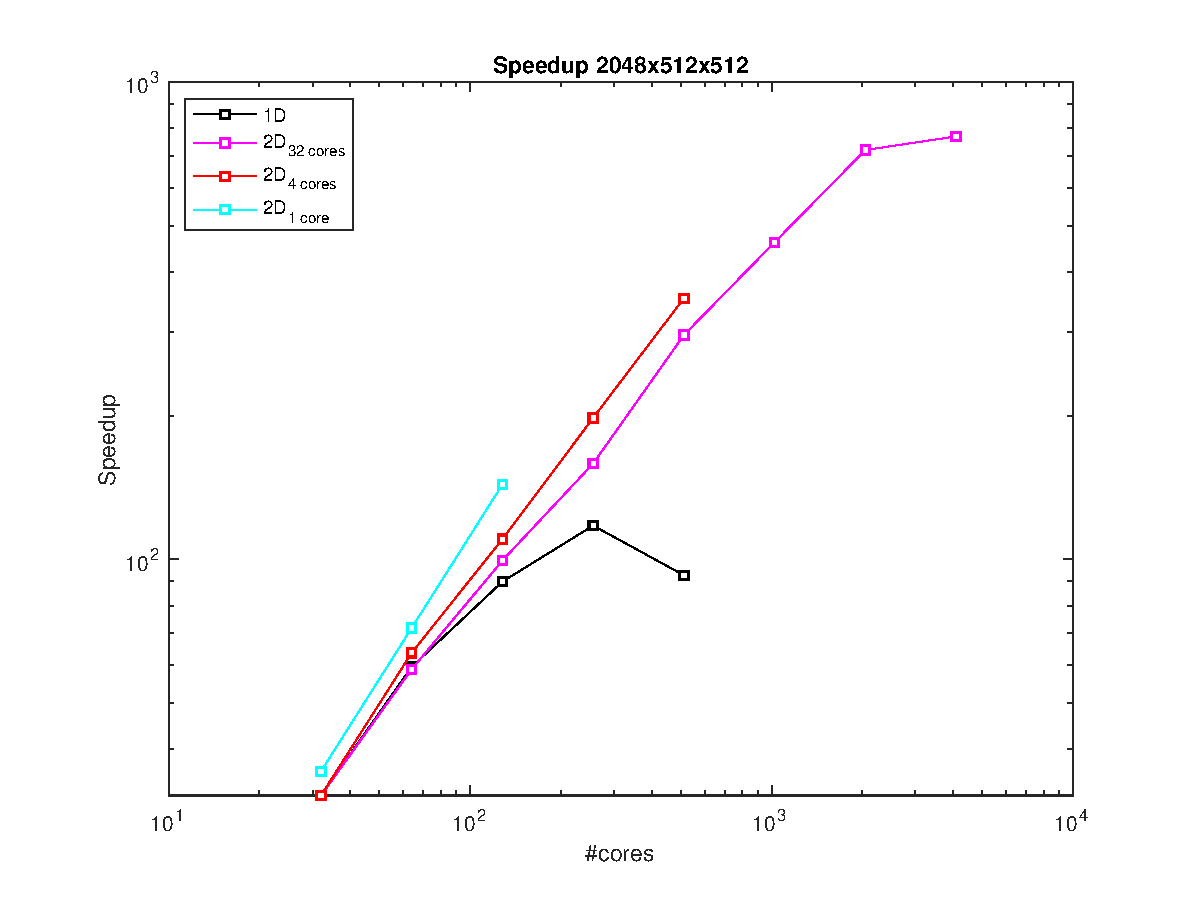
\includegraphics[scale=0.6]{grafici/20482}
\caption{Speedup factor of $4096\times512 \times256$ simulation}
\label{20482}
\end{center}
\end{figure}





\section{Benchmarks conclusions}
The benchmark series has highlighted common trends present in our simulations.
\par
By looking at the curves, we can see that the performances envelope is bordered by the 64 cores run and the single core ones.  We can catch from the graphs that the code tends to perform faster using as less threads per processor as possible.  This behavior is reasonable, since our code and the library in which we rely on to perform the MPI transposition, does not implement the OpenMP technology at the moment, so, although we could carry on the simulation basing our communications on MPI, we will experience efficiency lacks when dealing with intra-node messagings. In particular, when dealing with many cores per processor we face a speedup tendency to pass from 2 to $2^{2/3}$, as the number of MPI tasks gets doubled, as highlighted in~\cite{dns:gpu:supercomputer}. \par
Unfortunately, the Intel KNL's architecture~\cite{intel:xeonphi} is designed to exploit code vectorization as much as possible and OpenMP plays a key role in this kind of implementations. \par
We suggest to move to traditional processors architectures, instead of using MIC, to experience lower losses. Our simulations in fact has highlighted that, although MPI can not guarantee high efficiency in heavily threaded applications, the lacks using 16 cores, or less, per processor can be acceptable.\\
\par
As the problem size grows, the optimal number of MPI tasks, to achieve the best speedup, grows. In fact, we passed from 512 parallel processes for a $128^{3}$ simulation to 2048 for a $512^{3}$ simulation. \par

\begin{figure}
\begin{center}
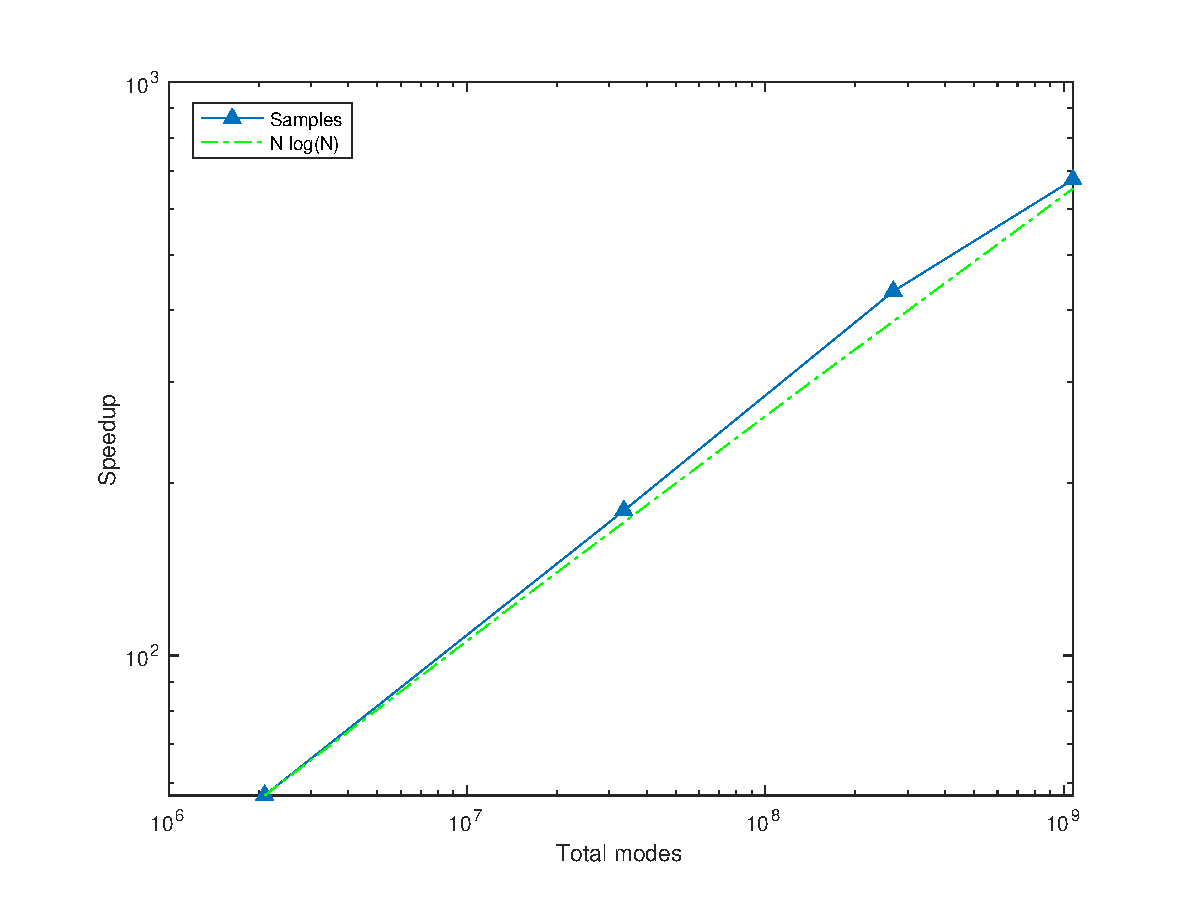
\includegraphics[scale=0.6]{grafici/speedup_trend}
\caption{Speedup factors growth}
\label{speedup:trend}
\end{center}
\end{figure}

On the other hand, the speedup factor increase its peak in a fashion which lies between $N\log(N)$ and $N^{2}$, like testify by figure~\ref{speedup:trend} in which our samples are plotted against such behaviors. \\
\par

\begin{figure}
\begin{center}
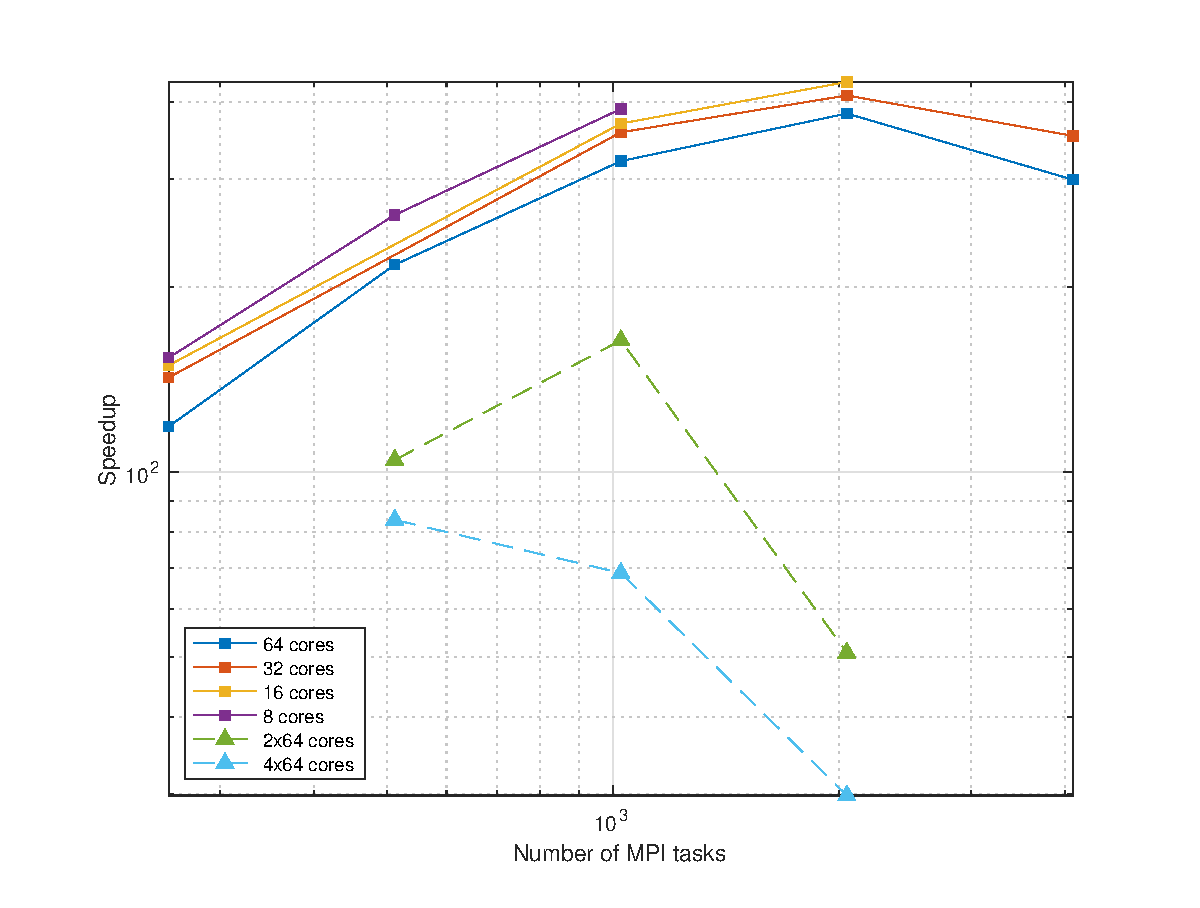
\includegraphics[scale=0.6]{grafici/hyperthreading}
\caption{Hyper threading benchmark}
\label{hyper}
\end{center}
\end{figure}

In conclusion we show the speedup comparison with hyper threading turned on. \par
Hyper threading is a technology~\cite{hyper:paper} developed by Intel that virtually doubles the cores on the CPU, making the CPU run faster and more efficient by scheduling the workload between the cores. On modern Xeon Phi we can quadruplicate the number of cores, obtaining until 272 threads per processor. However, as our benchmark shows, this technology does not provide a boost in terms of speedup, on the contrary it penalizes our results in evident fashion.\par
In figure~\ref{hyper} are compared the original results of a $512^{3}$ simulation, running on different cores per processor, against two curves which exploit the hyper threading technology.

\chapter{Simulations Results} 
\section{$Re_{\tau}=180$ simulation} \label{chapter:Re180}

The $Re_{\tau}=180$ simulation has been used to validate our results against the~\cite{kim_moin_moser} ones. \par

The channel length is $4\pi \delta$, while the width is $2 \pi \delta$, with $\delta$ indicating the half channel height. \par
Since our code employ spectral decomposition along the $xy$ plane, we define the streamwise and spanwise periods as $L_{x}= 2\pi /\alpha_{0}$ and $L_{z}=2\pi /\beta_{0}$, with $\alpha_{0}$ and $\beta_{0}$ fundamental wavenumbers. \par
The simulation take place using constant pressure gradient, imposed along $x$ direction, therefore $meanpx=1$.\par
The mesh along $y$ direction is non-uniform, discretized as
\begin{equation*}
y(i)=y_{min}+\frac{1}{2}(y_{max}-y_{min})  \frac{\tanh(a(2i/ny-1))}{\tanh(a)+0.5(y_{max}-y_{min})}
\end{equation*}
with $a=1.6$.\par
The timestep is constant, with $dt=0.0001$ and the simulation time is $T=50$ non dimensional units.
The grid employ 96 modes along $x$ dimension, which, thanks to the Hermitian symmetry, behave as 192 points. The $y$ is discretized using 128 points, while, along the $z$ direction, we have 160 points. The total mesh size reach approximately 2 millions of grid points, decomposed across 512 cores, employed during the simulation. 

The domain and the details about the simulation are summarized in table~\ref{table:180}.\\~\par
\begin{table}[h]
\caption{Simulation data for $Re_{\tau}$=180}
\begin{center}
\begin{tabular}{ccccccccccccc}
\toprule
$L_{x}$ & $L_{z}$ & $\delta$ & $nx$ & $nz$ & $ny$ & $\alpha_{0}$ & $\beta_{0}$ & $\Delta x^{+}$ & $\Delta z^{+}$ & $px$ & $dt$ & $T$\\
$4\pi$ & $2\pi$ & 1 & 192 & 160 & 128 & 0.5 & 1 & 11.8  & 7 & 1 & 0.0001 & 50 \\
\bottomrule
\end{tabular}
\end{center}
\label{table:180}
\end{table}

The bulk mean velocity, defined as 
\begin{equation}
\label{bulk:velocity}
U_{m} = \int_{0}^{1} \bar{u}d \big(\frac{y}{\delta} \big)
\end{equation}

normalized by the wall-shear velocity, is 15.66, which gives the Reynolds number based on the bulk mean velocity and the full channel width, $Re_{b}\approx 5600$. \\~\par
The graphs~\ref{loglaw_180} and~\ref{budget_180} show the behavior of the mean velocity and the roots means squares in the near wall region, with $\bar{u}$ indicating the mean velocity profile. \par
In both figures we reported the \emph{Kim et al.} results, using dotted line, for comparison. \\~\par

\begin{figure}
\begin{center}
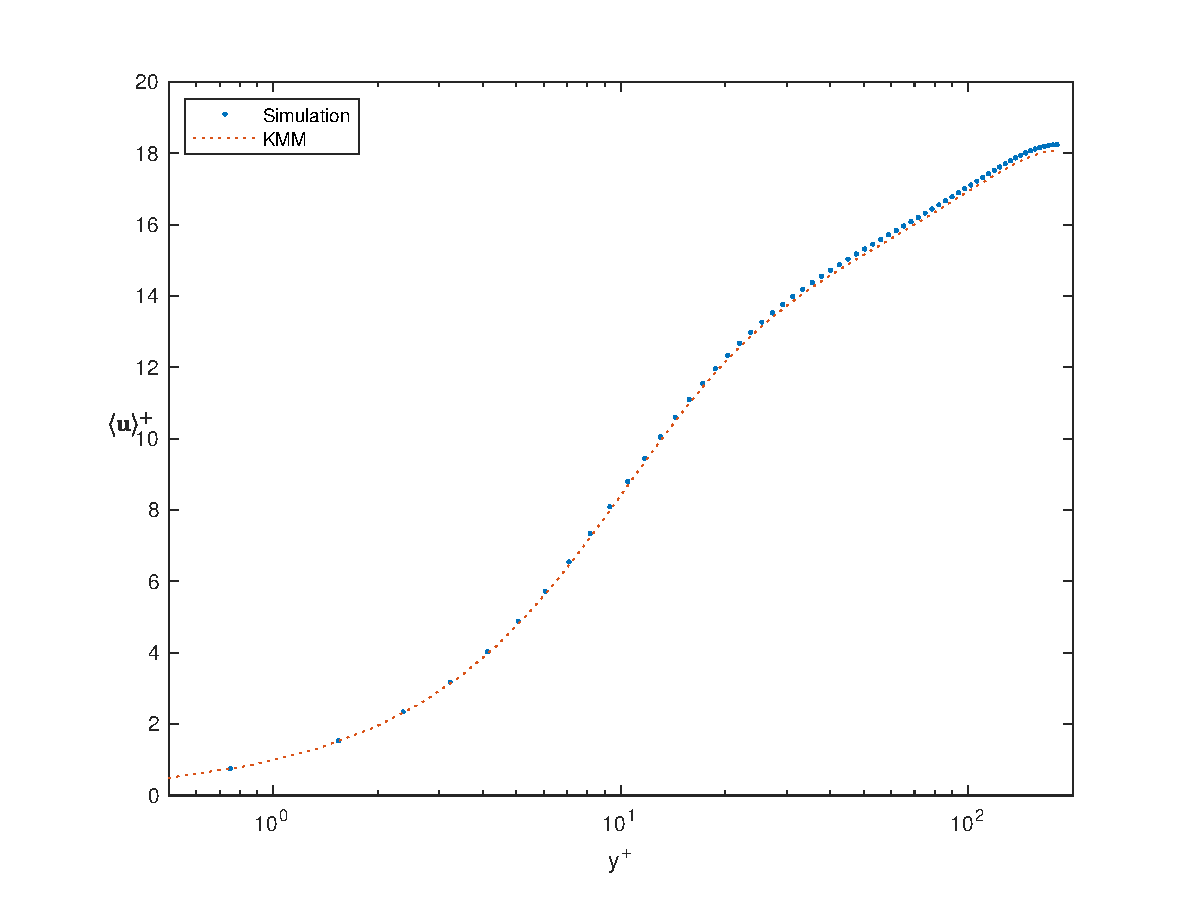
\includegraphics[scale=0.55]{grafici/loglaw_180.eps}
\caption{$\bar{u}^{+}$ in the near wall region for a $Re_{\tau}=180$ simulation}
\label{loglaw_180}
\end{center} 
\end{figure}
\begin{figure}
\begin{center}
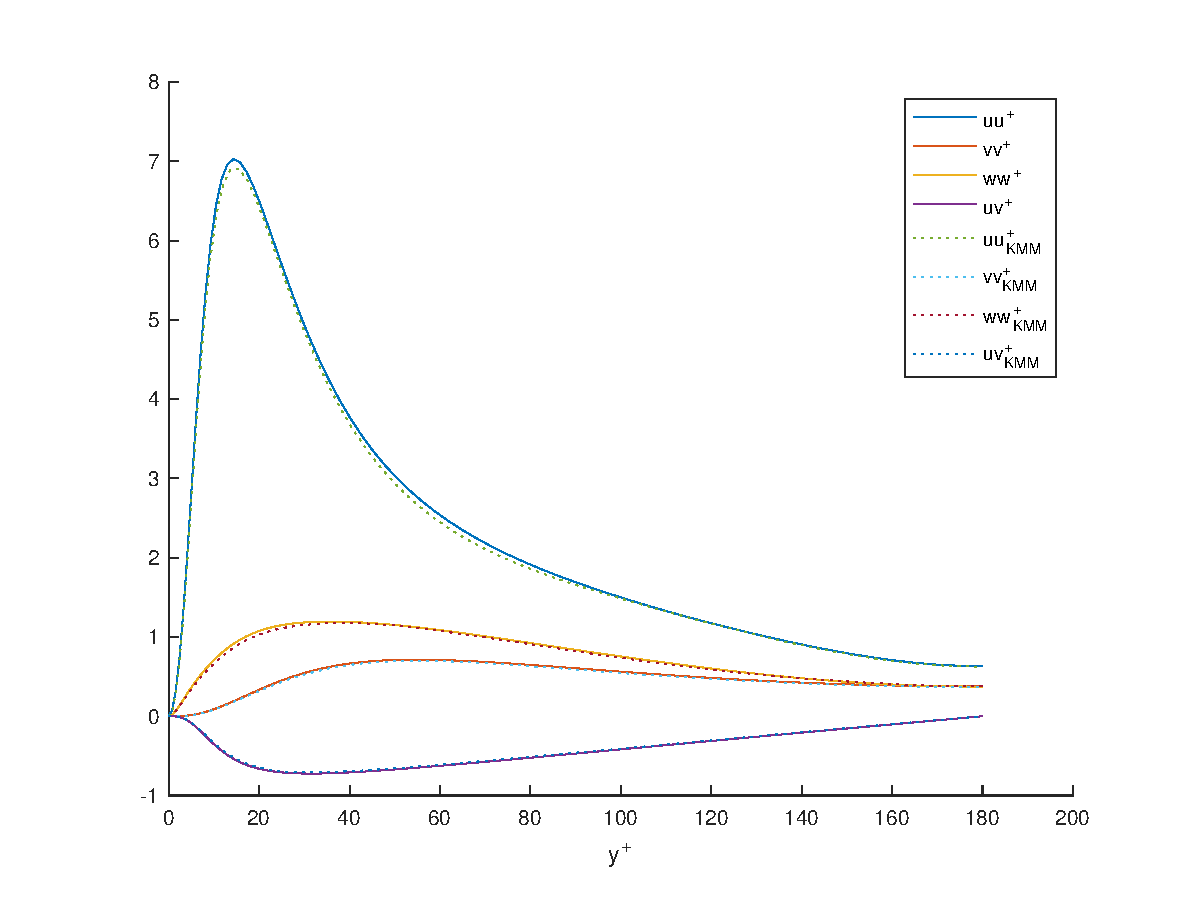
\includegraphics[scale=0.55]{grafici/budget_180.eps}
\caption{\emph{rms} terms for a $Re_{\tau}=180$ simulation}
\label{budget_180}
\end{center} 
\end{figure}


Our statistics have been registered using a simulation time of 50 non dimensional units, sampling data every 0.1 steps.
In total 500 fields have been used to perform the ensemble average. \par

The data fitting is good, despite being perfect. The divergences among our database and the~\cite{kim_moin_moser} ones are possibly due to the fluctuations, rounding errors and differences in averaging times.\\~\par

Nevertheless the results are in agreement with the typical curves behavior, in particular, by looking at the root mean square curves, we can clearly see that $\langle uu\rangle$ and $\langle ww\rangle$ depart from 0 as $y^{2}$, while $\langle uv\rangle$ and $\langle vv\rangle$ increase more slowly, as $y^{3}$ and $y^{4}$, in agreement with~\cite[284]{pope}.
All these information testify that, close to the walls, there is a \emph{two component flow}, with $v=0$ whereas $u$ and $w$ are non-zero. The resulting motion corresponds to flow in planes parallel to the wall. \\~\par

The figure~\ref{loglaw_180} report the $\bar{u}$ behavior near the wall. From 0 up to 5 $y^{+}$ units we can see the typical $\bar{u}=y^{+}$ behavior, which characterize the viscous sublayer. Once $y^{+}>30$ we see the arise of the logarithmic law of the wall, characterized by the equation

\begin{equation*}
\bar{u}^{+} = \frac{1}{\kappa} \ln y^{+} +C^{+},
\end{equation*}


\begin{figure}
\begin{center}
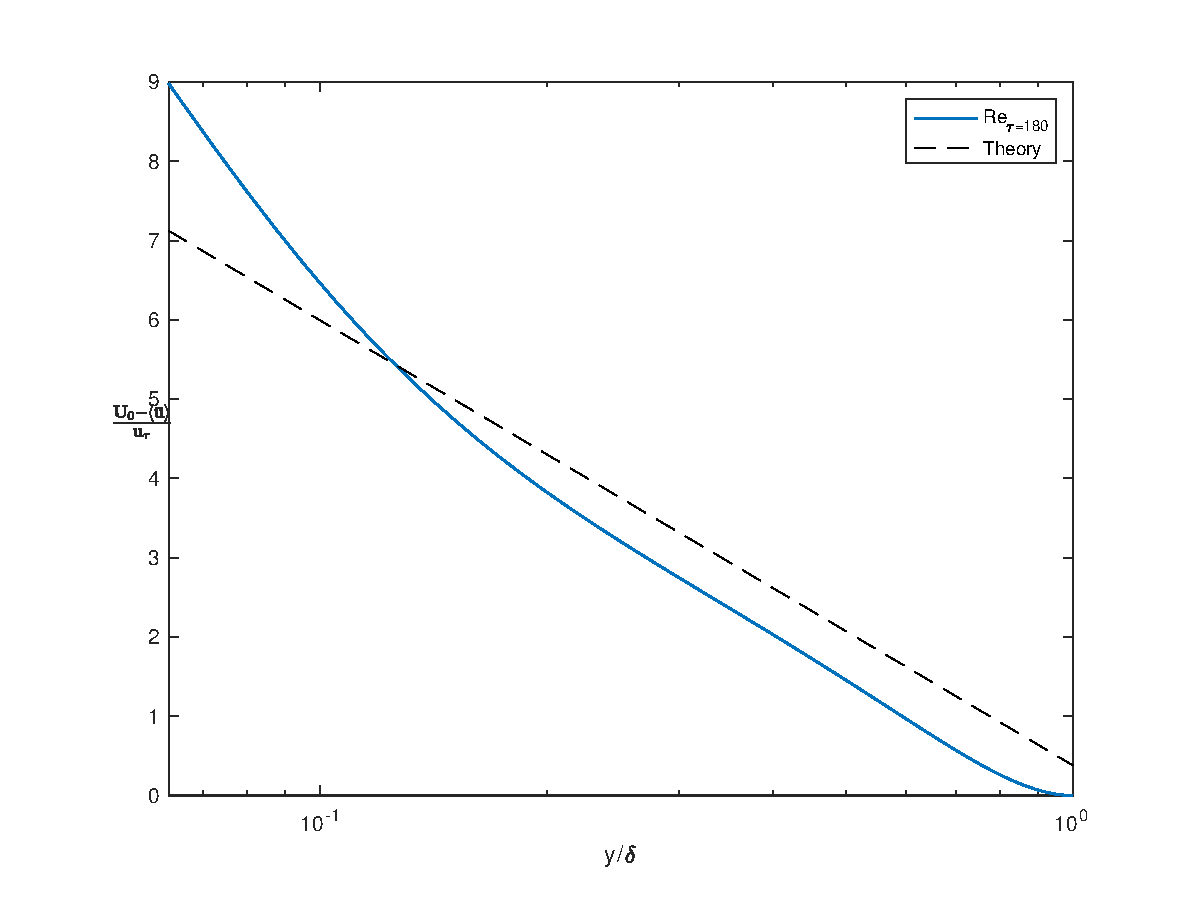
\includegraphics[scale=0.55]{grafici/velocity_defect_180.eps}
\caption{Velocity defect for a $Re_{\tau}=180$ simulation}
\label{velocity:defect:180}
\end{center} 
\end{figure}

where the constants $\kappa=0.41$ and $C^{+}\approx 5.2$, like smooth wall experiments, made by Von Karman, evidenced. \par
This velocity profile is typically denoted as \emph{the law of the wall}, and has been postulated by Prandtl in 1925.\par
Far away from the wall, the implications of the previous law originate the so called \emph{velocity defect}.
Our experimental data fits the theory, as figure~\ref{velocity:defect:180} suggest.\\~\par

The turbulence intensity trend reported on figure~\ref{rms:kmm:180} shows the comparison between the \emph{rms}, normalized by $u_{\tau}$, obtained by \emph{Kim et al.} and our results, plotted against the wall-normal distance $y^{+}$. 
The fitting is good, particularly by approaching the centerline.\par

The maxima are located between the outer region of the buffer layer and the beginning of the log-law region: the streamwise $u'/u_{\tau}$ peak is positioned at $y^{+} \approx 14$ with a value of $u'/u_{\tau} \approx 2.65$. The other two components show a smoother and less prominent behavior, with a $w'/u_{\tau} \approx 1.08$ around $y^{+} \approx 38$ and $v'/u_{\tau} \approx 0.84$ for $y^{+} \approx 50$. \\~\par

\begin{figure}
\begin{center}
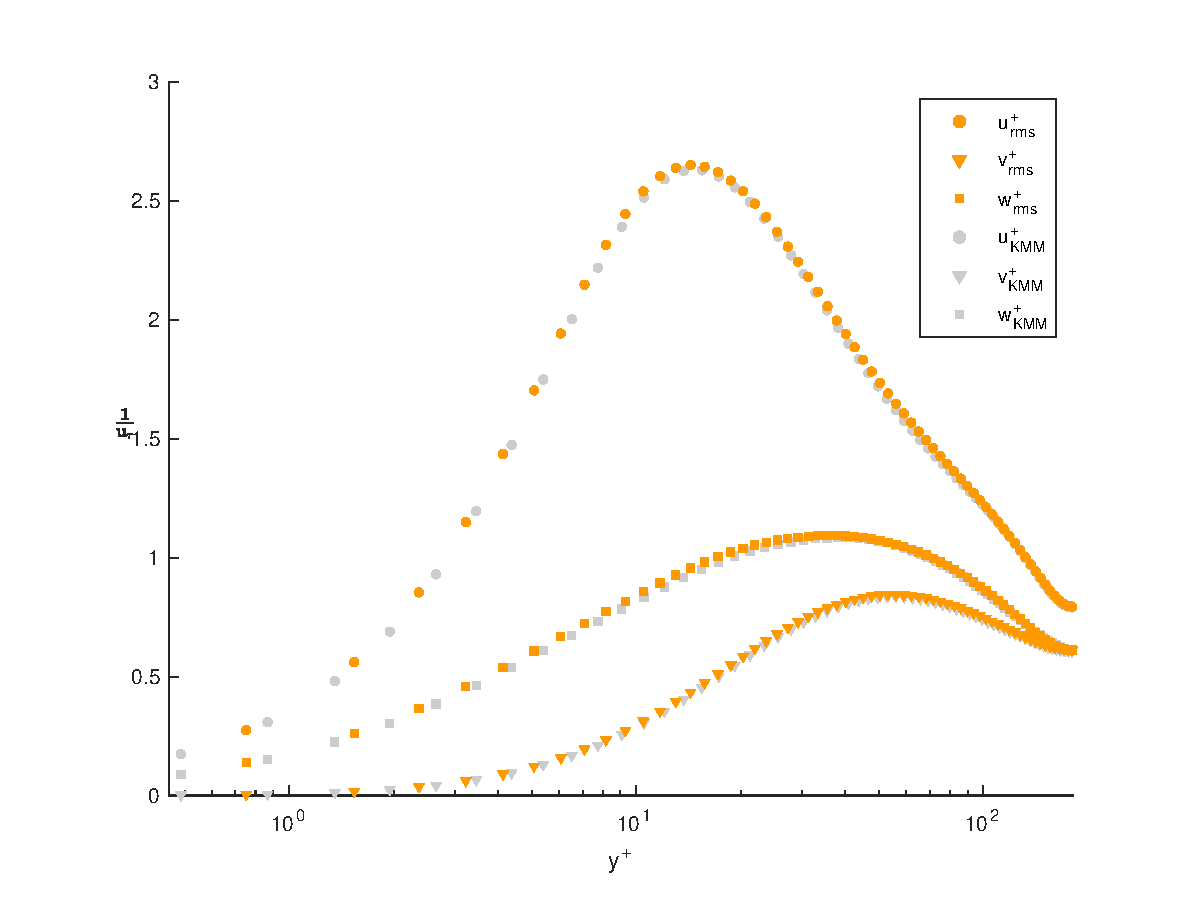
\includegraphics[scale=0.55]{grafici/rms_kmm.eps}
\caption{\emph{rms} behavior on a $Re_{\tau}=180$ simulation}
\label{rms:kmm:180}
\end{center} 
\end{figure}

A deeper knowledge of what happen close to the wall can be obtained by looking at figure~\ref{wall:rms:180}.
Such picture shows the behavior of the three \emph{rms} components, normalized by the wall coordinate, for the first 9 wall units. In dashed line it is possible to see the data from \emph{Kim et al.} \par
Once again the fitting between data is good, with both curves that follow the same trends.
It is interesting to show that for the first wall units, in the viscous sublayer, the ratio $u'/y^{+}$ remains constant, indicating constant turbulence generation. It is quite flat also the $w'/y^{+}$ behavior, while the $v'/y^{2+}$ exhibit a more slope trend.\par
The last curve is not in scale, the graph, indeed, shows a 10x magnified value, just for plotting purpose.\\~\par

\begin{figure}
\begin{center}
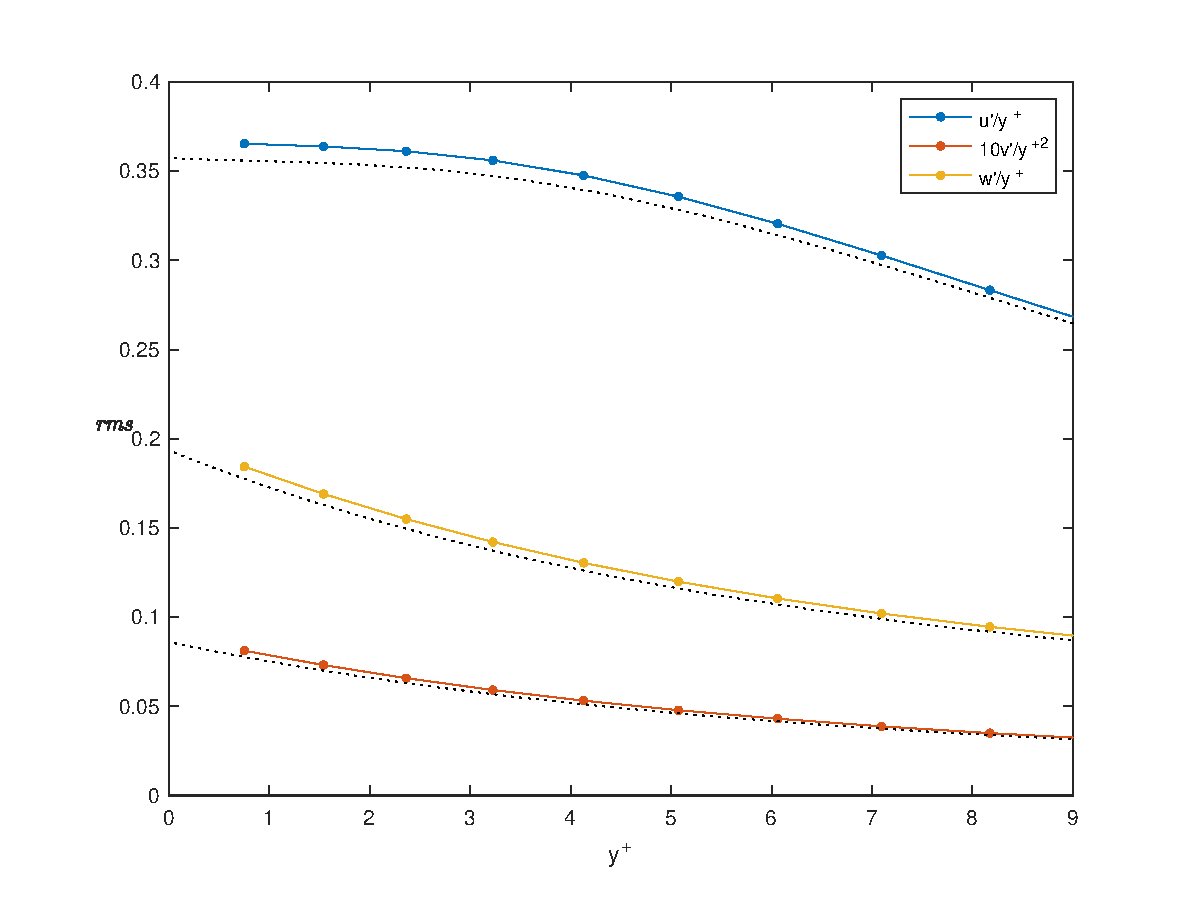
\includegraphics[scale=0.55]{grafici/wall_rms_180.eps}
\caption{Normalized \emph{rms} close to the wall for a $Re_{\tau}=180$ simulation}
\label{wall:rms:180}
\end{center} 
\end{figure}

On page~\pageref{k+budgets:180} is possible to look at the plot of the turbulent kinetic energy with the \emph{rms} terms, while figure~\ref{tke:prod:180} shows the \emph{production term}, defined as $P=-\langle u'v'\rangle \partial{\bar{u}}/\partial{y}$.\par
The two images highlight that the energy associated with the turbulence tends to develop close to the walls, and lose effectiveness once departing from there.\par
The \emph{production term} is part of the so called turbulent kinetic energy budgets and plays a key role in the interaction of the mean energy equation and TKE. The action of the mean velocity gradients working against the Reynolds stresses removes kinetic energy from the mean flow and transfers it to the fluctuating velocity field. \par
By looking at figure~\ref{tke:prod:180} we can clearly see that its contribution concentrated near the walls, with the peak around $y^{+} \approx 12$, and tends to become zero approaching the half channel height. \\~\par

\begin{figure}
\begin{center}
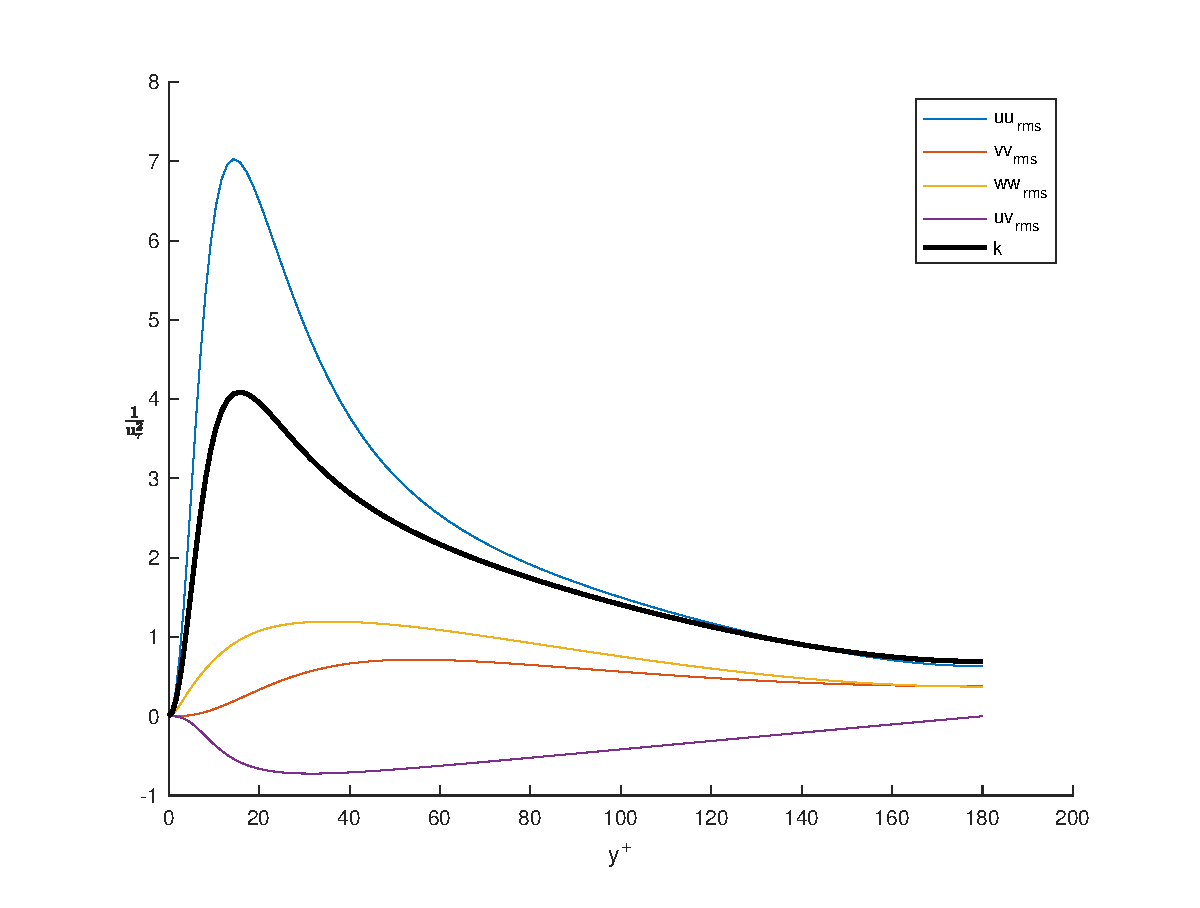
\includegraphics[scale=0.55]{grafici/budget+k_180.eps}
\caption{TKE and \emph{rms} terms for a $Re_{\tau}=180$ simulation}
\label{k+budgets:180}
\end{center} 
\end{figure}

\begin{figure}
\begin{center}
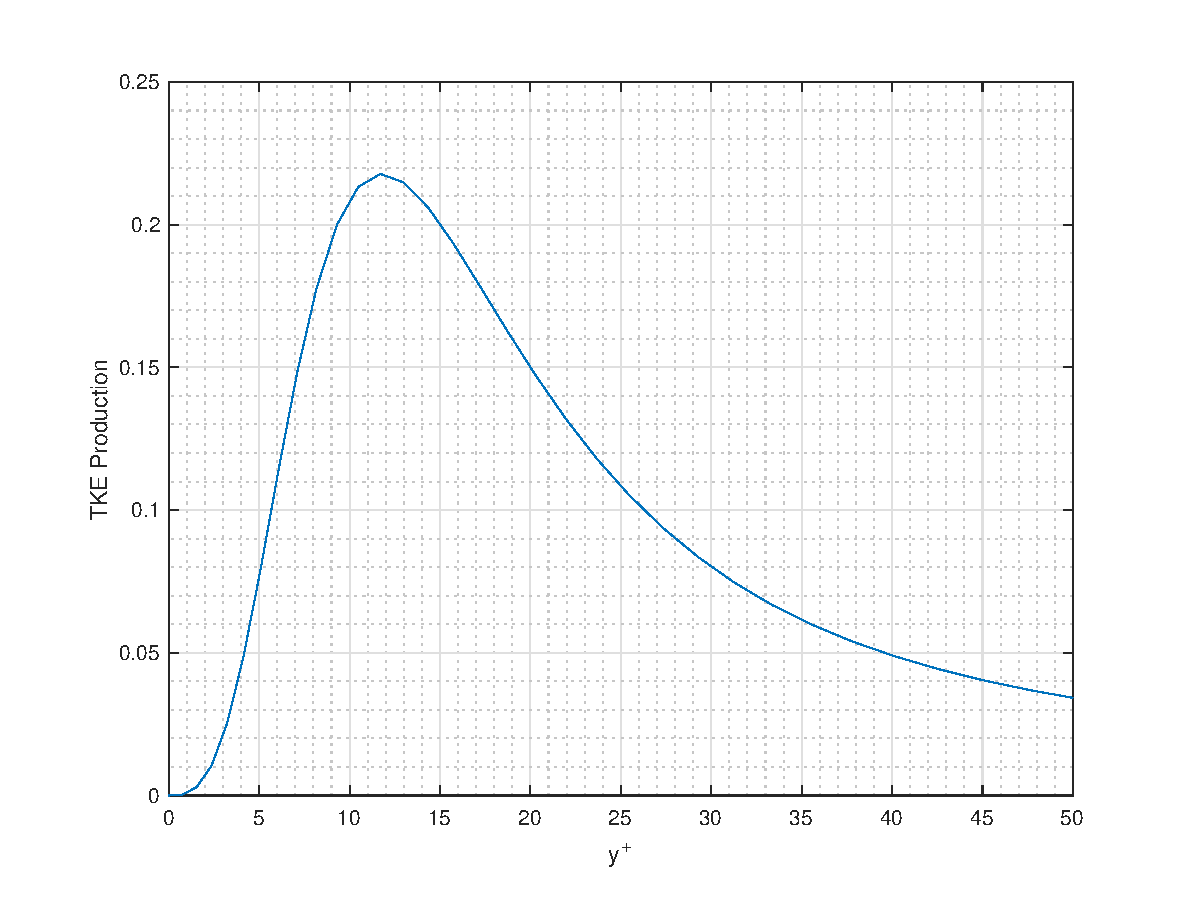
\includegraphics[scale=0.55]{grafici/tke_prod_180.eps}
\caption{Production term of the TKE eq. normalized by $Re_{\tau}=180$}
\label{tke:prod:180}
\end{center} 
\end{figure}

The \emph{production} peak occurs where the Reynolds stresses becomes equal to the viscous ones.
On figure~\ref{stresses:180} we reported the plot of the normalized total shear stress, with its contributions, in which we can see evidence of curves overlapping for $y\approx 12$.\par


\begin{figure}
\begin{center}
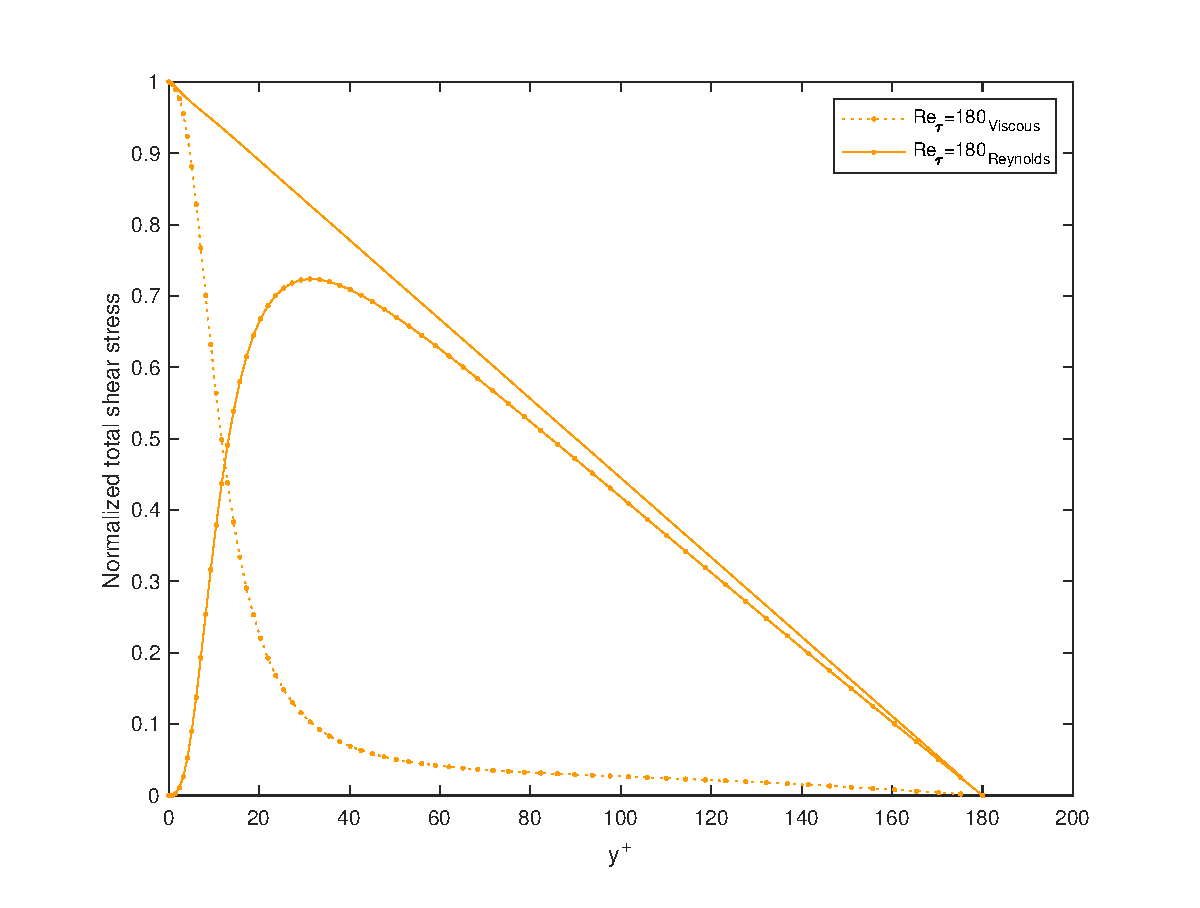
\includegraphics[scale=0.55]{grafici/stresses_180.eps}
\caption{Normalized total shear stress for a $Re_{\tau}=180$ simulation}
\label{stresses:180}
\end{center} 
\end{figure}
\section{$Re_{\tau}=1000$ simulation} 
The second simulation performed is carried out at $Re_{\tau}=1000$, which in terms of channel width and bulk velocity is equivalent to $Re_{b}\approx40000$.\par
The bulk velocity, obtained as shown in~\ref{bulk:velocity}, is 19.99, while $\alpha_{0}$ and $\beta_{0}$ are respectively 0.5 and 1, in order to reproduce the correct dimensions of the channel, as shown in chapter~\ref{chapter:Re180}.\par
Since the high computational cost needed to obtain these results we were unable to carry out a complete simulation. Thus the results reported shows the statistics associated with a flow in transitory phase. \\~\par

The simulation employed a variable timestep, determined through the Courant-Friedrichs-Lewy condition.
The CFL limit has been set to 1.6, close to the theoretical ones, equal to $\sqrt{3}$, for a third-order Runge-Kutta method. Such choice has been influenced by the high computational cost needed to compute the CFL. In fact, carry out such value requires three different transpositions and relative Fourier transformations. Therefore we decided to perform such computation approximately on every 10 steps. In this way the gain in terms of performance is significant, combining the flexibility of the Courant-Friedrichs-Lewy condition with a reduced cost to compute it.\par

The grid employed in this simulation face 500 points in the wall-normal direction, 2048 in the spanwise direction and 2048 points along the streamwise dimension, direction in which we exploit the Hermitian symmetry. According to this configuration, the grid size reach the billion of points.\par
Table~\ref{table:1000} report a summary of the simulation configuration for the $Re_{\tau}=1000$ case.\\~\par

\begin{table}
\caption{Simulation data for $Re_{\tau}$=1000}
\begin{center}
\begin{tabular}{ccccccccccccc}
\toprule
$L_{x}$ & $L_{z}$ & $\delta$ & $nx$ & $nz$ & $ny$ & $\alpha_{0}$ & $\beta_{0}$ & $\Delta x^{+}$ & $\Delta z^{+}$ & $px$ & $CFL$\\
$4\pi$ & $2\pi$ & 1 & 2048 & 2048 & 500 & 0.5 & 1 & 6.1  & 3 & 1 & 1.6 \\
\bottomrule
\end{tabular}
\end{center}
\label{table:1000}
\end{table}


Since are required approximately 50GB of disk space per each field we decided to avoid to save them on disk, instead we calculated the statistics runtime, merging the files at the end of the simulation, reducing the required space to few KB.\\~\par

The results that we will present shortly are obtained through the ensemble average of 100 fields, and cover 0.1 non dimensional time units. In this lapse of time the mean $Re_{\tau}$ is approximately 991 units.\par
Let us focus now on the statistics gained from the simulation.\\~\par
Figure~\ref{loglaw:1000} report the law of the wall. As we can see from the plot, made in semi-logarithmic scale using the wall units, our data fits the theoretical curve throughout the logarithmic region, while, towards the centerline, a residual sensitivity to the initial conditions is still present and lead to few differences with the results obtained by Moser \& Lee in~\cite{Lee}.\par
Far from the wall, the velocity defect law find good feedback with our results, as shown by the graph~\ref{velocity:defect:1000}.\\~\par

\begin{figure}
\begin{center}
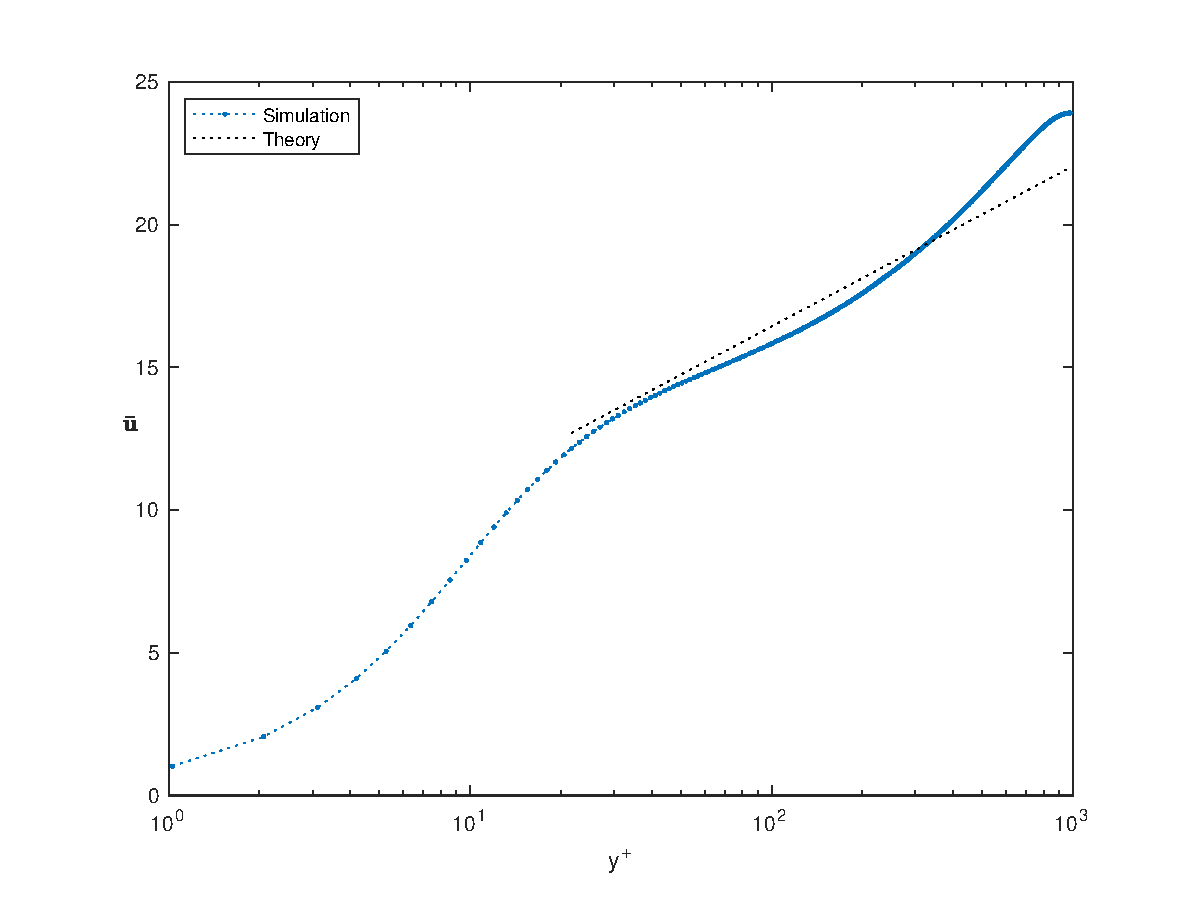
\includegraphics[scale=0.55]{grafici/loglaw_1000.eps}
\caption{$\bar{u}^{+}$ in the near wall region for a $Re_{\tau}=1000$ simulation}
\label{loglaw:1000}
\end{center} 
\end{figure}

\begin{figure}
\begin{center}
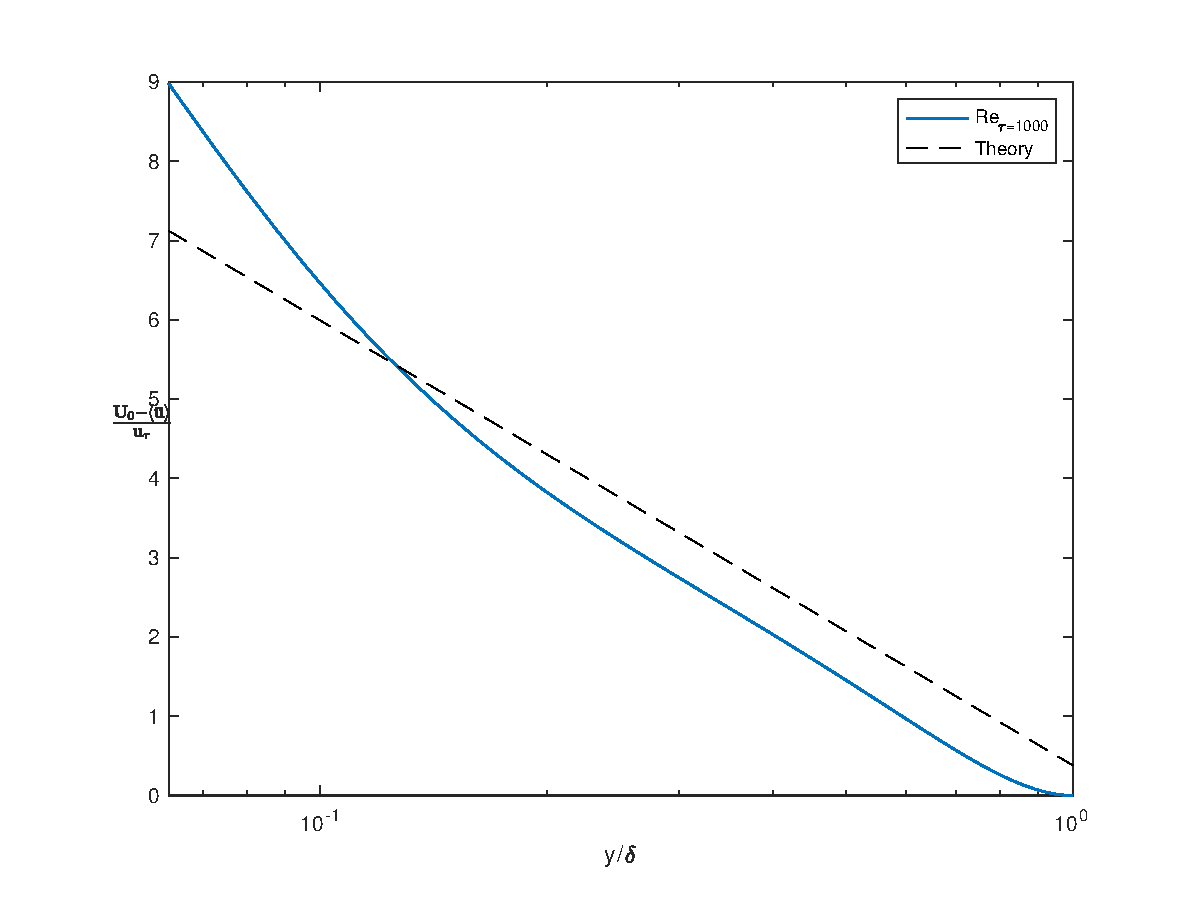
\includegraphics[scale=0.55]{grafici/velocity_defect_1000.eps}
\caption{Velocity defect for a $Re_{\tau}=1000$ simulation}
\label{velocity:defect:1000}
\end{center} 
\end{figure}

In figure~\ref{budget:1000} we reported the \emph{rms} fluctuations, normalized by the $u_{\tau}^{2}$, jointed with the TKE distribution. The first differences that we can immediately face by comparing our curves with the ones in figure~\ref{k+budgets:180} are the peak values. These values tends to increase with respect to the counterpart of the $Re_{\tau}=180$ simulation, highlighting how this simulation contains more energy than the previous ones.\par
Although there is an higher content of energy, the curves shape remains aligned with the ones seen in the previous chapter.\par
The near-wall behavior present a two-components turbulent flow. In fact, as evidenced by the magnification, the wall-normal fluctuations are absent for the first few units.
\\~\par

The production curve does not exhibit marked difference across the results of this simulation and the $Re_{\tau}=180$ simulation, as depicted in figure~\ref{tke:prod:1000}.\\~\par

\begin{figure}
\begin{center}
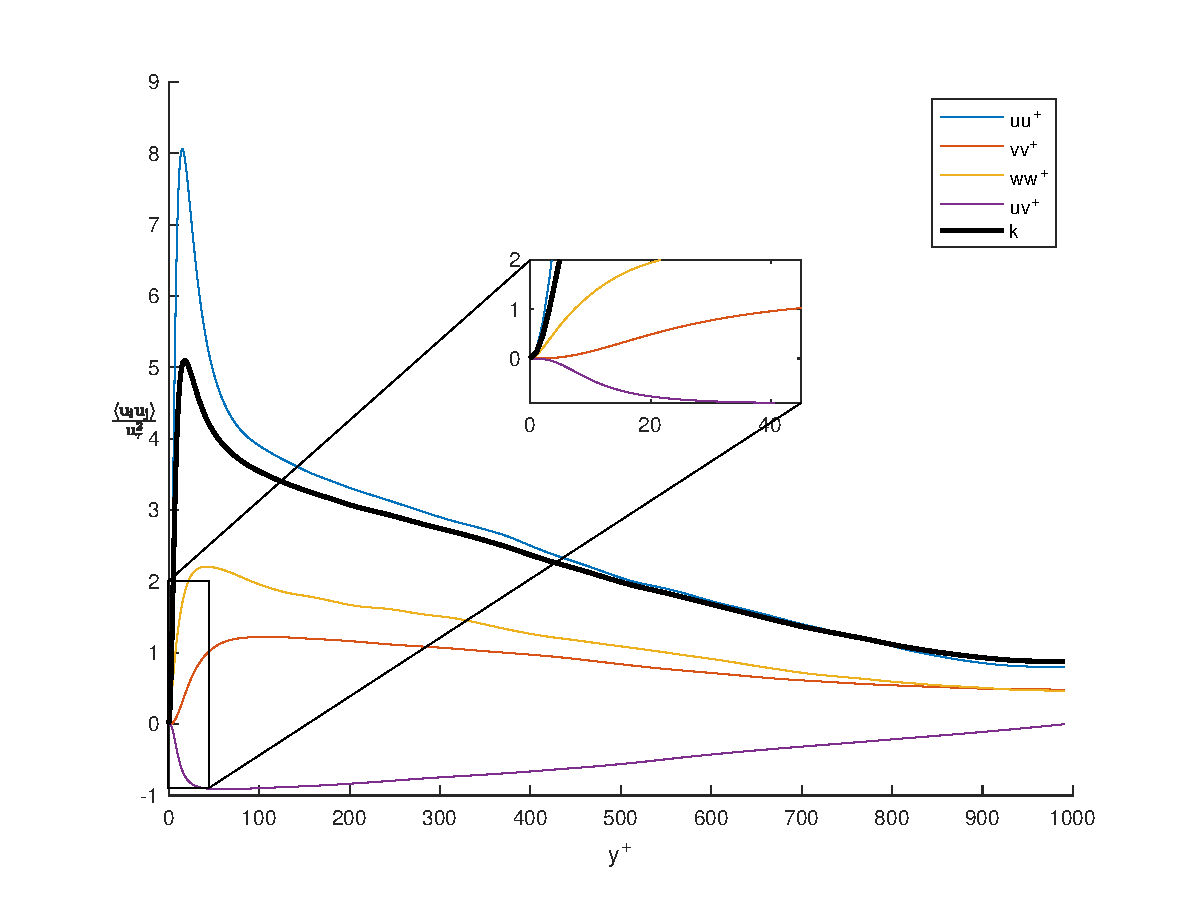
\includegraphics[scale=0.55]{grafici/budget+k_1000.eps}
\caption{\emph{rms} terms for a $Re_{\tau}=1000$ simulation}
\label{budget:1000}
\end{center} 
\end{figure}


The finer mesh and the higher Reynolds evidenced the appearance of a new turbulence peak, detached from the wall-cycle, identified through knees in the curves of figure~\ref{rms:1000}. \par
In such figure our results are compared with the ones of Moser \& Lee, which are the expected values for a complete $Re_{\tau}=1000$ simulation. \par
The results shows accordance among the expected values and the ones obtained through the simulation.
The $u'/u_{\tau}$ curve fits well the expect value, despite the little $Re_{\tau}$ difference among the two datasets.
The $v'/u_{\tau}$ and $w'/u_{\tau}$ curves are in good accordance with the values of Moser \& Lee in the inner region, while towards the centerline of the channel flow we face the raise of differences, due to the transitory nature of the simulation.\\~\par



\begin{figure}
\begin{center}
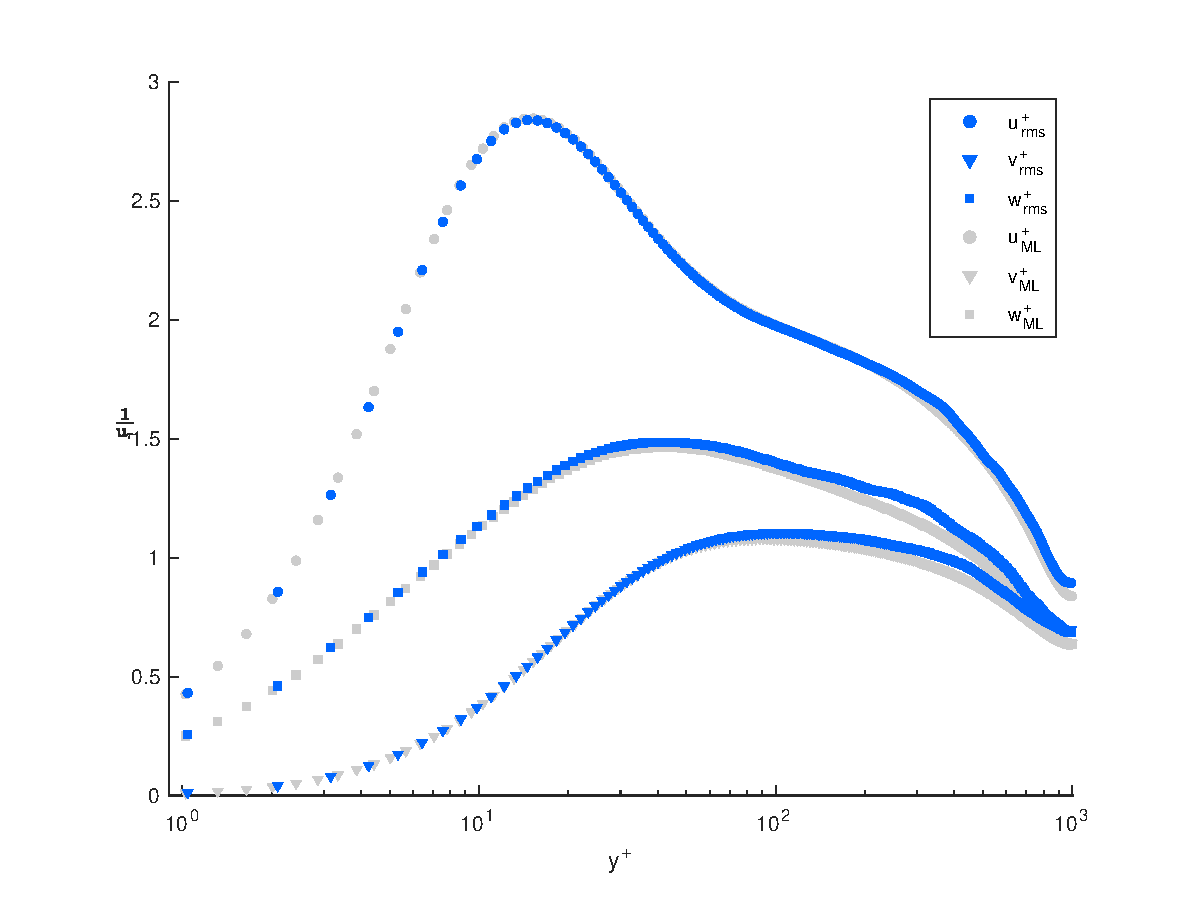
\includegraphics[scale=0.55]{grafici/rms_1000.eps}
\caption{\emph{rms} behavior on a $Re_{\tau}=1000$ simulation}
\label{rms:1000}
\end{center} 
\end{figure}

\begin{figure}
\begin{center}
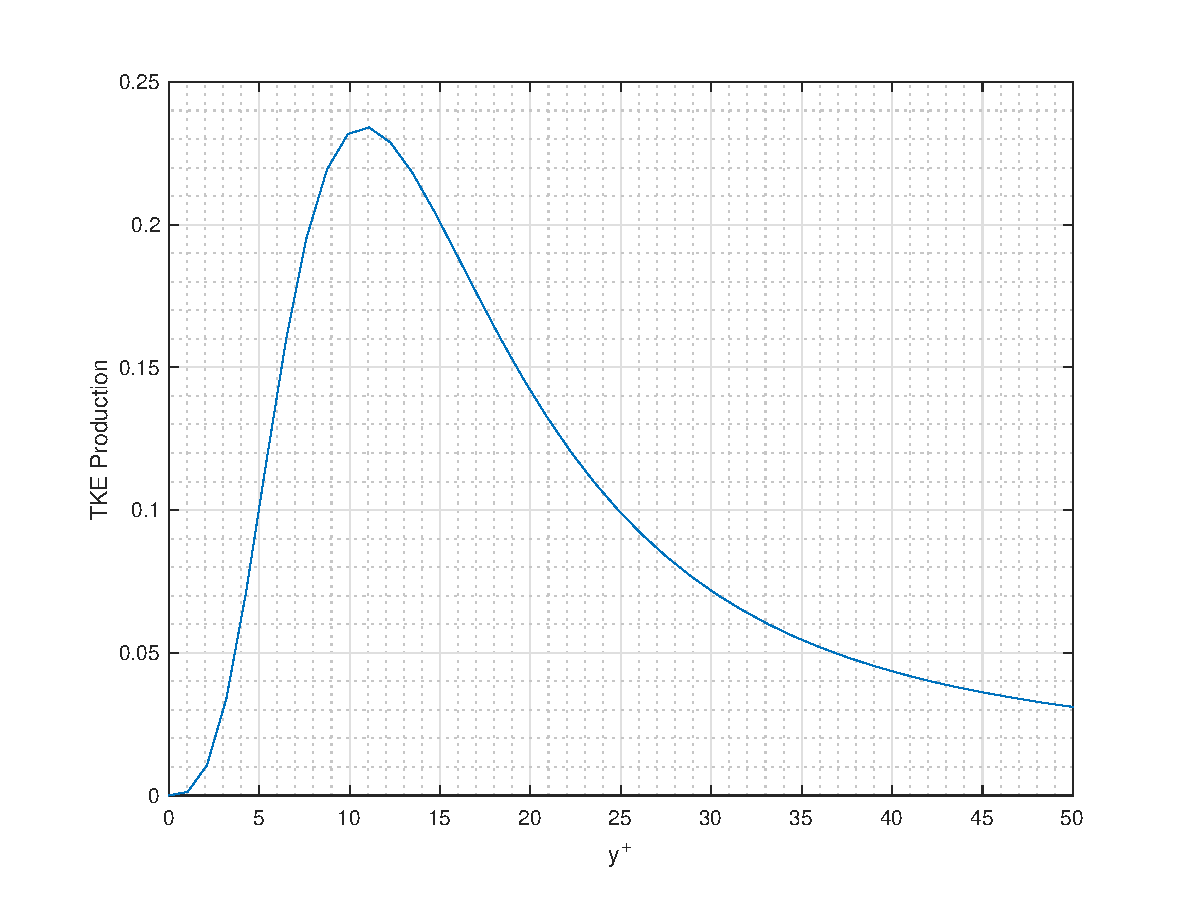
\includegraphics[scale=0.55]{grafici/tke_prod_1000.eps}
\caption{Production term of the TKE eq. for a $Re_{\tau}=1000$ simulation}
\label{tke:prod:1000}
\end{center} 
\end{figure}

Comparing the results of this simulation with the ones of the $Re_{\tau}=180$ we can clearly see a generalized upward shift of the \emph{rms} fluctuations. Such trend is present also near the wall. Indeed the curves does not exhibit marked changes in shape with respect to its counterpart in the previous simulation, as figure~\ref{wall:rms:1000} testify, just an upward shift, with the streamwise and spanwise components that depart from zero as $y^{+}$, while the wall-normal components leave the wall as $y^{2+}$. \\~\par

Similar reasoning applies also for the graphs of the \emph{production}, reported in figure~\ref{tke:prod:1000}, that reach a slightly higher peak of $P/Re_{\tau}=0.24$, without showing significant changes of the curve shapes. The peak is still located nearby $y\approx 12$.\\~\par

As theory affirms, the wall coordinate of the peak of production corresponds to that in which the stress components become equivalent. This aspect will be investigated further, comparing the results of all the simulations together.
At the present time we limit to illustrate the behavior of the stress components, which are reported in figure~\ref{stresses:1000}. As we can see, the normalized total shear stress is quasi-straight, suggesting that we are still in a transitory phase. The driving-train of this unsteadiness has to be searched in the excess of Reynolds stresses, which are forcing our flow towards higher Reynolds values. \par
\begin{figure}
\begin{center}
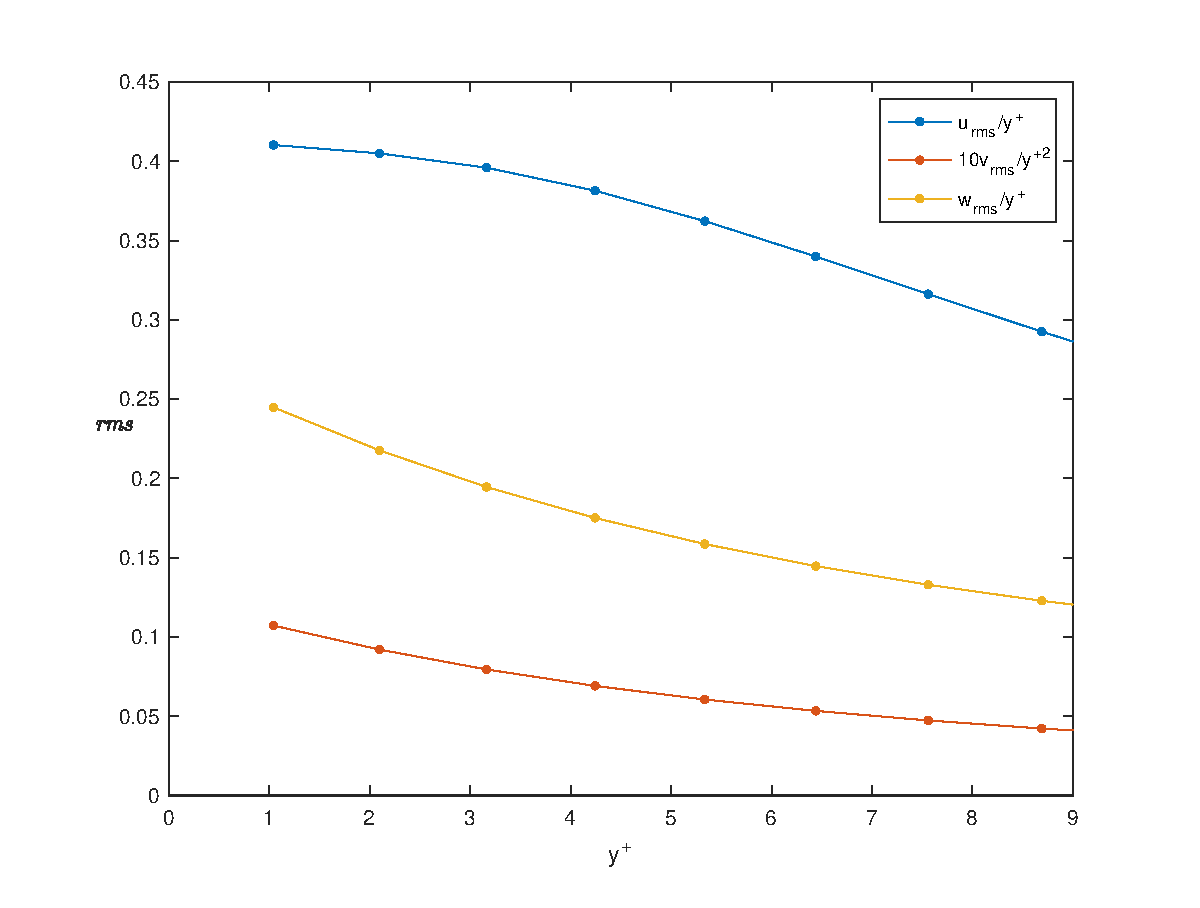
\includegraphics[scale=0.55]{grafici/wall_rms_1000.eps}
\caption{Normalized \emph{rms} close to the wall for a $Re_{\tau}=1000$ simulation}
\label{wall:rms:1000}
\end{center} 
\end{figure}

\begin{figure}
\begin{center}
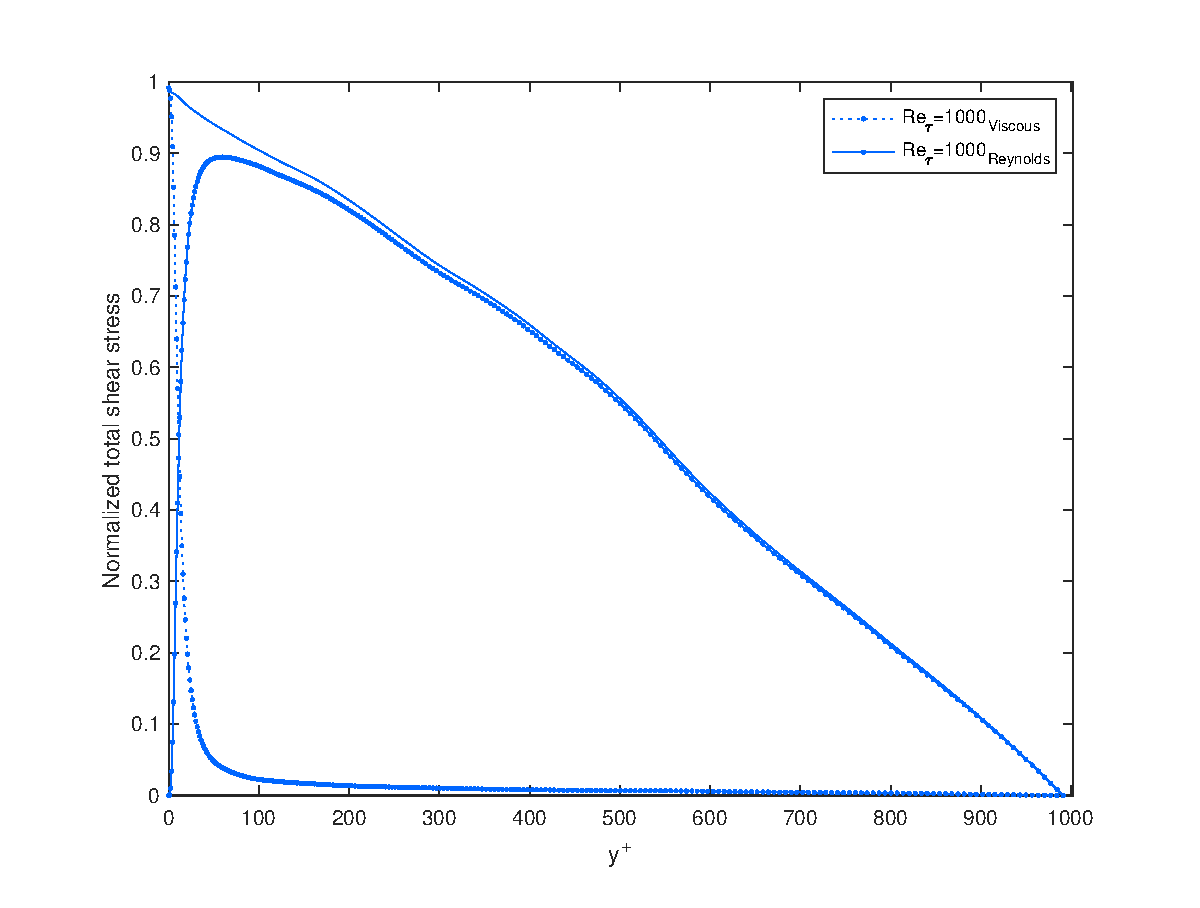
\includegraphics[scale=0.55]{grafici/stresses_1000.eps}
\caption{Normalized total shear stress for a $Re_{\tau}=1000$ simulation}
\label{stresses:1000}
\end{center} 
\end{figure}
\section{$Re_{\tau}=2000$ simulation} 
The last simulation performed is carried out at $Re_{\tau}\approx2000$, which in terms of channel width and bulk velocity is approximately equivalent to $Re_{b}=100000$.\par
The bulk velocity is 24.3, $\alpha_{0}$ is 0.5 and $\beta_{0}$ is equal to 1.\par
The timestep is variable, once again determined by the Courant-Friedrichs-Lewy condition set to 1, and the simulation time is T=0.01. \par
The excessive resource requests lead us to perform a reduced simulation, able just to highlight some of the main features of this $Re_{\tau}$, since the flow is still sensible to the initial conditions. Despite such reduced simulation time, in order to guarantee as better as possible results, we sampled the field every 0.001 steps, so that we can employ a 1000 fields to do the ensemble average.\\~\par
The grid employed in this simulation face 1000 points in the wall-normal direction, 4096 in the spanwise direction and 4096 points along the streamwise dimension. The mesh size is extremely huge, with more than 8 billions of points.\par
We reported a summary of the simulation configuration in table~\ref{table:2000}\\~\par

\begin{table}
\caption{Simulation data for $Re_{\tau}$=2000}
\begin{center}
\begin{tabular}{ccccccccccccc}
\toprule
$L_{x}$ & $L_{z}$ & $\delta$ & $nx$ & $nz$ & $ny$ & $\alpha_{0}$ & $\beta_{0}$ & $\Delta x^{+}$ & $\Delta z^{+}$ & $px$ & $CFL$ & $T$\\
$4\pi$ & $2\pi$ & 1 & 4096 & 4096 & 1000 & 0.5 & 1 & 6.1  & 3 & 1 & 1 & 0.01 \\
\bottomrule
\end{tabular}
\end{center}
\label{table:2000}
\end{table}


The disk space requirement raised approximately by a factor of 10, with 400GB of disk space needed per each field. This reason pushed us once again to rely in live post processing, instead of saving snapshots of the field.\\~\par

The statistics gained from the simulation are here presented.\par
We start from figure~\ref{loglaw:2000}, which report the law of the wall. Despite the graph is not perfect, during the simulation the data has shown a progressive tendency to re-align with the theoretical behavior, characterized by $k=0.41$ and $B=5.2$. As consequence, towards the centerline, the velocity defect law is affected by fluctuations caused by the poor temporal resolution, as shown by the graph~\ref{velocity:defect:2000}. Despite these fluctuations, it is possible to see that the region subject to linearity has become wider with respect to previous simulations. \\~\par

\begin{figure}
\begin{center}
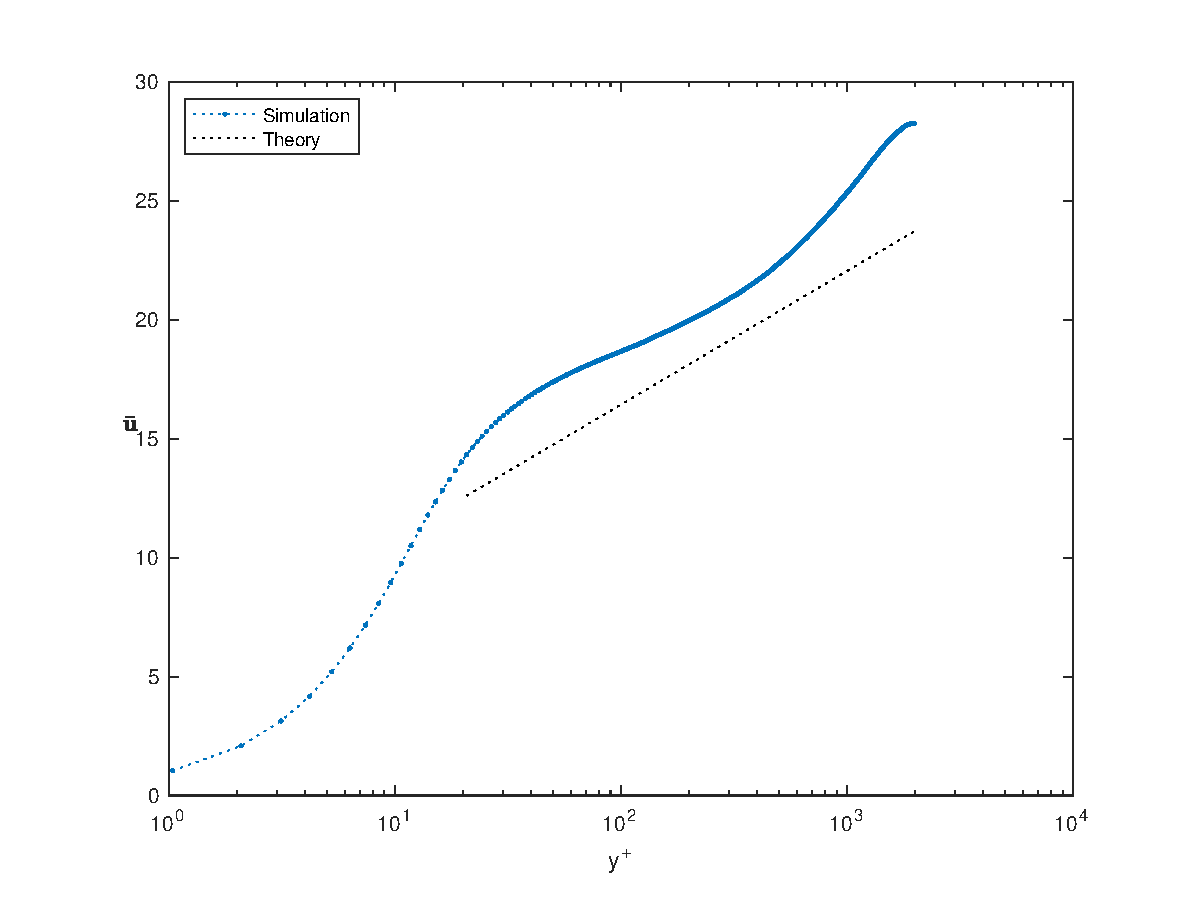
\includegraphics[scale=0.55]{grafici/loglaw_2000.eps}
\caption{$\bar{u}^{+}$ in the near wall region for a $Re_{\tau}=2000$ simulation}
\label{loglaw:2000}
\end{center} 
\end{figure}

\begin{figure}
\begin{center}
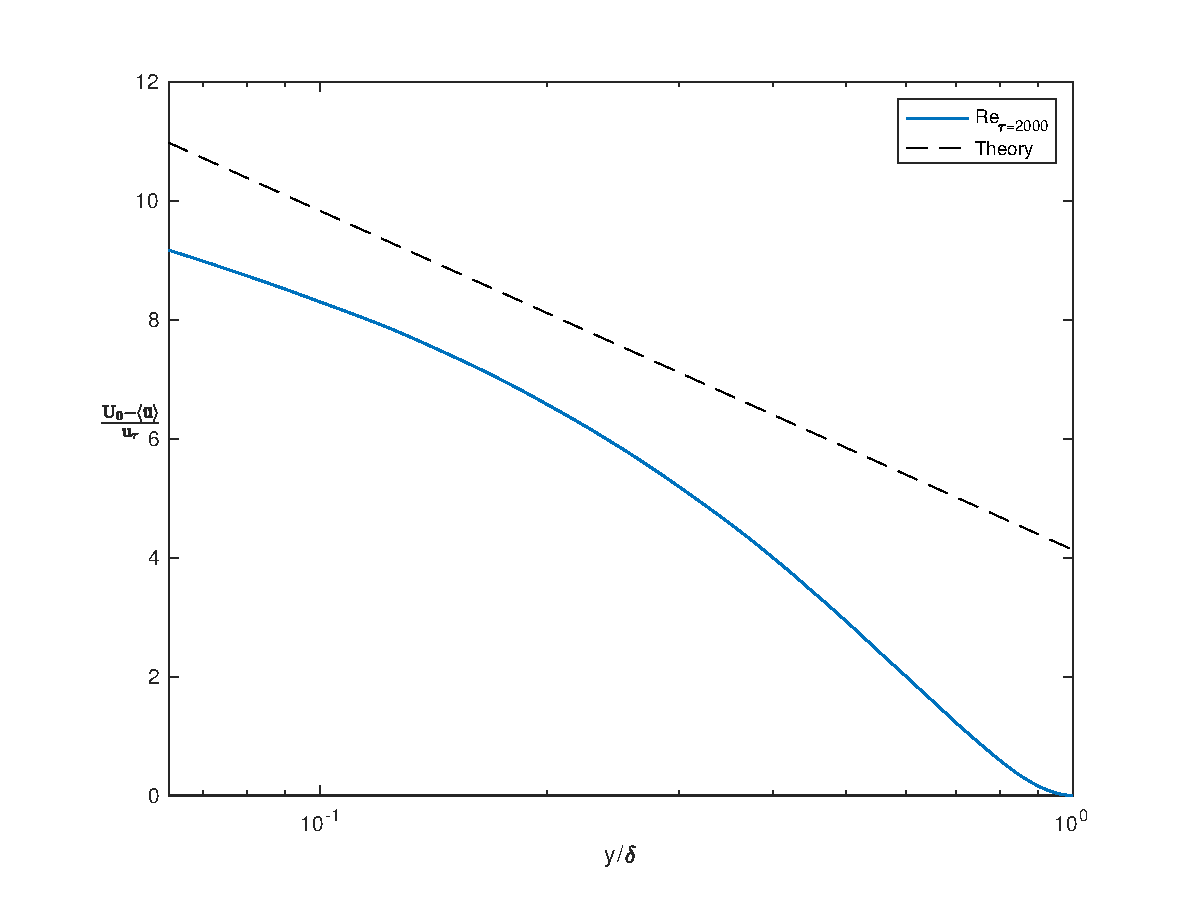
\includegraphics[scale=0.55]{grafici/velocity_defect_2000.eps}
\caption{Velocity defect for a $Re_{\tau}=2000$ simulation}
\label{velocity:defect:2000}
\end{center} 
\end{figure}

The errors present in the mean flow tend to amplify their magnitude when dealing with the fluctuating terms.\par
Despite of this the region of main interest, which is limited to few wall-units, seems to be not influenced by such the errors.  \par
By looking at the \emph{rms} profiles sketched in figure~\ref{budget:2000}, we can clearly see that the wall-normal fluctuating term remains approximately zeros until we reach $t\approx10$. This means that despite the higher $Re_{\tau}$, the turbulence still exhibit itself as a bi-dimensional phenomena close to the wall, exactly what happened also for the lower Reynolds simulations.\par

\begin{figure}
\begin{center}
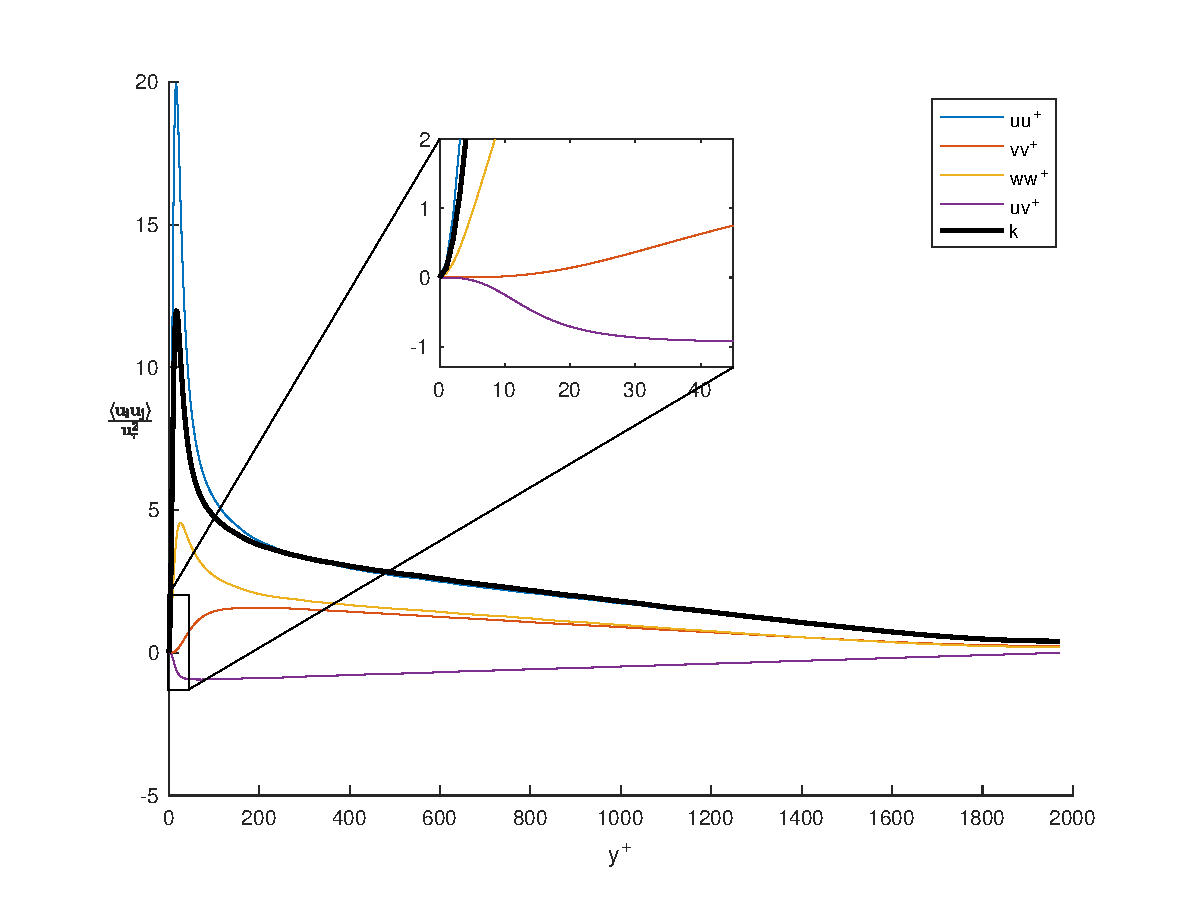
\includegraphics[scale=0.55]{grafici/budget+k_2000.eps}
\caption{\emph{rms} terms for a $Re_{\tau}=2000$ simulation}
\label{budget:2000}
\end{center} 
\end{figure}


Although the values presented in this figure are quantitatively wrong, figure~\ref{rms:2000} present the qualitative behavior of the \emph{rms} in a $Re_{\tau}=2000$ simulation. The raise in Reynolds number modify the fluctuations distribution with a generalized upward shift. Despite this increase the peaks coordinate tend to remain approximately constant. The knee tends to move rightward for all the \emph{rms} terms, towards the centerline. Also the outer-cycle peaks tend to exhibit an upward shift.\\~\par

\begin{figure}
\begin{center}
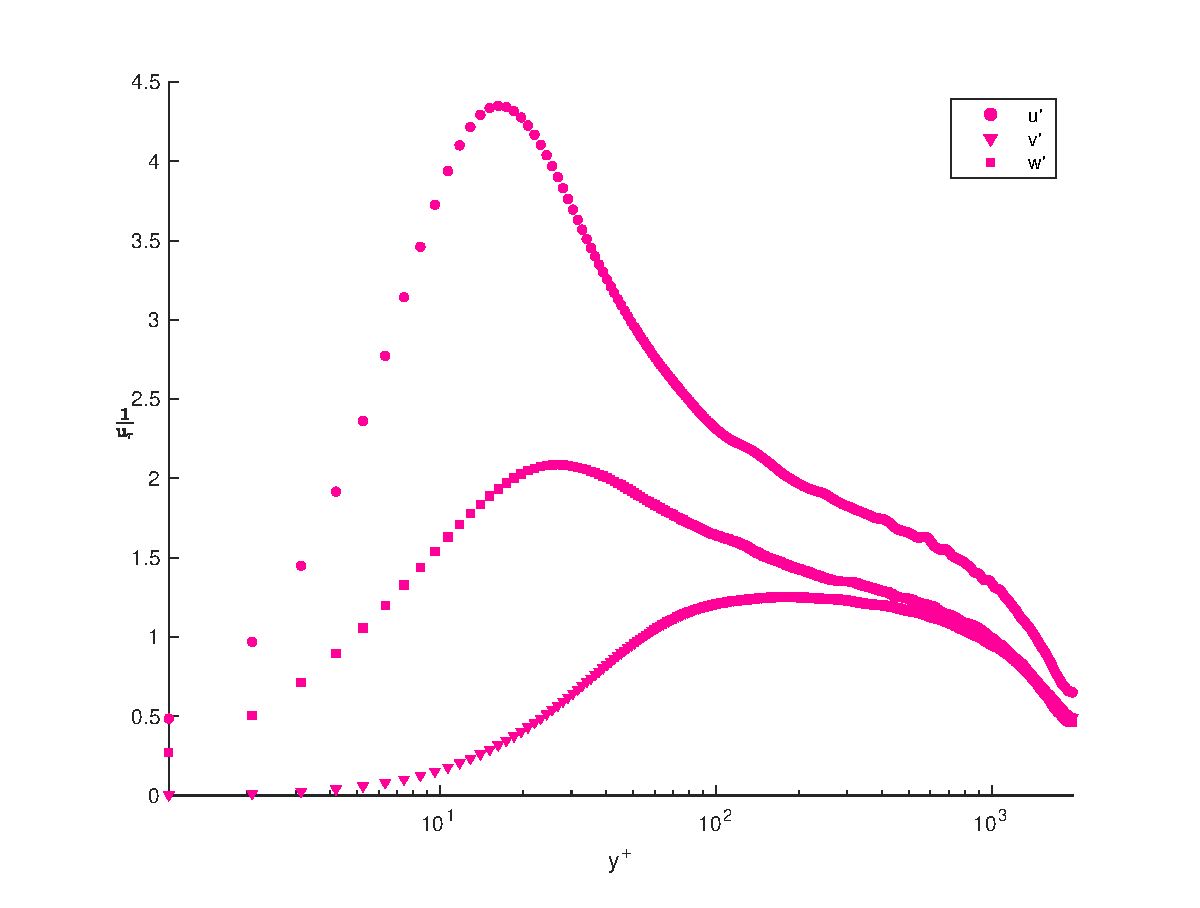
\includegraphics[scale=0.55]{grafici/rms_2000.eps}
\caption{\emph{rms} behavior on a $Re_{\tau}=2000$ simulation}
\label{rms:2000}
\end{center} 
\end{figure}

\begin{figure}
\begin{center}
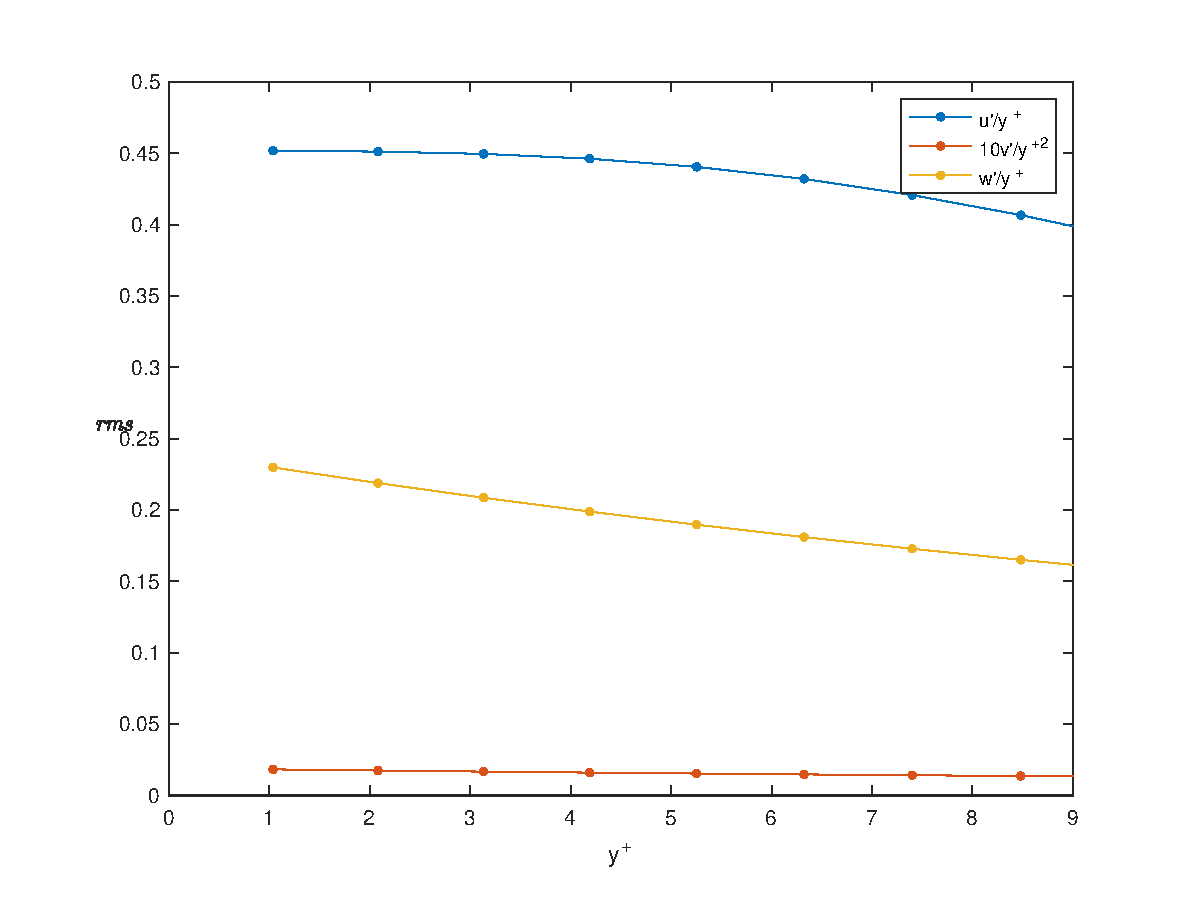
\includegraphics[scale=0.55]{grafici/wall_rms_2000.eps}
\caption{Normalized \emph{rms} close to the wall for a $Re_{\tau}=2000$ simulation}
\label{wall:rms:2000}
\end{center} 
\end{figure}

The streamwise and spanwise \emph{rms} terms tends to be higher since they leave the wall, this can be caught by comparing figure~\ref{wall:rms:2000} with figure~\ref{wall:rms:1000}. As can be recovered from the plot, such curves exhibit a linear growth for a wider range of wall coordinates, with respect to previous simulations. \par
The wall-normal fluctuation develops perfectly as $y^{+2}$ and its starting value is lower than the ones in previous simulations.\\~\par


For what concern about the \emph{production} term of the turbulent kinetic energy, according to figure~\ref{tke:prod:2000}, we can see that there are no changes to the profile, with the peak which remains near $y\approx12$. \\~\par

The normalized total shear stress profile is presented in figure~\ref{stresses:2000}. The graph exhibit the typical profile, with the Reynolds stresses that grows immediately and reach their peak before $y^{+}\approx 100$. \par
The crossing point between the viscous stress and Reynolds ones is still around $y\approx12$. This will be shown in the next chapter with an higher level of detail.


\begin{figure}
\begin{center}
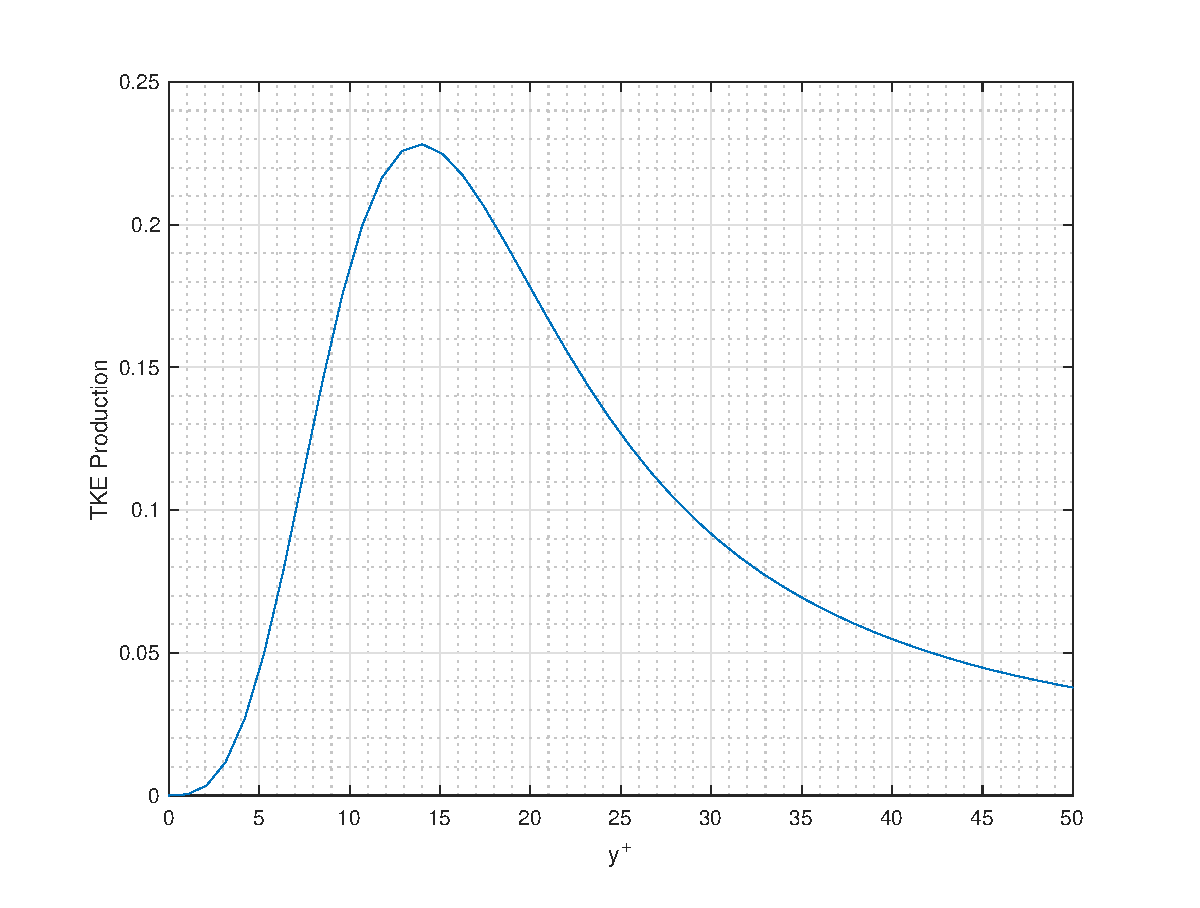
\includegraphics[scale=0.55]{grafici/tke_prod_2000.eps}
\caption{Production term of the TKE eq. for a $Re_{\tau}=2000$ simulation}
\label{tke:prod:2000}
\end{center} 
\end{figure}

\begin{figure}
\begin{center}
\includegraphics[scale=0.55]{grafici/stresses_2000.eps}
\caption{Normalized total shear stress for a $Re_{\tau}=2000$ simulation}
\label{stresses:2000}
\end{center} 
\end{figure}
\section{Reynolds effects}
We are now interested to catch the effects of the Reynolds on our statistics.\\~\par
The firstly macroscopical effect that we face is a shift, towards higher values, of the mean velocity profile. The shadowed area of figure~\ref{mean:comparison} let us enjoy the previous statement. According to this graph we can see a progressive narrowing of the region subjected to the higher shear stress, as the Reynolds number becomes larger.\par
Under the previous graph we reported the same quantity, but presented in semi-logaritmic scale, using both inner and outer scaling.
The first plot of figure~\ref{loglaw:comparison} highlights the results of the simulations and the theoretical behavior expectations.
In particular we can see that, despite the Reynolds number, all the simulations present the linear $\bar{u}=y^{+}$ behavior expected in the viscous sublayer, and the logarithmic profile in the homonym region, with $k=0.41$ and $B=5.2$.\\~\par

\begin{figure}
\begin{center}
\includegraphics[scale=0.55]{grafici/u_mean_comparison.eps}
\caption{Mean velocity profile at $Re_{\tau}$ variation}
\label{mean:comparison}
\end{center}
\end{figure}
\begin{figure}
\begin{center}
\includegraphics[scale=0.55]{grafici/loglaw_comparison.eps}
\caption{The law of the wall, in inner and outer scaling, at $Re_{\tau}$ variation}
\label{loglaw:comparison}
\end{center}
\end{figure}


Differently, the Reynolds stresses and the viscous stress exhibit dependance on the Reynolds number.\par
Figure~\ref{shear:comparison} shows how the shear stress components modify as the Reynolds number increase. \par
Focusing on the normalized Reynolds stresses graph we can clearly see that, as the $Re_{\tau}$ increase, the region subjected to this kind of stresses becomes larger, with the peak moving towards the wall. Such kind of stress is associated with the fluid turbulent motions, therefore it was expectable a raise of this components as we move towards a more turbulent flow. \par

\begin{figure}
\begin{center}
\includegraphics[scale=0.55]{grafici/shear_comparison.eps}
\caption{Normalized shear profiles at $Re_{\tau}$ variation}
\label{shear:comparison}
\end{center}
\end{figure}

\begin{figure}
\begin{center}
\includegraphics[scale=0.55]{grafici/y12.eps}
\caption{Particular of the shear stress, at $Re_{\tau}$ variation}
\label{y12}
\end{center}
\end{figure}

On the other side the contribute of the viscous stress, associate to $\partial{\bar{u}}/\partial{t}$, is maximum at the wall and tends to become negligible as we move towards the centerline. \par
As testified by figure~\ref{loglaw:comparison}, the higher is the Reynolds and the wider is the area subjected to logarithmic profile, hence smaller is the area subjected to strong variation of the mean velocity profile with the wall-normal coordinate. This fact reflects on our shear component reducing its range of effectiveness to few units, close to the wall, as the $Re$ grows.\par
Although, in terms of outer scaling, the stress components are subjected to strong variations, in inner scaling we can see, in figure~\ref{y12}, that the point at which the two components cross themself remains quite constant, with an $y^{+}$ around 12 wall-units.\\~\par


\begin{figure}
\begin{center}
\includegraphics[scale=0.55]{grafici/cf.eps}
\caption{Dependance of the $c_{f}$ from $Re_{b}$}
\label{cf}
\end{center}
\end{figure}


One of the most important flow property for wall bounded flows is the friction coefficient.
The $c_{f}$ has been studied in detail by many famous authors of the past: Nikuradse, Prandtl, Blasius just to cite some of them. \par
In our simulations we computed the skin friction coefficient based on the definition provided by~\cite[279]{pope}, based on centerline velocity $(U_{0})$ and the $Re_{b}$ of the channel.
The quantities have been defined as
\begin{equation*}
c_{f}= 2(\frac{u_{\tau}}{U_{0}})^{2}	\quad~\quad~\quad~\quad	Re_{b}= \frac{2 U_{b} \delta}{\nu},
\end{equation*}
and the results have been reported on figure~\ref{cf}. \par
Our $c_{f}$ shows good fitting with the results of the experimental campaign of Dean reported in~\cite{Dean}.





\chapter{Conclusions \& Further Works}
I am glad to say that we have reached our original goal to provide a scalable DNS solver through the usage of the MPI technology. \par
The code revealed to be robust, being capable of working both with small datasets then extra large ones, without suffering lacks or losses of performances.
Furthermore the possibility to perform live post-processing of the data, instead of writing them, allows to save terabytes of memory, allowing the code to run also on networks of commodity hardware. \\~\par
During our simulations we experienced a linear gain in performances, as highlighted by figure~\ref{speedup:trend}, while working with larger, and more interesting, sets of data. \par
The fundamental restriction imposed by the original code about the number of parallel tasks has been removed, bringing the theoretical number of parallel processes to be limited by the product of $nx \times nz$ modes. \\~\par
The engine developed is flexible and since is not affected by the geometry of the problem could be adapted quickly to carry out boundary layers simulations, just by imposing different boundary conditions, or can be used to solve pipe flows simulations.\\~\par
Although we are satisfied by this solver, we would like to highlight that by changing few rows, a possible forward step in terms of efficiency can be made.
In fact, by adopting the OpenMP technology we could employ more efficient functions to perform intra-nodal informations exchange. With today tendency of the HPC processors to increase the number of threads, instead of the number of physical CPU, this evolution, towards the so called \emph{hybrid-programming} seems mandatory.


\backmatter
\addcontentsline{toc}{chapter}{\bibname} 
\printbibliography

\end{document}
